%%%%%%%%%%%%%%%%%%%%%%%%%%%%%%%%%%%%%%%%%%%%%%%%%%%%%%%%%%%%%%%%%%%%%%%%%%%%%%%%
% University of Western Ontario Thesis Template
% By: Justin Quinn Veenstra, 2010
% With thanks to Mr. (soon to be Dr.) Will Robertson.


\documentclass[12pt,twoside]{report}
%% Decomment next line to use PostScript fonts
%%\UsePackage{times}
%%%%%%%%%%%%%%%%%%%%%%%%%%%%%%%%%%%%%%%%%%%%%%%%%%%%%%%%%%%%%%%%%%%%%%%%
%%                                                                    %%
%%                    ***   I M P O R T A N T   ***                   %%
%%                                                                    %%
%% Fill in the following fields with the required information:        %%
%%  - \department{...}  name of the graduate department               %%
%%  - \degree{...}      name of the degree obtained                   %%
%%  - \author{...}      name of the author                            %%
%%  - \title{...}       title of the thesis                           %%
%%  - \gyear{...}       year of graduation                            %%
%%  - \super{...}    supervisor
%%  - \firstname, \middlename, \lastname... there is additional documentation by the actual fields, so I'll leave it at that
%%%%%%%%%%%%%%%%%%%%%%%%%%%%%%%%%%%%%%%%%%%%%%%%%%%%%%%%%%%%%%%%%%%%%%%%
\usepackage[titletoc,title]{appendix}
\usepackage{graphicx,amsmath,amsfonts,amssymb,bbm,amsthm}
\usepackage[byname]{smartref}
%\usepackage{hyperref} %comment out for hardcopy
\usepackage{txfonts}
\usepackage{tocloft}
\usepackage{natbib}
\usepackage{chapterbib}
\usepackage{subcaption}
\usepackage{tikz}
\usepackage{array}
\usepackage{float}
\usepackage{pifont}
\usepackage{hyperref}
\usepackage{blindtext}
\usepackage{pdfpages}
\usepackage{multirow}
\usepackage{color}
\usepackage[framed,numbered,autolinebreaks,useliterate]{mcode}
\usepackage{xcolor}
% \newcommand{\xin}[1]{{\color{cyan} #1}}
% \newcommand{\geo}[1]{{\color{magenta}#1}}
% \newcommand{\ak}[1]{{\color{red}#1}}
%--------------------------------------
\usepackage[utf8]{inputenc}
\usepackage[T1]{fontenc}
%--------------------------------------
 
%German-specific commands
%--------------------------------------
%\usepackage[ngerman]{babel}
%--------------------------------------
\hypersetup{
    colorlinks=false,
    filecolor=black,      
    urlcolor=black,
}
\renewcommand{\baselinestretch}{2}
\makeatletter
\numberwithin{figure}{chapter}
\newenvironment{acknowledgements}%
{\clearemptydoublepage
 \begin{center}
  \section*{Acknowledgements}
 \end{center}
 \begingroup
}{\newpage\endgroup}

\newenvironment{dedication}%
{\clearemptydoublepage 
 \begin{center}
  \section*{Dedication}
 \end{center}
 \begingroup
}{\newpage\endgroup}

\newenvironment{preliminary}%
{\pagestyle{plain}\pagenumbering{roman}}%
{\pagenumbering{arabic}}

\addtoreflist{chapter}
\newtheorem{theorem}{Theorem}[section]
\newtheorem{lemma}[theorem]{Lemma}
\newtheorem{proposition}[theorem]{Proposition}
\newtheorem{corollary}[theorem]{Corollary}

%\newenvironment{proof}[1][Proof]{\begin{trivlist}
%\item[\hskip \labelsep {\bfseries #1}]}{\end{trivlist}}
\newenvironment{definition}[1][Definition]{\begin{trivlist}
\item[\hskip \labelsep {\bfseries #1}]}{\end{trivlist}}
\newenvironment{example}[1][Example]{\begin{trivlist}
\item[\hskip \labelsep {\bfseries #1}]}{\end{trivlist}}
\newenvironment{remark}[1][Remark]{\begin{trivlist}
\item[\hskip \labelsep {\bfseries #1}]}{\end{trivlist}}

%\newcommand{\qed}{\nobreak \ifvmode \relax \else
      %\ifdim\lastskip<1.5em \hskip-\lastskip
      %\hskip1.5em plus0em minus0.5em \fi \nobreak
      %\vrule height0.75em width0.5em depth0.25em\fi}

% Default values for title page.

%% To produce output with the desired line spacing, the argument of
%% \spacing should be multiplied by 5/6 = 0.8333, so that 1 1/2 spaced
%% corresponds to \spacing{1.5} and double spaced is \spacing{1.66}.
\def\normalspacing{1.25} % default line spacing


%% Define the "thesis" page style.
\if@twoside % If two-sided printing.
\def\ps@thesis{\let\@mkboth\markboth
   \def\@oddfoot{}
   \let\@evenfoot\@oddfoot
   \def\@oddhead{
      {\sc\rightmark} \hfil \rm\thepage
      }
   \def\@evenhead{
      \rm\thepage \hfil {\sc\leftmark}
      }
   \def\chaptermark##1{\markboth{\ifnum \c@secnumdepth >\m@ne
      Chapter\ \thechapter. \ \fi ##1}{}}
   \def\sectionmark##1{\markright{\ifnum \c@secnumdepth >\z@
      \thesection. \ \fi ##1}}}
\else % If one-sided printing.
\def\ps@thesis{\let\@mkboth\markboth
   \def\@oddfoot{}
   \def\@oddhead{
      {\sc\rightmark} \hfil \rm\thepage
      }
   \def\chaptermark##1{\markright{\ifnum \c@secnumdepth >\m@ne
      Chapter\ \thechapter. \ \fi ##1}}}
\fi

\pagestyle{thesis}
% Set up page layout.
\setlength{\textheight}{9in} % Height of the main body of the text
\setlength{\topmargin}{-.5in} % .5" margin on top of page
\setlength{\headsep}{.5in}  % space between header and top of body
\addtolength{\headsep}{-\headheight} % See The LaTeX Companion, p 85
\setlength{\footskip}{.5in}  % space between footer and bottom of body
\setlength{\textwidth}{6.25in} % width of the body of the text
\setlength{\oddsidemargin}{.25in} % 1.25" margin on the left for odd pages
\setlength{\evensidemargin}{0in} % 1.25"  margin on the right for even pages

% Marginal notes
\setlength{\marginparwidth}{.75in} % width of marginal notes
\setlength{\marginparsep}{.125in} % space between marginal notes and text

% Make each page fill up the entire page. comment this out if you
% prefer. 
\flushbottom

\setcounter{tocdepth}{3} % Number the subsubsections 
\def\normalspacing{1.25} % default line spacing

\newcommand\isco[1]{%
  \edef\@tempa{#1}%
  \def\@tempb{}%
  \ifx\@tempa\@tempb
	\else \\\underline{Co-Supervisor:}\vspace{0.35in}\\\dots\dots\dots\dots\dots\dots\dots\\{#1}\\
  \fi
}

\newcommand\isjoint[1]{%
  \edef\@tempa{#1}%
  \def\@tempb{}%
  \ifx\@tempa\@tempb
	\else \\\underline{Joint Supervisor:}\vspace{0.35in}\\\dots\dots\dots\dots\dots\dots\dots\\{#1}\\
  \fi
}

\newcommand\isalt[1]{%
  \edef\@tempa{#1}%
  \def\@tempb{}%
  \ifx\@tempa\@tempb
	\else \\\underline{Alternate Supervisor:}\vspace{0.35in}\\\dots\dots\dots\dots\dots\dots\dots\\{#1}\\
  \fi
}

\newcommand\isdefinedsig[1]{%
  \edef\@tempa{#1}%
  \def\@tempb{}%
  \ifx\@tempa\@tempb
	\else \\ \dots\dots\dots\dots\dots\dots\dots\\{#1}\\
  \fi
}
\newcommand\isdefinedspinetitle[1]{%
  \edef\@tempa{#1}%
  \def\@tempb{}%
  \ifx\@tempa\@tempb
	\else (Spine title: #1)\\
  \fi
}
\newcommand\coauthor[1]{%
  \edef\@tempa{#1}%
  \def\@tempb{}%
  \ifx\@tempa\@tempb
	\else \newpage \Large Co-Authorship Statement\normalsize\\\indent\\#1\\
  \fi
}

\newcommand\acknowlege[1]{%
  \edef\@tempa{#1}%
  \def\@tempb{}%
  \ifx\@tempa\@tempb
	\else \newpage \Large Acknowlegements\normalsize\\\indent\\#1\newpage
  \fi
}

%\renewcommand{\appendixtocname}{\Huge \textbf{List of Appendices} \normalsize}
\newcommand{\blank}{\hspace{-2mm}}
\newcommand{\super}{Dr. Lindi M. Wahl} %supervisor
%\newcommand{\superj}{Dr. A. Manning} %joint supervisor, if there is one, leave blank if not (lbin)... only one of the three.
\newcommand{\superc}{} %co-supervisor, if there is one, leave blank if not (lbin)
\newcommand{\supera}{} %alternate supervisor, if there is one, leave blank if not (lbin)
\newcommand{\sco}{Dr. W. J. Braun}  %member of supervisory committee
\newcommand{\sct}{Dr. A. Bing}  %other member of supervisory committee (lbin)
\newcommand{\examo}{Dr. Q. Ring}  %examining committee (up to four, if less leave blank)
\newcommand{\examt}{Dr. W. Fing}
\newcommand{\examth}{Dr. G. Hing}
\newcommand{\examf}{}
\newcommand{\department}{Applied Mathematics}
\newcommand{\degree}{Doctor of Philosophy}
\newcommand{\firstname}{Amjad}
\newcommand{\middlename}{}
\newcommand{\lastname}{Khan}
%\renewcommand{\author}[1]{\ifx\empty#1\else\gdef\@author{#1}\fi} 
\newcommand{\authorname}{{\firstname} {\middlename} {\lastname}}
\newcommand{\titl}{Phage-bacteria interaction and the evolution of prophage sequences}
\newcommand{\spinetitle}{}%only if the above is more than 60 characters
\newcommand{\thesisformat}{Integrated Article} %or Integrated Article
\newcommand{\gyear}{\number\year}
\newcommand{\makecoauthor}{
I, Amjad Khan, declare that this thesis titled, “Phage-bacteria interaction and prophage sequences in bacterial genomes” has been written by me under the supervision of  Dr.  Lindi M. Wahl. 

\textbf{Chapter 2}: Phage therapy and antibiotics for biofilm eradication: a predictive model, has been published as a book chapter co-authored with L.M. Wahl and P. Yu in Recent Advances in Mathematical and Statistical Methods. AK developed the model with supervisory input from LMW, and AK performed the analysis. PY confirmed the analysis. AK drafted the paper. AK, PY and LMW finalized the paper.

\textbf{Chapter 3}: Quantifying the forces that maintain prophages in bacterial genomes, has been accepted as journal article co-authored with L.M. Wahl in Journal of Theoretical Population Biology. AK and LMW developed the model. AK and LMW contributed equally to the bioinformatics analysis. AK wrote the code, executed and analyzed all optimization results. AK drafted all results. AK and LMW jointly wrote the paper.

\textbf{Chapter 4}: The genetic repertoire of prophages, has been submitted for publication co-authored with L.M. Wahl and A.R. Burmeister in PLOS Computational Biology. AK, ARB and LMW designed the study. AK and LMW developed the mathematical and computational approaches. AK, ARB and LMW analysed the data. AK, ARB and LMW wrote the manuscript.
}
\newcommand{\makeacknowlege} {
I am thankful to my supervisor Lindi Wahl for continued support and insights. My supervisor's guidance helped me in all the time of research and writing of this thesis. I could not have imagined having a better supervisor and mentor for my Ph.D study. I am also indebted to Professor Pei Yu (Department of Applied Mathematics, UWO) and  Alita Burmeister (Associate Research Scientist in Ecology and Evolutionary Biology, Yale University) for several insightful comments.  Lastly, I would like to thank the professors and staff in the Department of Applied Mathematics, Western University, for their help during my graduate studies.
}
\newcommand{\listappendixname}{List of Appendices}
\newlistof{myappendices}{app}{\listappendixname}
\newcommand{\myappendices}[1]{%
\addcontentsline{app}{myappendices}{#1}\par}

\renewcommand{\maketitle}
{\begin{titlepage}
   \setcounter{page}{1}
   %% Set the line spacing to 1 for the title page.
   %\begin{spacing}{1} 
   \begin{large}
   \begin{center}
      \mbox{}
      \vfill
      {\MakeUppercase{\titl}}\\
      \isdefinedspinetitle{\spinetitle}
      (Thesis format: \thesisformat)\\
      \vfill
      by \\
      \vfill
      {\firstname} \underline{\lastname}\\
      \vfill
      Graduate Program in {\department}\\
      \vfill
		A thesis submitted in partial fulfillment\\
		of the requirements for the degree of\\
		\degree\\
		\vfill
		The School of Graduate and Postdoctoral Studies\\
		The University of Western Ontario\\
		London, Ontario, Canada\\
		\vfill
      {\copyright} {\authorname} {\gyear}  \\
      \vspace*{.2in}
   \end{center}
   \end{large}
%   \end{spacing}
   \end{titlepage}

}%\maketitle

\newcommand{\makecert}{
   \setcounter{page}{2}
\vfill
\begin{center}
\large
THE UNIVERSITY OF WESTERN ONTARIO\\
School of Graduate and Postdoctoral Studies\\
\vfill
\textbf{CERTIFICATE OF EXAMINATION}
\end{center}

\vfill
\begin{table}[ht]
\begin{minipage}[t]{0.5\linewidth} %tabular instead?
\begin{tabular}{l}
\underline{Supervisor:}\vspace{0.35in}
\isdefinedsig{\super}
\isco{\superc}
\isjoint{\superj}
\isalt{\supera}
\\
\underline{Supervisory Committee:}\vspace{0.35in}
\isdefinedsig{\sco}\vspace{0.15in}
\isdefinedsig{\sct}
\end{tabular}
\vfill
\end{minipage}
\hspace{0.5in}
\begin{minipage}[t]{0.5\linewidth}
\begin{tabular}{l}
\underline{Examiners:} \\\vspace{.5cm}
\isdefinedsig{\examo}\\
\isdefinedsig{\examt}\\
\isdefinedsig{\examth}\\
\isdefinedsig{\examf}
\end{tabular}
\vfill
\end{minipage}
\vfill
\end{table}
\vfill
\begin{center}
The thesis by \\ \vfill
\textbf{\firstname{} \middlename{} \underline{\lastname}}\\
\vfill
entitled:\\\vfill
\textbf{\titl}\\\vfill
is accepted in partial fulfillment of the \\
requirements for the degree of\\
\degree\\
\end{center}
\begin{table}[ht]
\begin{minipage}[t]{0.5\linewidth}
\begin{tabular}{l}
\dots\dots\dots\dots\dots\\
Date
\end{tabular}
\end{minipage}
\hspace{0.5in}
\begin{minipage}[t]{0.5\linewidth}
\begin{tabular}{l}
\dots\dots\dots\dots\dots\dots\dots\dots\dots\dots\\
Chair of the Thesis Examination Board
\end{tabular}
\end{minipage}
\end{table}

}

\makeatother
\begin{document}

%% ***   NOTE   ***
%% You should put all of your '\newcommand', '\newenvironment', and
%% '\newtheorem's (in other words, all the global definitions that you
%% will need throughout your thesis) in a separate file and use
%% "\input{filename}" to input it here.


%% This sets the page style and numbering for preliminary sections.
\begin{preliminary}

%% This generates the title page from the information given above.
%\maketitle
%\addcontentsline{toc}{chapter}{Certificate of Examination}
%\makecert
%\newpage
% \addcontentsline{toc}{chapter}{Co-Authorship Statement}
% \coauthor{\makecoauthor}  %comment this out if none
% \newpage
% \addcontentsline{toc}{chapter}{Acknowledgements}
% \acknowlege{\makeacknowlege}	%as above
\addcontentsline{toc}{chapter}{Abstract}
\Large\begin{center}\textbf{Abstract}\end{center}\normalsize
%%  ***  Put your Abstract here.   ***
%% (150 words for M.Sc. and 350 words for Ph.D.)

In this investigation, we examined the interaction of phages and bacteria in bacterial biofilm colonies,  the evolution of prophages (viral genetic material inserted into the bacterial genome) and their genetic repertoire. To study the synergistic effects of lytic phages and antibiotics on bacterial biofilm colonies, we have developed a mathematical model of ordinary differential equations (ODEs).  We have also presented a mathematical model consisting of a partial differential equation (PDEs), to study evolutionary forces acting on prophages.  We fitted the PDE model to three publicly available databases and were able to show that induction is the prominent fate of intact prophages, with an average prophage loss of only 1\% of its genome before induction.  We also demonstrate that there is a tipping point at which the relation between prophage and bacteria transforms from being parasitic to mutualistic. Lastly, we investigated annotated prophages from two well-studied prophage databases. These genes were accessed using PHASTER, a bioinformatics tool to identify prophages in bacterial genomes. From this analysis, we observed that genes involved in phage lytic function are preferentially lost, while integrase and transposase are preferentially enriched in smaller prophages.  We have also developed an ODE model and have carried out gene-level simulations to get more insight into the genetic repertoire of prophages.
The results of our ODE model and gene-level simulations are in agreement with prophage repertoire data.   

\vfill
\textbf{Keywords:} Bacteriophage, Bacteria, Biofilm, Phage therapy, Mathematical model, Prophage \& domestication, Genome evolution, Individual-based model, Genetic repertoire, Defective prophages.
\newpage
\addcontentsline{toc}{chapter}{Summary for lay audience}
\Large\begin{center}\textbf{Summary for lay audience}\end{center}\normalsize
%%  ***  Put your Abstract here.   ***
%% (150 words for M.Sc. and 350 words for Ph.D.)

{Bacteriophages are viral predators of bacteria. Upon infecting bacteria, bacteriophages either kill the host bacteria or enter a long-term genetic association with the bacterial host. The ability of bacteriophages to kill bacterial cells is used as a therapeutic strategy to cure bacterial infections, called phage therapy.  If the bacteriophage enters a long-term association with the host, the viral genome integrated into the host bacterial genome is called a prophage. In this investigation, using mathematical modeling approaches, we study the synergistic effects of phage therapy and antibiotics on bacterial biofilm colonies, the evolution of prophages and the genetic composition of prophages.}    

\newpage
\addcontentsline{toc}{chapter}{Co-Authorship Statement}
\Large\begin{center}\textbf{Co-Authorship Statement}\end{center}\normalsize
\makecoauthor
\newpage
\addcontentsline{toc}{chapter}{Acknowledgements}
\Large\begin{center}\textbf{Acknowledgements}\end{center}\normalsize
\makeacknowlege
\newpage
\tableofcontents\newpage
\newpage
\addcontentsline{toc}{chapter}{List of Figures}
\listoffigures
\newpage
\addcontentsline{toc}{chapter}{List of Tables}
\listoftables\newpage
\addcontentsline{toc}{chapter}{List of Appendices}
\listofmyappendices\newpage
%\addcontentsline{toc}{chapter}{List of Abbreviations, Symbols, and Nomenclature}
%\large List of Abbreviations, Symbols, and Nomenclature \normalsize
%\newpage
\end{preliminary}
%% End of the preliminary sections: reset page style and numbering.

%%%%%%%%%%%%%%%%%%%%%%%%%%%%%%%%%%%%%%%%%%%%%%%%%%%%%%%%%%%%%%%%%%%%%%%%
%%                                                                    %%
%%                    ***   I M P O R T A N T   ***                   %%
%%                                                                    %%
%% Put your Chapters here; the easiest way to do this is to keep each %%
%% chapter in a separate file and \include all the files right here.  %%
%% Note that each chapter file should start with the line             %%
%% "\chapter{ChapterName}".  Note that using "\include" instead of    %%
%% "\input" makes each chapter start on a new page.                   %%
%%%%%%%%%%%%%%%%%%%%%%%%%%%%%%%%%%%%%%%%%%%%%%%%%%%%%%%%%%%%%%%%%%%%%%%%

\chapter{Introduction}
\section{Introduction}

 Bacteria were one of the first life forms to appear on earth and have a profound and diverse impact on our lives \citep{abedon_bacteriophage_2008}.  It has been shown that the ratio of human cells to bacterial cells, in the human body, is close to 1:1 \citep{sender_revised_2016}, an update of the popular estimate that bacterial cells outnumber human cells in our body by the ratio 10:1 \citep{luckey_introduction_1970,savage_microbial_1977}. In 1915, the British microbiologist Fredrick Twort \citep{twort_investigation_1915} observed the phenomenon of clearing in a solution of bacteria and thought that it was caused by an enzyme responsible for killing bacteria \citep{weitz_quantitative_2017}. In 1917, the French physician Felix d’Herelle observed the same clearing phenomenon and speculated that an organism, which he called bacteriophage (phage for short) or “bacteria eater”, was responsible for killing the bacteria \citep{dHerelle_1917}. After the direct visualization of these bacteria eaters under the electron microscope, it was established that these bacteria eaters are organisms \citep {borries_bakterien_1938}, the bacteriophages.  Phages outnumber their bacterial hosts by a ratio of approximately 10:1 \citep{bergh_high_1989}, making them  the most abundant microorganisms in the biosphere \citep{rohwer_global_2003, clokie_phages_2011} and have been critical players in the evolutionary history of bacteria \citep{stern_phage-host_2011}. 

\section{Bacteriophages}
\subsection{Phage life cycle}
Although some viruses do not exclusively depend on their host for replication and carry with them genes needed for the processes thought to be the distinguishing characteristic of life \citep{raoult_1.2-megabase_2004}, most viruses require a host for their replication. A phage starts its life cycle by  attaching to a specific receptor on the surface of the bacterial host. Once attached, the phage injects its viral genome into the host cell. After injection, these viral genomes can take several possible pathways, of which the most well-known are:
(1) the viral genome takes over the host's cellular machinery, the viral genome is replicated and the structural components are produced, ultimately leading to the death of host cell and release of progeny virions into the environment, known as the lytic life cycle; and (2) the viral genome once inside the cell is integrated with the host bacterial genome, known as the lysogenic life cycle. 

 Phages that can follow only the lytic life cycle are called lytic phages whereas phages which follow either the lytic or lysogenic life cycle are called temperate phages. The majority of the identified temperate phages are double-stranded (ds) DNA viruses \citep{szekely_single-stranded_2016}, with the exception of a few single-stranded (ss) DNA temperate phages  \citep{krupovic_single-stranded_2015}. Integrated viral DNA of a temperate phage is referred to as a prophage and the bacterial cell carrying prophage or prophages is called a lysogen \citep{lwoff_lysogeny_1953}.  These prophage sequences are transmitted vertically with the genome of the bacterial host as the host cell divides into daughter cells \cite{feiner_new_2015}. 

 
 Since the discovery of phages, the ability of lytic phages to eradicate a bacterial population has been used to treat bacterial infectious diseases in humans, animals, and plants \citep{abedon_editorial:_2017,myelnikov_alternative_2018}.  After the advent of antibiotics to treat infectious diseases, phage therapy was confined to particular regions of the world \citep{myelnikov_alternative_2018}. Recently, due to the emergence of antibiotic-resistant bacteria, attention has been refocused on phage as a weapon against bacterial infectious diseases \citep{abedon_editorial:_2017, bull_dynamics_2002}. 
 
 \subsection{Bacterial genome sequencing}
Bacterial genomes are compact as compared to eukaryotic genomes in a sense that bacterial genomes contain less noncoding DNA, see Figure~\ref{fig:compact}.
Bacterial genomes vary in size by at least an order of magnitude \citep {bobay_evolution_2017} and may be up to 30 Mb in size \citep{brown_genomes_2007}. Bacterial genomes are dynamic and are exposed to various events dominated by insertions and deletions of genetic elements \citep{sela_theory_2016}. To understand the role of bacteria in shaping our environment and to eliminate various bacterial diseases, a complete understanding of the bacterial genome is important. 

The year 1995 is marked as the year when the first two human pathogenic bacterial genomes, \textit{Haemophilus influenzae} \citep{fleischmann_whole-genome_1995} and \textit{Mycoplasma genetalium} \citep{fraser_minimal_1995}, were sequenced. Since then bacterial genome sequencing has undergone substantial development. From 1995 – 2009 only 2010 sequenced bacterial genomes were submitted to NCBI, this number has increased with the advent of modern technologies  and 213,581 bacterial genomes have been sequenced and submitted to NCBI (as of November 2019), see Figure~\ref{fig:seqgenomes}.  
  The process of extracting biological information from sequenced bacterial genome data and providing descriptive information to these features is called bacterial genome annotation.
   \begin{figure}[t]
    \centering
     \begin{subfigure}[t]{0.45\textwidth} 
    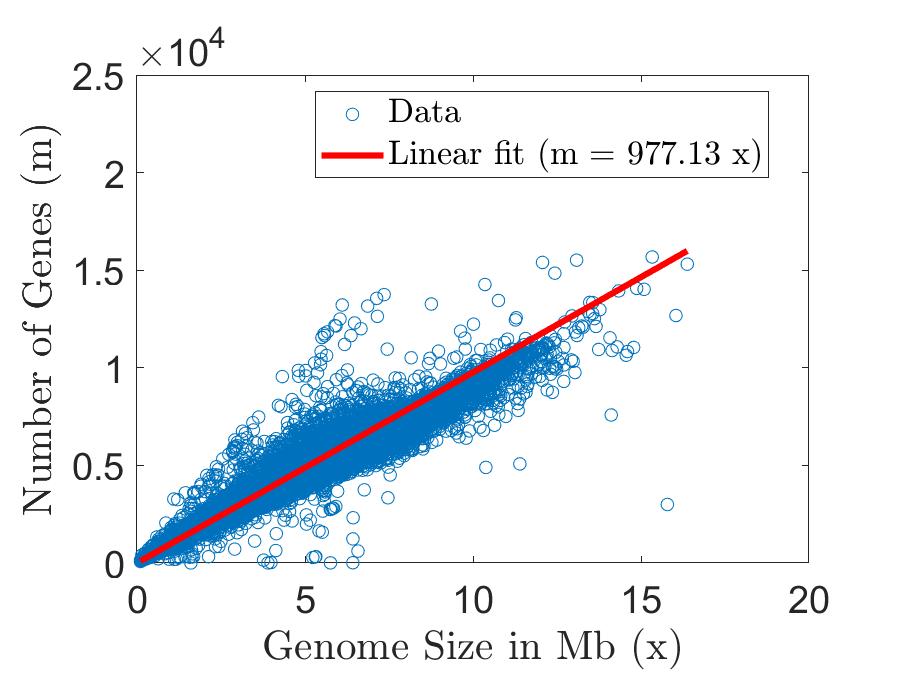
\includegraphics[scale=0.55]{bac}
     \subcaption{Number of genes versus bacterial genome size, showing a high correlation (correlation coefficient $r$ =0.984) between genome size and number of genes contained. }
     %\label{fig:brug_bar}
     \end{subfigure}\hfill
         \begin{subfigure}[t]{0.45\textwidth}
          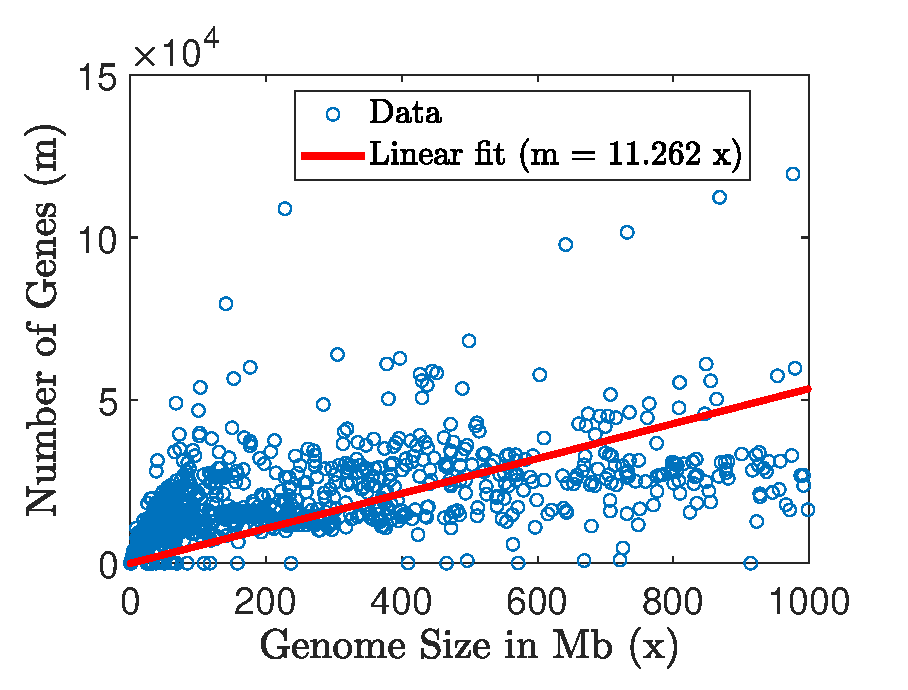
\includegraphics[scale=0.55]{eu}
            \subcaption[subfigcapskip = 50pt]{Number of genes versus eukaryotic genome size, showing a lower correlation ($r$ =0.624) between eukaryotic genome size and number of genes.}
            %\label{fig:}
    \end{subfigure}\hfill
    \caption[Prokaryotic genomes are compact as compared to eukaryotic genomes.]{Prokaryotic genomes are compact as compared to eukaryotic genomes. These data were downloaded from GenBank in November 2019 and consist of 190,618 bacterial genomes and 2,379 eukaryotic genomes.}
    \label{fig:compact}
\end{figure}
\begin{figure}[t]
    \centering
         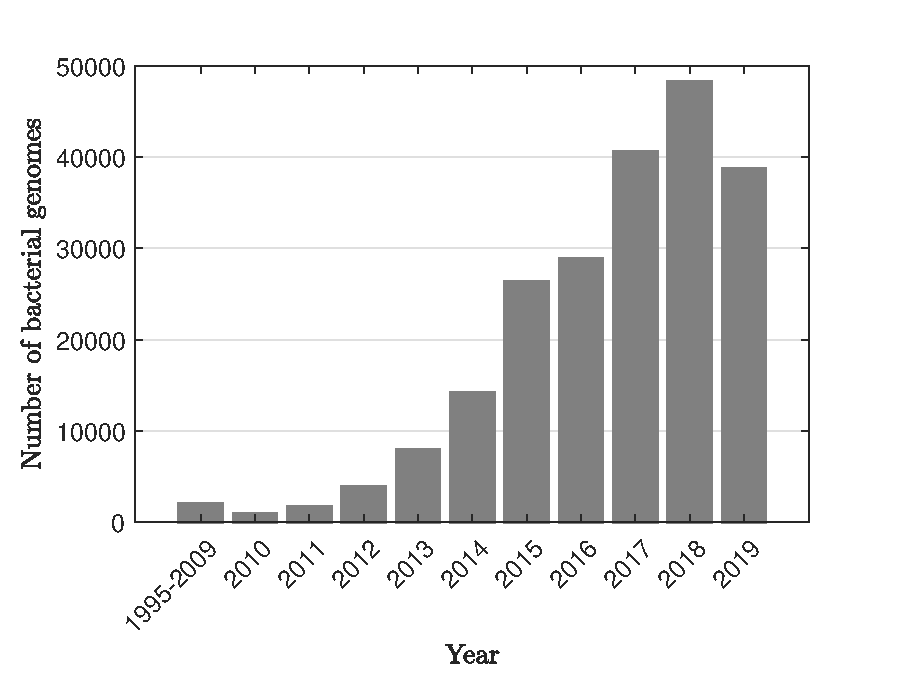
\includegraphics[scale=0.7]{bacseq}
         \caption[The number of bacterial genome sequences submitted to NCBI is growing rapidly.]{The number of bacterial genome sequences submitted to NCBI is growing rapidly. These data were downloaded from NCBI in November 2019.}
         \label{fig:seqgenomes}
\end{figure}
  \subsection{Prophage abundance and detection in bacterial genomes}
% [Be careful not to self-plagiarize.  None of the sentences in this section should be repeated in the introductory material of the later chapters.  Re-phrase here if they are the same sentences so that the papers can be inserted as chapters "as is".]
In the event of lysogeny, temperate phages can integrate their genome into different chromosomal sites of a bacterial genome. Phage $\lambda$ DNA integrates at a unique site in the bacterial genome \cite{tal_location_2014}, phage P2 integrates its genome at at least 10 different sites in the host bacterial genome \cite{barreiro_attachment_1992}, whereas phage Mu can integrate randomly into the host bacterial genome \cite{bukhari_random_1972}. Bacterial genome sequencing has revealed that prophages are not only frequently identified in pathogenic bacterial strains \citep{canchaya_impact_2004}, but are abundant in many bacterial genomes. Prophages may constitute up to 20\% of a bacterial genome \citep{casjens_prophages_2003}. The distribution of prophages in a bacterial genome is variable, ranging from no prophage to several prophages per bacterial genome  \citep{touchon_genetic_2016}. For example, the sequenced \textit{Escherichia coli} O157:H7 strain Sakai has been shown to contain 18 prophages which make up 16\% of its total genome content. 

Temperate phages, after integration with the bacterial genome, repress their lysis genes \citep{lawrence_where_2001} and are subject to mutations that are biased towards deletions \citep{casjens_prophages_2003}.  This mutational degradation may eliminate the ability of a prophage to enter into the lytic life cycle by deleting or damaging genes required for lysis and re-infection.  Prophages lacking the ability to enter into the lytic life cycle are called defective or cryptic prophages \cite{de_bruijn_prophages_1998}. It has been shown that defective prophages are abundant in bacterial genomes, for example, \textit{Escherichia coli} K-12 contains nine cryptic prophage elements in its genome \citep{wang_cryptic_2010}. 

A prophage, after insertion into the bacterial genome, becomes a part of the bacterial genome.  This relation between prophages and host bacterial cells is usually stable but intact prophage may initiate the lytic life cycle spontaneously \cite{ fothergill_effect_2011, james_differential_2012}, or in response to some environmental cues, or DNA damaging agents \cite{ barnhart_prophage_1976, lopez_induction_2014}, resulting in the killing of the host and release of progeny virions into the environment. This process is called the induction of a prophage and is very common in the bacterial world \cite{ alexeeva_spontaneously_2018}.  Some prophages, like $\lambda,$ excise from the bacterial chromosome to initiate the lytic life cycle, while others, like Mu, produce viral particles before excision from the host bacterial genome \citep{shapiro_molecular_1979}.

 Prophage sequences bring with them many genes, making prophage  a prominent source of genetic diversity within bacterial populations \cite{fortier_importance_2013}. Amongst the changes caused by prophages of particular interest has been the contribution of prophages to bacterial virulence and antibiotic resistance \cite{wagner_bacteriophage_2002,fortier_importance_2013, haaber_bacterial_2016}. 
 
Prophages can be identified in a bacterial genome using experimental or computational approaches. In the experimental approach, bacteria are usually exposed to UV light or other DNA-damaging conditions to cause the induction of prophages present in the bacterial genome. This technique clearly overlooks the presence of defective prophages as well as other prophages that could not induce.  Since a large number of sequenced bacterial genomes are publicly available, computational approaches to identify prophages are preferred.  

Since the early 2000s many computational approaches have been developed to find prophages in bacterial genomes. Different computational programs used to identify prophages include Dinucleotide abundance \citep{nicolas_mining_2002, srividhya_identification_2007}, Phage\_Finder \citep{fouts_phage_finder:_2006}, Prophage Finder \citep{bose_prophage_2006}, Prophinder \citep{lima-mendez_prophinder:_2008}, PHAST (PHAge Search Tool) \citep{zhou_phast:_2011}, PHASTER (PHAge Search Tool – Enhanced Release), an improved version of PHAST \citep{arndt_phaster:_2016},  PhiSpy \citep{akhter_phispy:_2012}, VirSorter \citep{roux_virsorter:_2015}, VRprofile \citep{li_vrprofile:_2017} and others. Using these computational tools it has been shown that prophages are abundant in bacterial genomes. PhiSpy \citep{akhter_phispy:_2012}, written in Python and C++, was used to identify 36,488 prophages from the analysis of over 11,000 bacterial genomes; 83\% of the bacterial genomes contained at least one prophage \citep{kang_prophage_2017}. In another study, PHAST \citep{zhou_phast:_2011} was used to identify 4122 prophages in 795 \textit{Acinetobacter baumannii} genomes, for an average of 5 prophages per bacterial genome \citep{costa_genomic_2018}. Of these prophages 78\% were identified as defective. Using PHASTER, Mottawea et al. were able to identify 11,297 prophages in 1760 \textit{Salmonella enterica} genomes \citep{mottawea_salmonella_2018}.

\subsection{Previous studies of phage-bacteria interaction}
Phages contribute to maintaining bacterial diversity \citep{buckling_role_2002}, alter competition between bacterial species \citep{bohannan_relative_2000} and mediate the exchange of genetic material among bacteria through horizontal gene transfer \citep{soucy_horizontal_2015, canchaya_prophage_2003}. Bacteria are constantly evolving to evade phage infection and phages are acquiring new strategies to infect their bacterial hosts; for details see \citep{rostol_phighting_2019, koskella_bacteriaphage_2014}. To elaborate the population dynamics of phage-bacteria interactions, both experimental and theoretical studies have been undertaken.


The population interaction between phages and bacteria in laboratory setting has been studied by many authors \citep{horne_coevolution_1970, levin_resource-limited_1977,lenski_constraints_1985, bohannan_effect_1997}. 
These studies have considered the interaction between \textit{E. coli} B with T2 phages and mixed species of bacteria with T2 and T3 phages. These investigations reported long-term coexistence of bacterial and viral populations in laboratory cultures. In 1977 Levin et al.  investigated the interaction between phages and bacteria by considering a culture of \textit{E. Coli} B (T2 sensitive) and K12 (T2 resistant) with virulent phage T2 \citep{levin_resource-limited_1977}.  Figure~\ref{fig:levin}  illustrates the results of \citep{levin_resource-limited_1977} and Figure~\ref{fig:levin2} illustrates the results of a related, later study  \citep{bohannan_effect_1999}.

\begin{figure}[t]
\begin{subfigure}[t]{0.45\textwidth}
\centering
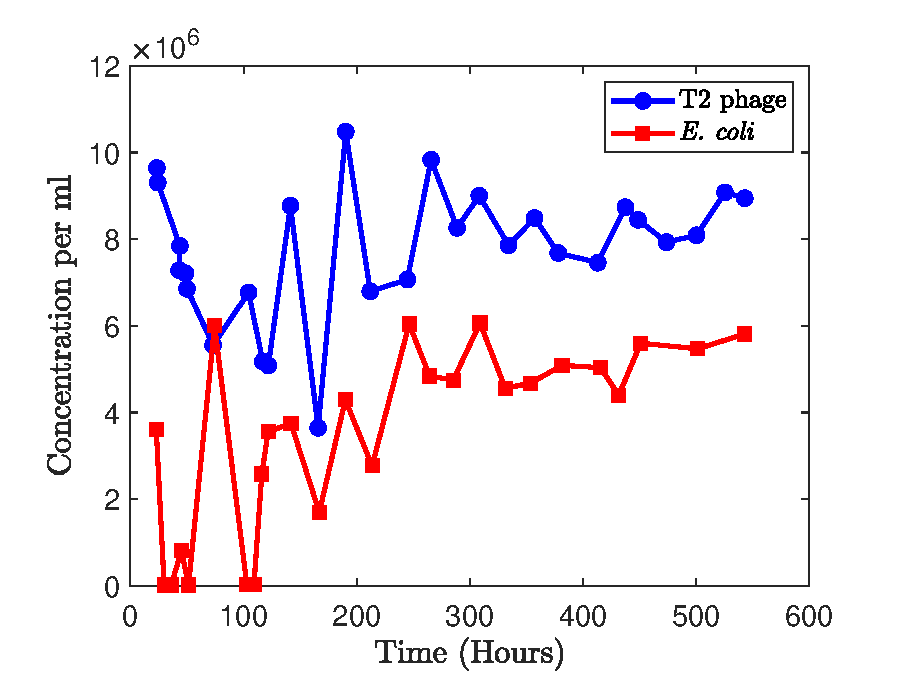
\includegraphics[scale=0.55]{L3.eps}
\subcaption[subfigcapskip = 50pt]{Density of glucose-limited populations with a T2-sensitive strain of \textit{E. coli} B and the bacteriophage T2.}

\end{subfigure}\hfill
\begin{subfigure}[t]{0.45\textwidth}
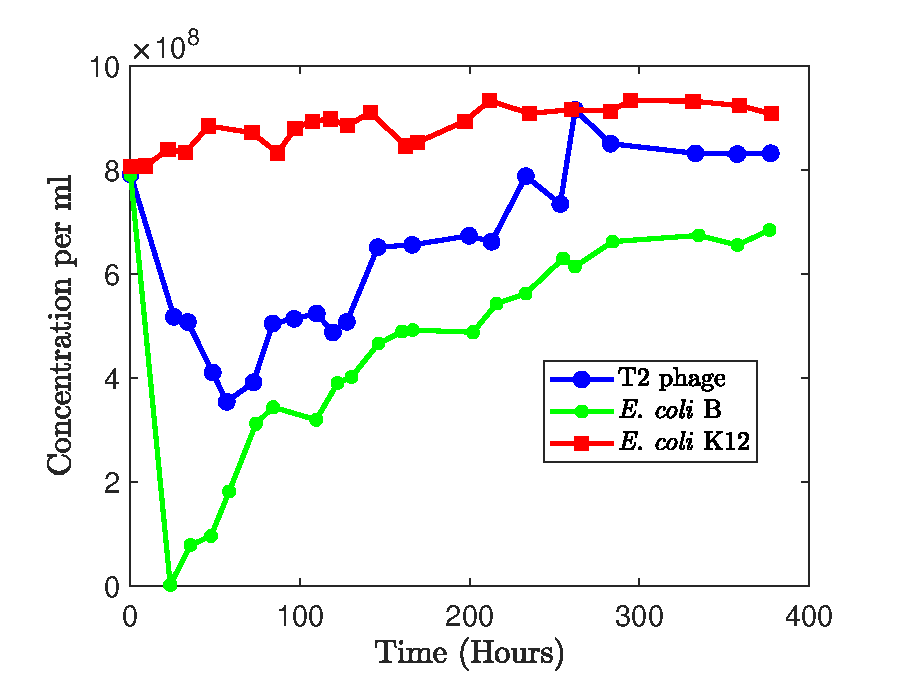
\includegraphics[scale=0.55]{L4.eps}
\subcaption[subfigcapskip = 50pt]{Glucose-limited continuous culture populations with a T2-sensitive strain of \textit{E. coli} B, a T2-resistant strain of \textit{E. coli} K12, and the bacteriophage T2.}
\end{subfigure}\hfill
\caption[Population dynamics of sensitive, resistant bacteria and virulent phage.]{Population dynamics of sensitive, resistant bacteria and virulent phage. These data were extracted from Figure 5A and Figure 8 of Levin et al. (1977) \cite{levin_resource-limited_1977}, using PlotDigitizer.}
\label{fig:levin}
\end{figure}
\begin{figure}[t]
\captionsetup[subfigure]{labelformat=empty}
\centering
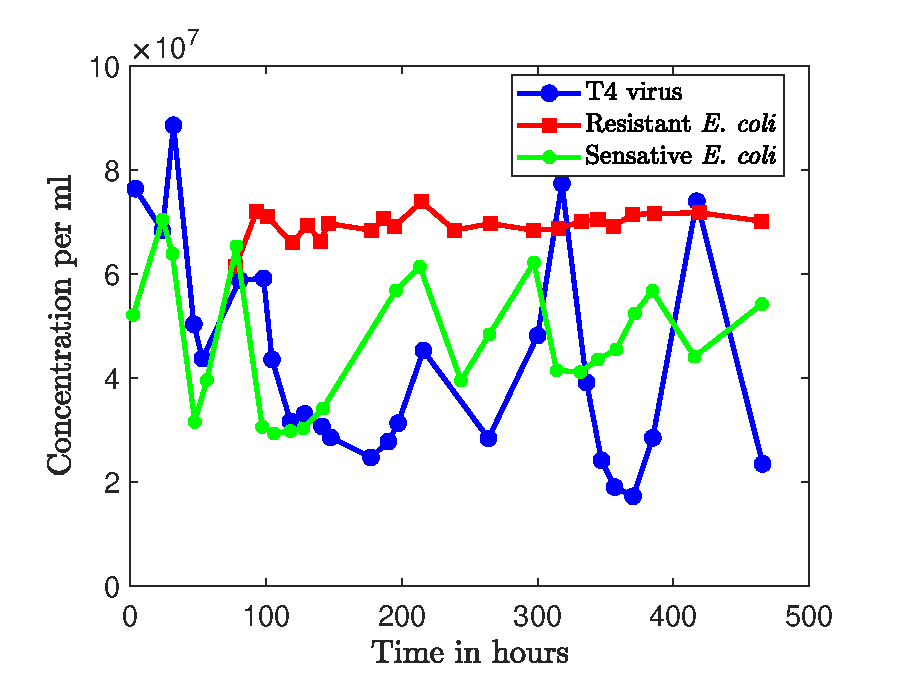
\includegraphics[scale=0.65]{L1.eps}
\caption[Dynamics of \textit{E. coli} and bacteriophage showing oscillating dynamics.]{Dynamics of T4 sensitive \textit{Escherichia coli} (green), T4 resistant \textit{Eschericia coli} (red), and bacteriophage T4 (blue) in chemostats supplied with media containing glucose, showing oscillating dynamics. Resistant \textit{E. coli} emerges approximately after 78 hours. The population of T4 phage and sensitive bacteria oscillate. The data was extracted from Figure 2B of Bohannan et al. (1999)  \cite{bohannan_effect_1999} using PlotDigitizer. }
\label{fig:levin2}
\end{figure}

In the Lotka-Volterra model, introduced by Lotka in 1925 \cite{lotka_elements_1925} and Volterra in 1926 \cite{volterra_variations_1928}, the consumption of prey follows the law of mass action, i.e. the consumption of prey by a predator is proportional to the product of the population density of predator and prey. The prey population grows exponentially in the absence of a predator, and the predator population declines exponentially in the absence of the prey.  The associated system of differential equations:   
\begin{eqnarray}\label{L-V}
\frac{dx}{dt} & =& r x - g x y \nonumber\\
\frac{dy}{dt} & = & \gamma g x y - \mu  y
\end{eqnarray}
gives the classical Lotka-Volterra model.  Here, $x$ corresponds to the population density of the prey, $y$ corresponds to the population density of predator, $r$ is the rate of increase of prey population, $g$ is the predation rate, $\gamma$ is the reproduction rate of predators and $\mu$ is the mortality rate of predators. With appropriate parameter values, this model predicts the coexistence of predator and prey, see Figure~\ref{fig:lotka}.

\begin{figure}[t]
\captionsetup[subfigure]{labelformat=empty}
\centering
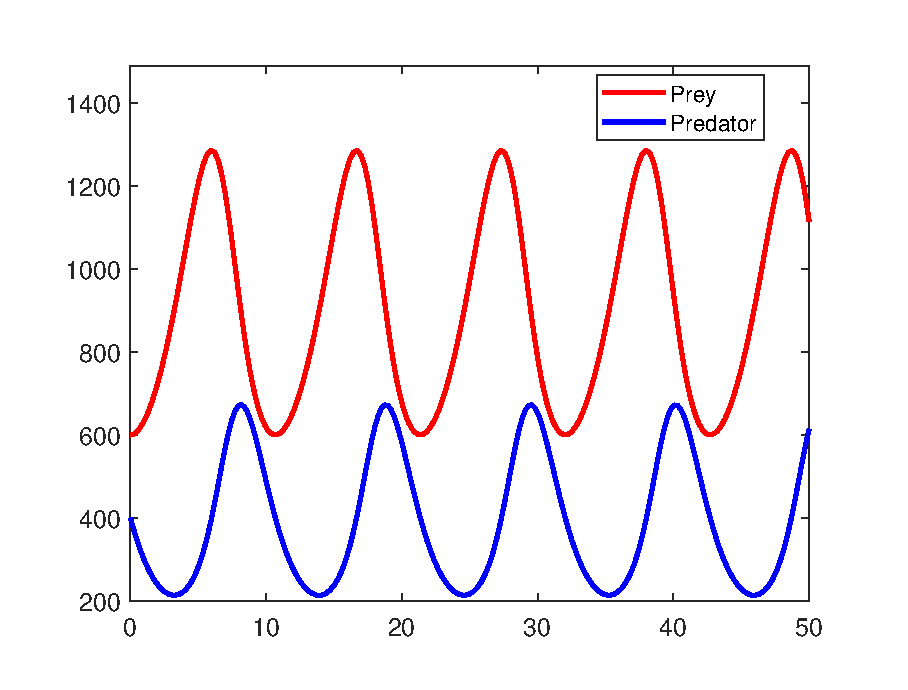
\includegraphics[scale=0.65]{lotka.eps}
\caption{Lotka-Volterra model showing long-term existence of both predator and prey populations.}
\label{fig:lotka}
\end{figure}

This model has been further improved, for example, by introducing a logistic growth term $r (1-\frac{x}{K})$, where $K$ is the carrying capacity of the prey population, instead of the exponential growth term $r x$ \cite{nisbet_modelling_1982}.  The linear functional response $ \mathcal{F}(x) =  g \,x$ in System \ref{L-V}, called the Holling Type I response, can also be replaced by more realistic functional responses (Holling Type II, Holling Type III and Holling Type IV) \citep{dawes_derivation_2013}.   

Based on the nature of the interaction between phages and bacteria and the qualitative behaviour of such predator-prey models, predator-prey type models were the natural choice for modelling the interaction between phages and bacteria. In 1961 Campbell \cite{campbell_conditions_1961} presented the following model 
\begin{eqnarray}\label{Camp}
\frac{dB}{dt} & =& r_{B} B \left(1-\frac{B}{K}\right) - aB -  k PB \nonumber\\
\frac{dP}{dt} &=& k b B(t-l) P(t-l) - k BP - a P - d P ,
\end{eqnarray}
where $B$ and $P$ are population densities of bacteria and free phages, respectively. The parameters $r_B$, $a$, $k$, $d$ represent the growth rate of bacteria, the flow rate constant, the absorption rate and the rate of spontaneous inactivation of phages, respectively.  Each infected bacterial cell yields $b$ phage particles (burst size) at a time $l$ seconds after infection. The author performed a local steady-state analysis of this model, concluding that phages will maintain bacteria at a low but non-zero level if they grow rapidly; otherwise phages will die out. In System \ref{Camp}, the functional response is $\mathcal{F} = k B$. 

Building on the Campbell model and to account for the relationship between prey growth and the availability of resources, a chemostat model with constant inflow of nutrient solution and outflow of culture was proposed by Levin et al. in 1977 \cite{levin_resource-limited_1977}. Multiple resources and multiple species of bacteria and phages were considered. Therefore, phages compete in addition to bacterial competition. The behaviour of the model developed was compared with that of experimental populations of \textit{E. coli} and its virulent virus T2, see Figure~\ref{fig:levin}. 

Campbell did not discuss the stability analysis at all, whereas Levin et al. investigated the model by integrating the equations numerically but did not carry out stability analysis analytically. Bremermann \cite{bremermann_parasites_1983} presented a relatively simpler model by assuming that time delays were negligible on the timescale of consideration. He did not use delay differential equations. If  $S$ denotes the density of susceptible hosts, $I$ denotes the density of infected hosts and $P$ the density of phages, then the equations for this model are given as:
\begin{eqnarray}\label{Br}
\frac{dS}{dt} &=& r_s S \left(1- \frac{S}{K}\right) - \beta S P \nonumber\\
\frac{dI}{dt} &=& \beta S P - \lambda I \nonumber\\
\frac{dP}{dt} &=& b I - \mu P.
\end{eqnarray}
Here $r_s$ is the bacterial growth rate, $K$ is its carrying capacity, $\beta$ is the rate of adsorption, $\lambda$ is the death rate of infected bacterial hosts, $b$ is the rate at which new phages are produced (burst size) and $\mu$ is the death rate of phages.  By carrying out stability analysis of  system \ref{Br} the author was able to show that the existence of phages depends on the carrying capacity of the bacteria, $K$. If the carrying capacity falls below a certain threshold $\left( \frac{\lambda\, \mu}{b\, \beta}\right)$ the phage population and infected hosts will die out and they uninfected host population will approach its carrying capacity $K$.  

Later, several authors modified the above models. For example Lenski et al. \cite{lenski_constraints_1985} included mutational events into the Levin et al. model \cite{levin_resource-limited_1977}. These authors also compared model predictions with the results of experiments with \textit{E. coli} and virulent phage and the evolutionary constraints for \textit{E. coli} and virulent phage.  In 1997, Bohannan and Lenski \cite{bohannan_effect_1997} model was a modification of the Levin model. This model ignored the dynamics of infected cells by considering them to instantaneously become dead. The authors solved the model analytically and examined the behaviour of the system numerically. The dynamics of the T4 and \textit{E. coli} populations were also shown, see Figure~\ref{fig:levin2}. A model, similar to Bremermann's model, was proposed by Beretta and Kaung  in 1998 \cite{beretta_modeling_1998} for marine bacteriophages. A rich literature about phage-bacteria interactions is now available, for detail see \cite{payne_understanding_2001, gourley_delay_2004, smith_models_2008}.  

\section{Mobile genetic elements}
Mobile Genetic Elements (MGEs) are DNA segments that encode enzymes or other proteins that mediate DNA movements within genomes or between bacterial cells \cite{frost_mobile_2005}. MGEs are involved in all aspects of genome organization, function, and evolution \cite{craig_mobile_2015, arkhipova_mobile_2016}. Horizontal gene transfer (HGT) is the intercellular movement of DNA that allows transfer of genes from one bacterium (donor) to another bacterium (recipient) by means other than vertical transmission. This transfer of genetic material can take place through: (1) transformation, where bacteria take DNA from their environment; (2) conjugation, where DNA is exchanged between two bacteria; or (3) transduction, which is bacteriophage-mediated exchange of genetic material between two bacteria \cite{soucy_horizontal_2015}. 
The role of HGT in bacterial evolution has long been recognised \cite{huddleston_horizontal_2014, soucy_horizontal_2015}.   
\subsection{Overview of mobile genetic elements}
The discovery of MGEs is attributed to McClintock for her work on the maize chromosome, where the existence of jumping genes in maize chromosomes was reported \cite{mcclintock_origin_1950}. The genomes of both prokaryotes and eukaryotes carry abundant MGEs \cite {schnable_b73_2009, lynch_origins_2007}. In this investigation, we will focus only on MGEs in prokaryotic genomes.  

MGEs can be categorized into different classes; we outline four important classes here. 
(1) Bacteriophages (lytic/lysogenic/prophages) are one of the most important classes of MGEs which help bacterial cells to exchange genetic material with each other through HGT \cite{ canchaya_phage_2003}. (2) Plasmids are extra-chromosomal genetic material and are very common in bacterial genomes \cite{ phillips_plasmid_2004}. Plasmids are transformed from donor bacterium to recipient bacterium through conjugation, a form of horizontal gene transfer in which bacteria exchange genetic material directly \cite{ phillips_plasmid_2004}.  Plasmids usually carry genes that bring genotypic changes to its bacterial host, for example, antibiotic resistance genes \cite{ svara_evolution_2011}.   
(3) Transposable elements (TEs) are ubiquitous DNA sequences in bacterial genomes that move within their host bacterial genome \cite{ garrido-ramos_evolutionary_2012}. 
(4) Insertion sequences (ISs), a type of TE \cite{capy_dynamics_1998}, are the simplest of MGEs and can move around within genomes or horizontally as a part of other MGEs \cite{ vandecraen_impact_2017}.

 \subsection{Evolutionary forces affecting mobile genetic elements}
 
 Mobile genetic elements are either intracellular (inserted from within the cell) or intercellular (inserted from another cell) and are typcically considered to be genetic parasites or junk DNA. The insertion of these new genetic materials comes with some cost to the bacterial host. The cost incurred by these MGEs to the host varies significantly and depends on the nature of the inserted element. Bacteriophages kill their host to release progeny virions but other mobile genetic elements like plasmids or TEs do not kill their host cell. However, to maintain these elements in its genome the host bacteria must exert some extra energy, making them costly \cite{diaz_ricci_plasmid_2000}.  These MGEs can also disrupt important functions by disrupting a bacterial gene upon insertion \cite{simser_novel_2005, naito_role_2016}.

On the other hand, these inserted genetic materials can also endow some benefits to their bacterial host by carrying genes that are beneficial to the host \cite{vandecraen_impact_2017}. Frost et al., in \cite{frost_mobile_2005}, called mobile genetic elements  ``the agents of open source evolution". 
Mobile genetic elements may also have a positive impact on the bacterial host’s neighbours by producing proteins that are beneficial for neighbours \cite{livermore_beta-lactamases_1995} or a negative impact by producing proteins that harm the host’s neighbours \cite{dykes_selection_1997}.  The relationship between mobile genetic elements and their host and host’s neighbours is further explained by  Rankin et al. in \cite{rankin_what_2011}.
 
 Once inserted into the bacterial genome, MGEs are faced with several evolutionary forces:
 
 (1) The rate of insertion of these MGEs into the bacterial genome is an important factor in determining their future distribution in the host population. For example, an important factor in determining the prophage distribution in bacterial genomes is the lysogeny \cite{bobay_pervasive_2014}, the integration of the phage genome with the bacterial genome after it enters into the bacterial cell.
 
(2) Mutation occurs randomly and is a change in the nucleotide sequence of a short region of a genome. Mutation is considered to be an important force in shaping bacterial genome evolution \cite{hershberg_mutationengine_2015}. It has been shown that mutation in the bacterial genome is biased toward deletion \cite{kuo_deletional_2009}.  Mutations have important and profound affects on these MGEs, for example, mutation can impair genes required for the excision of prophage from a bacterial genome, resulting in domestication of these prophages in bacterial genomes \cite{casjens_prophages_2003, wang_cryptic_2010}.

(3) MGEs, inserted into bacterial genomes, are part of the bacterial host genome and are transmitted vertically from parent to offspring. If these MGEs contain genes that can help its host to proliferate this will, in turn, help these MGEs to proliferate in the host population. 

(4) Many MGEs have the ability to invade host genomes horizontally. As described before, this horizontal transfer of genes between bacterial genomes is considered to be a very important factor in the evolution of bacterial genomes and may occur through conjugation, transformation or transduction  \cite{soucy_horizontal_2015}.

(5) MGEs usually have a stable relationship with their host's genome and are transmitted vertically as a part of the bacterial genome to the daughter cells. However some MGEs, like prophages, can excise from the bacterial genome, in response to environmental signals or spontaneously, and kill the host bacterium \cite{lopez_induction_2014}. 

\subsection{Mathematical modelling of mobile genetic elements}
Since the discovery of mobile genetic elements there have been many theoretical approaches to explain the nature of these DNA segments. Most of these approaches deal with a particular class of MGEs. The initial mathematical models of MGEs were mostly focused on understanding the mechanisms that prevent the unlimited expansion of MGEs in host populations, despite their tendency for proliferation. These studies also focused on obtaining the equilibrium copy number distribution under diverse evolutionary scenarios. Below we provide some overview of these models aimed at the evolution of MGEs in prokaryotic genomes.

Stewart and Levin, in 1977, developed an ODE model for the population dynamics of horizontally transmitted plasmids in bacterial genomes \cite{ stewart_population_1977} and argued that plasmids could not persist if there is a low rate of HGT. They also argued that if plasmids persist, then cells carrying them will maintain high frequencies in bacterial populations, even if the cells carrying them are less fit. In 1980, Levin and Stewart presented an ODE model for the population dynamics of nonconjugative plasmids \cite{levin_population_1980}. Here they concluded that nonconjugative plasmids could be maintained even when the bacteria carrying them have a lower reproduction rate than other bacteria and it is highly unlikely that they will be maintained without conferring to the host some selective benefit. The above mentioned models assume that random encounters occur between members of the plasmid-bearing population and plasmid-free population, at a rate that is proportional to the densities of these populations, that is, the law of mass action. Several variants of these models were presented over the years, for details see \cite{freter_experimental_1983, lundquist_transitory_1986, zhong_accounting_2010, turner_tradeoff_1998}. To capture the dynamics of the plasmid in spatially structured habitats other techniques have been applied, for example, computational models \cite{ krone_modelling_2007, lagido_model_2003, ponciano_population_2007, merkey_growth_2011, connelly_modeling_2011}.

The evolution of TEs in prokaryotic genomes has been studied by many authors \cite{hartl_why_1988, basten_branching-process_1991, moody_branching_1988, dolgin_fate_2006, wagner_cooperation_2006, drakos_extinction_2015, rabbani_dynamics_2016}. All these authors used the branching process method to study the evolution
of TEs in prokaryotic genomes.  In a Markov process the outcome of a state is independent of past states and depends only on the present state.  A branching process is a special type of Markov process. Using these methods, Sawyer and Hartl, in 1986, developed a model for the distribution of TEs in prokaryotic genomes \cite{sawyer_distribution_1986}. The model assumed that TEs are entering prokaryotic genomes at a constant rate and can reduce the fitness of the host in proportion to their numbers in the host genome. A model in which the TEs can convey a selective advantage to the host was also considered. The equilibrium distributions of copy numbers for these models were determined. Relevant parameters were estimated using data regarding the distribution of insertion sequences in natural isolates of \textit{Escherichia coli}. In another study, Hartl and Sawyer (1988) used a branching process to model the insertion sequences in \textit{E. coli} and concluded that horizontal gene transfer is essential in maintaining bacterial insertion sequences \cite{hartl_why_1988}. 

Basten and Moody formulated a model to analyze the spread of transposable genetic elements in prokaryotic genomes, in 1991 \cite{basten_branching-process_1991}.  The authors incorporated selection, transposition and deletion in their model. They concluded that TEs can spread through a population despite selection against them. In \cite{edwards_transiently_2003}, the effect of  a fluctuating environment on the spread and persistence of TEs was studied.  

Van Passel et al. developed a birth–death–diversification model for mobile genetic elements subject to sequence diversification \cite{van_passel_birth_2014}. They applied the model to putative mobile promoters, a type of MGE,  and quantified the relative importance of duplication, loss, horizontal gene transfer (HGT), and diversification to the maintenance of the PMP reservoir.

Finally, in 2018, Iranzo and Koonin developed an ODE model and carried out comparative genomic study to explain the roles of selection, horizontal gene transfer, gene duplication and gene loss in the spread and persistence of MGEs \cite{iranzo_how_2018}. By quantifying the fitness of MGEs to the bacterial hosts they showed that these MGEs are deleterious at evolutionary timescales and characterized them as parasites. 

\section{Motivation and outline of the thesis}
Due to the alarming spread of antibiotic resistance and its consequences to public health, the evolution of antibiotic resistance genes has been a topic of interest for many scientists \cite{ hong_comprehensive_2018}. Experimental results have shown that the synergistic use of antibiotics and phages has a promising effect against antibiotic resistance bacteria, especially those in biofilms \cite{chaudhry_synergy_2017}. In \textbf{Chapter 2}, we have developed an ODE model to study the effect of antibiotics and phages on the bacterial population in a biofilm. We have exploited the idea of a group defense mechanism by assuming that as the biofilm becomes more and more mature, the harder it becomes for phages to kill bacteria in the biofilm colony. Here we show that the synergistic use of phages and antibiotics, especially using phages first and then antibiotics, can incur maximum damage to the biofilm bacteria. We also show that neither phages nor antibiotics, alone,  can eliminate the biofilm completely. Complete elimination of biofilm bacteria is possible only if we could stop the further attachment of planktonic bacteria to the biofilm colony.

The advent of modern technologies has resulted in huge databases about MGEs and has opened new ways to investigate the evolution of MGEs and their role in the evolution of bacteria. Although a substantial literature is available about the evolution of MGEs, these studies are lacking the evolution of an important player responsible for the evolution of bacterial genomes and hence antibiotic resistance genes, the prophages. In \textbf{Chapter 3} we attempted fill this void. Here, we have developed a PDE model to mimic the prophage size distribution in bacterial genomes. The basic question we investigate here is \textit{``Why is the prophage size distribution in bacterial genomes bimodal?"} We fitted our PDE model to the three publicly available data sets and were able to quantify various evolutionary forces acting on prophages. 

The next question we investigated is \textit{``Which genes are enriched in defective prophages?".} In \textbf{Chapter 4}, we study the genetic repertoire of prophages, especially, which genes are enriched in defective prophages. We downloaded data describing prophages in two well-studied data sets from GenBank and examine their genetic repertoires. Here we developed an ODE model to investigate possible steady states of prophages genes. We also developed a gene-level model to get more insight into the genetic repertoire of prophages. 

In \textbf{Chapter 5}, we present conclusions and possible future work.  

\addcontentsline{toc}{chapter}{Bibliography}
\bibliographystyle{abbrv}
\bibliography{refrence}


\chapter{Phage therapy and antibiotics for biofilm eradication: a predictive model}
%\abstract{
Bacteria that make up the complex physical structures known as biofilms can be 10-1000 fold more resistant to antibiotics than planktonic (free-living) bacteria.  In this chapter we develop a mathematical model to analyze therapeutic techniques that have been proposed to reduce and/or eradicate biofilms, specifically, antibiotics and phage therapy. In this context, the biofilm can be understood as a group defense mechanism, such that the functional response of phages to the biofilm bacterial density is reduced as the biofilm approaches carrying capacity. To capture this mechanism we introduce the function $f(x)=\left(\kappa-\frac{x}{K}\right)x,$ where $x$ is biofilm density, $K$ is biofilm carrying capacity and $1<\kappa <2$ is the group defense parameter. The model predicts that two therapeutic strategies of recent experimental interest (phage therapy followed by antibiotics, or antibiotics followed by phage therapy) can reduce but not eradicate the biofilm.  In contrast, we predict that complete elimination of biofilm bacteria can be achieved by mechanisms that block the attachment of planktonic bacteria to the biofilm.
%}
\section{Introduction}
Bacteria are ubiquitous unicellular organisms, with critical importance in both human health and disease \citep{abedon_bacteriophage_2008}. Bacteria can exist as planktonic (free-living) cells, or in complex communities known as biofilms.  In the biofilm state, the bacterial colony is attached to a surface; within the biofilm each cell is sessile and surrounded by extracellular polymeric substances (EPS), substances produced by bacteria in the colony that determine the physical and chemical properties of the biofilm \citep{harper_bacteriophages_2014}. Biofilms are responsible for a variety of problems in water distribution systems \citep{douterelo_dynamics_2016}, the food industry \citep{van_houdt_biofilm_2010}, and medical treatment \citep{omar_microbial_2017, ciofu_antibiotic_2017}.  Most importantly, biofilms have been implicated as a key factor in two-thirds of human infections \citep{fux_bacterial_2003}. \\

Bacteria are able to rapidly develop resistance against agents employed to eradicate them. %This resistance may be genotypic, phenotypic or a combination of both.  Genotypic resistance is inherited resistance through changes to the genetic code, while phenotypic resistance is due to a change in the phenotype (current physical characteristics) of the bacterial cell. One of the most important causes of phenotypic resistance is the physical structure of bacterial population \citep{sanchez-romero_contribution_2014}, called biofilm. 
In particular, bacteria in a biofilm have been shown to increase resistance to antibiotics by factors of ten to 1000 \citep{davies_understanding_2003}. Amongst the reasons for enhanced resistance in the biofilm state is the EPS structure surrounding the biofilm colony, which can completely block the infiltration of antibiotics, and the presence of persister cells in the biofilm colony, which are in a metabolically inactive state and thus protected from antibiotic action \citep{davies_understanding_2003}.\\

The goal of reducing or eradicating biofilm populations has been the focus of research over many years, and there has been much experimental work in this regard \citep{fleming_approaches_2017, ciofu_antibiotic_2017, feng_bacterial_2015}. Many agents have been employed for this purpose, which include but are not limited to natural inhibitors of biofilm, for example honey \citep{lee_low_2011}, %jakobsen_ajoene_2012}, 
drugs (antibiotics, biofilm-degrading components) \citep{lynch_new_2010, mu_potent_2016}, bacteriophages and phage-derived enzymes \citep{azeredo_use_2008, fernandez_low-level_2017, abedon_ecology_2015} or combinations of some of these \citep{chaudhry_synergy_2017}.  While phage therapy has been proposed as possibly the most effective of these agents, phages alone may not be sufficient to completely eradicate a biofilm\citep{abedon_ecology_2015}. Most recently, experimental work demonstrated that
%was carried out to investigate the question ``How does one deal with the increasing frequency of pathogens that are genetically resistant to multiple antibiotics and phenotypically resistant because of the physical  structure of their population?" \citep{chaudhry_synergy_2017}. They used some therapeutic strategies to overcome the resistance. They claimed 
using phage therapy first, followed by antibiotics, maximized the killing of bacteria in an established biofilm.\\

In this chapter, we develop a mathematical model to study these therapeutic strategies in detail.  In section 2.2, we develop the model, tracking biofilm and planktonic bacteria in two linked compartments. In section 2.3, we explore therapeutic strategies including: phage followed by antibiotics; antibiotics followed by phage; and a novel strategy we propose which may have the potential to eradicate the biofilm. In section 2.4, we derive some conclusions from our analysis.

\section{Mathematical model}

We model the interaction between bacteria and bacteriophages (viruses that infect bacteria) using an established predator-prey approach \citep{lenski_dynamics_1988}. %For this purpose we divide bacteria into biofilm and planktonic compartments.  
Our model considers cells of a single bacterial species in either a biofilm or planktonic compartment.   The model studies the population dynamics of biofilm cells, $B$, planktonic cells, $P$ and phage, $V_B$ and $V_P$, in the biofilm and planktonic compartments respectively.  The parameters of the model are described as follows.\\
 
The bacterial populations (biofilm or planktonic) are modeled as cell densities per unit volume, cells/cm$^3$. The biofilm population can increase logistically with a maximum growth rate $r$, but is limited by a fixed number of available attachment sites in the biofilm matrix, given by carrying capacity $K_{B}$ cells/cm$^3$.  Similarly,  planktonic bacteria can grow logistically with maximum growth rate $r$ but are limited by carrying capacity $K_P$. The planktonic bacteria join the biofilm at rate $\mathcal{A}(B,P)$ and biofilm bacteria leave the biofilm with detachment rate $\mathcal{D}(B,P)$. It has been shown that T4 can diffuse fairly through biofilm channels \citep{doolittle_tracing_1996}; in the model, phages enter the biofilm compartment at rate $p$ and leave at rate $q$. In addition, as described above, bacteria in a mature biofilm present substantial resistance to bacteriophages. The expression $f(B)\,V_B$ gives the number of adsorption events per unit time in the biofilm, where $f(B)$, the phage response function, will model this group defense mechanism. The number of adsorption events per unit time in the planktonic compartment is given by $g(P)\,V_{P},$ where $g(P)$ is the phage response function in the absence of group defense. We neglect the time delay between infection and lysis and assume that each adsorption event instantaneously produces $b$ daughter phages, resulting in new $b f(B)\,V_{B}$ and $b\,g(P)\,V_{P}$ bacteriophages in the biofilm and planktonic compartments respectively. Bacteriophage are cleared or denatured at rate $c$. 
These assumptions yield the following system:
\begin{eqnarray}\label{modelb}
\frac{dB}{dt} &=& r\left(1-\frac{B}{K_{B}}\right)B-f(B) V_{B} +\mathcal{A}(P,B)-\mathcal{D}(B,P)\nonumber\\
\frac{dP}{dt} &=& r\left(1-\frac{P}{K_{P}}\right)P- g(P)V_{P}-\mathcal{A}(P,B)+\mathcal{D}(P,B)\nonumber\\
\frac{d V_{B}}{dt} &=& bf(B)V_{B}-cV_{B}+p V_{P}-qV_{B}\nonumber\\
\frac{d V_{P}}{dt} &=& bg(P)V_{P}-cV_{P}+q V_{B}-p V_{P}.
\end{eqnarray}
We note that the attachment and detachment rates, $\mathcal{A}(B,P)$ and $\mathcal{D}(B,P)$, satisfy $\mathcal{A}(B,0)=0$ and $\mathcal{D}(0,P)=0$.
More generally, system \ref{modelb} can also be considered as a two-patch predator-prey model, with group defense acting in one patch only, as illustrated in Figure~\ref{fig:patches}. 
%Prey can take refuge from predators in patch-$2$, where they form their colony to have a group defense mechanism against any foreign invader. But this group defense mechanism is not perfect and still predator can infiltrate with some rate into patch-$2.$   Our model reduces to predator-prey system with group defense and without group defense if we consider only patch-$1$ or patch-$2$, respectively.
\begin{figure}[ht]
\centering
 \resizebox {80mm} {!}{
\begin{tikzpicture}[thick]
\draw [red, dashed,line width=1pt, shade, 
            outer color= blue!15!white, inner color=white, 
            align=center](-0.8,2) ellipse (3.5cm and 5.5cm);
\draw  [shade, outer color= black!5!white, inner color=white, 
            align=center](-3,-2) -- (1.5,-2) -- (1.5,6)-- (-3,6)--cycle;
\draw [shade, outer color= purple!70!white, inner color=white, 
            align=center](-0.5,4) circle  (1.5cm);
\draw [shade, outer color= red!50!white, inner color=white, 
            align=center](-0.5,0) circle  (0.8cm);
\draw [shade, outer color= black!5!white, inner color=white, 
            align=center](6,-2) -- (11,-2) -- (11,6)-- (6,6)--cycle;
\draw [shade, outer color= purple!70!white, inner color=white, 
            align=center](8.2,4) circle  (1.5cm);
\draw [shade, outer color= red!50!white, inner color=white, 
            align=center](8.2,0) circle  (0.8cm);
\node (a) at (-0.3,4) {\Huge $ B$};
\node (b) at (-0.5,0) {\Huge $ V_{B}$};
\node (c) at (8.2,4) {\Huge $ P $};
\node (d) at (8.2,0) {\Huge $V_P$};
\draw [->, line width =2pt]  (7, 5.1).. controls (4,6) .. (0.6,5.1);
\node (e) at (4,6.3) {\Huge ${\LARGE {\mathcal{A}(B,P)}}$};
\draw [->, line width = 2pt]  (0.6,2.9).. controls (4,2) ..(7, 2.9) ;
\node (f) at (4.3,2.99) {\Huge $\mathcal{D}(B,P)$};
\draw [->, line width =2pt]  (8, 0.9).. controls (4,2) .. (0.1,0.9);
\draw [->, line width =2 pt]  (0.1,-1.0).. controls (4,-2) .. (8, -1.0);
\draw [->, line width = 2pt]  (-1, 4).. controls (-1.5,2.3) .. (-1,0.7);
\draw [->, line width = 2pt]  (9.2, 4).. controls (9.5,2.3) .. (9.2,0.3);
\node (g) at (4,1.2) {\Huge $p$};
\node (h) at (4,-1.2) {\Huge $q$};
\node (i) at (-0.8,-4) {\LARGE Biofilm bacteria};
\node (i) at (-0.8,8) {\LARGE Patch-2};
\node (j) at (8.5, -4) {\LARGE Planktonic bacteria};
\node (i) at (8,8) {\LARGE Patch-1};
\node[label={[label distance=0.5cm,text depth=-1ex,rotate=90]right:\Huge $bf(B)$}] at (-2.4,-0.1) {};
\node[label={[label distance=0.5cm,text depth=-1ex,rotate=90]right:\Huge $ bg(P)$}] at (9.9,-0.1) {};
\node[label={[label distance=0.5cm,text depth=-1ex,rotate=90]right: {\LARGE EPS structure in biofilm (protective layer).}}] at (-5.5,-3.5) {};
\end{tikzpicture}
}
\caption[Diagram of the model.]{Diagram of the model. In patch-$1$ there is no group defence mechanism but prey (bacteria) can take refuge in patch-$2,$ where they can have group defence mechanism and can protect themselves against predator (phage).}\label{fig:patches}
\end{figure}\\

%In next section analysis of recently employed therapeutic strategies is carried out and is shown that although these therapeutic strategies can maximize the killing of bacteria in biofilm but can  not results in complete eradication of biofilm. We also suggest a therapeutic strategy which can result in complete eradication of biofilm and if there is no inherited resistance complete elimination of bacteria is possible. 

\section{Therapeutic strategies}
Recent experimental work has addressed approaches for minimizing or eradicating bacterial biofilms \citep{chaudhry_synergy_2017}.  In particular, Chaudhry {\it et al.} compared two therapeutic strategies: applying antibiotics and then phages, or applying the same two agents in the reverse order.  Treatment with phages first followed by antibiotics resulted in maximum killing of biofilm bacteria. Here we predict that although these strategies can indeed reduce the biofilm, neither strategy can eradicate the biofilm completely.

\subsection{Using antibiotics first and then phages}

Given that planktonic bacteria are many-fold more sensitive to antibiotics than biofilm bacteria, we assume that an appropriate antibiotic is administered such that planktonic bacteria can be effectively eliminated before phage therapy. We also assume that $\mathcal{A}(B,P)=\mathcal{D}(B, P).$ After the application of antibiotic we will arrive at the following system 
\begin{eqnarray}\label{modelb1}
\frac{dB}{dt} &=& r\left(1-\frac{B}{K_{B}}\right)B-f(B) V_{B} \nonumber\\
\frac{d V_{B}}{dt} &=& bf(B)V_{B}-cV_{B}.
\end{eqnarray}
This is a standard predator-prey system with group defense, as studied in  \citep{wolkowicz_bifurcation_1988, freedman_predator-prey_1986, zhu_bifurcation_2002,broer_predator-prey_2006}. In particular,   $f(B)$ must satisfy $f(0)=0, \, f(B)>0 \,\, \text{for all}\,\, B>0$, and if there exists a constant $M>0,$ such that 
$f^{'}(B)>0\,\, \text{if}\,\, B<M\, \, \text{and} \,\,f^{'}(B)<0 \,\, \text{if}\,\, B>M$, then the system models group defence \citep{freedman_predator-prey_1986}.
The  function $f(B)=\frac{m\,B}{\alpha \, B^{2}+ \beta \, B+1},$
called the Holling Type-IV or the Monod-Haldane function, was introduced in \citep{andrews_mathematical_1968} and satisfies these properties. System (\ref{modelb1}) has been previously studied with the above functional response for $\beta >-2\sqrt{\alpha}$  \citep{zhu_bifurcation_2002, jiang_multistable_2017}, and with $f(B) = \alpha e^{ -\beta B}$ \citep{xiao_global_2001}.\\

In this study, we consider biofilm bacteria that cannot exceed their carrying capacity, such that $B \leq K_{B}$ at all times. Hence  we replace the property 
$f(B)>0 \,\, \text{for all} \,\,B>0$ by 
$f(B)>0 \,\, \text{for all} \,\,0<B\le K_{B}$ . 
%$f(B)>0 \,\, \text{for all} \,\,0<B<\kappa K_{B}, \,\, %\text{where} \,\, 1<\kappa<2.$
 To model this phenomenon, we propose a relatively simple functional response 
 $f(B)=\alpha\left(\kappa-\frac{B}{K_{B}}\right)B.$
\textcolor{black}{The rationale for this function is similar to the rationale underpinning logistic growth: we assume that as the biofilm population
 approaches carrying capacity, the ability of phage to
 penetrate the biofilm is reduced, linearly.} The resulting functional response has the same properties as that of $f(B)$ defined in \citep{zhu_bifurcation_2002,xiao_global_2001} for $0<B \leq K_{B}$. 
 Here $\alpha$ is proportional to the adsorption rate of phages to bacteria, $1<\kappa<2$ is the group defense parameter, and $K_{B}$ is the carrying capacity of the biofilm bacteria. A convenient feature of this model is that the group defense mechanism can be controlled through the parameter $\kappa$; $\kappa=1$ corresponds to a perfect group defense mechanism \textcolor{black}{(no phage adsorption when the biofilm is at carrying capacity)} and $\kappa=2$ corresponds to the absence of effective group defense \textcolor{black}{($f(B)$ increasing on $0<B\le K_B$ )}.\\  

System (\ref{modelb1}) has a maximum of four equilibria. Two boundary equilibria are: $E_{0}=(0,0),$ which represents the complete extinction of biofilm bacteria and phages; and $E_{K_{B}}=(K_{B},0),$ which represents the extinction of phages while the biofilm bacteria reaches carrying capacity. In addition, two positive equilibria are: $E_{\mu_{1}}=(\mu_{1}, \mathcal{F}(\mu_{1}))$ and $E_{\mu_{2}}=(\mu_{2}, \mathcal{F}(\mu_{2}))$ subject to some conditions of existence. Here 
$\mathcal{F}(B)=\frac{r\big(1-\frac{B}{K_{B}}\big)}{\alpha\big(\kappa-\frac{B}{K_{B}}\big)}$
and $\mu_{1}$ and $\mu_{2}$ are solutions to the equation $\hat{f}(B)=\hat{c},$
where $\hat{f}(B)=\left (\kappa-\frac{B}{K_{B}}\right)\,B$ and $\hat{c}= \frac{c}{b\, \alpha}$
and $\mu_{1}<\frac{\kappa \, K_{B}}{2}<\mu_{2} <K_{B}.$
The existence of the two positive equilibria $E_{\mu_{1}}$ and $E_{\mu_{2}}$ depend on the positioning of the prey isocline $V_{B}=\mathcal{F}(B)$ and predator isoclines $B=\mu_{1}$ and $B=\mu_{2}$. As we increase $\hat{c}$ in the interval $(0, \hat{c}_{M})$, $\mu_{1}$ and $\mu_{2}$ become closer to each other; when $\hat{c}=\hat{c}_{M}$ the two equilibria coincide and we get
$E_{\mu_{1}}=E_{\mu_{2}}=\left(\frac{\kappa \, K_{B}}{2}, \frac{r\left(1-\frac{\kappa}{2}\right)}{\alpha \left(\kappa-\frac{\kappa}{2}\right)}\right).$
Equilibria and their existence can be summarized in the following theorem.
\begin{theorem}
System (\ref{modelb1}) has four equilibria $E_{0},$ $E_{K_{B}},$ $E_{\mu_{1}}$ and $E_{\mu_{2}}$ if $\hat{c} \in (\hat{c}_{m}, \hat{c}_{M}),$ three equilibria $E_{0},$ $E_{K_{B}}$ and $E_{\mu_{1}}$ if $\hat{c} \in (0, \hat{c}_{m}),$ three  equilibria $E_{0},$ $E_{K_{B}}$ and $E_{\mu_{1}}=E_{\mu_{2}}=E_{\mu}=\left(\frac{\kappa \, K_{B}}{2}, \frac{r\left(1-\frac{\kappa}{2}\right)}{\alpha \left(\kappa-\frac{\kappa}{2}\right)}\right)$ if $\hat{c}=\hat{c}_{M},$ only two equilibria $E_{0}$ and $E_{K_{B}}$ if $\hat{c} > \hat{c}_{M},$
where $\hat{c}=\frac{c}{b\, \alpha},$ $\hat{c}_{M}=\frac{\kappa^{2}}{4}K_{B}$ and $\hat{c}_{m}= (\kappa-1)K_{B}.$
\end{theorem}

\subsubsection{Stability analysis}
It can be easily shown that $E_{0}=(0,0)$ has eigenvalues
$\lambda_{1}=r>0, \,\, \lambda_{2}=-c<0$
showing that $E_{0}=(0,0)$ is a saddle point. The equilibria $E_{K_{B}}=(K_{B},0)$ has
$\lambda_{1}=-r, \,\, \lambda_{2}=b\alpha(\hat{c}_{m}-\hat{c}),$ as eigenvalues, showing that $E_{K_{B}}$ is an attractive node, if $\hat{c}>\hat{c}_{m},$ and is a saddle point if $\hat{c}< \hat{c}_{m}.$ To study the stability of the other two equilibria, if they exist, we write the model (\ref{modelb1}) as
\begin{eqnarray}\label{modeb11}
\frac{dB}{dt} &=& f(B)\left(\mathcal{F}(B)- V_{B}\right)\nonumber\\
\frac{d V_{B}}{dt} &=& bf(B)V_{B}-cV_{B}.
\end{eqnarray}
The eigenvalues for $E_{\mu_{1}}$ are $\lambda_{1,2}=\frac{\xi_{1}\pm\sqrt{\xi_{1}^{2}-4\Delta_{1}}}{2},$ where
$\xi_{1}=f(\mu_{1})\mathcal{F}^{'}(\mu_{1})$
is the trace of Jacobian matrix of (\ref{modeb11}) at $E_{\mu_{1}}.$ Since $\mathcal{F}^{'}(B)<0,$ hence $\xi_{1}<0$ and 
$\Delta_{1} = b \, \alpha^{2}\, \mu_{1} \left(\kappa-\frac{\mu_{1}}{K_{B}}\right)\left(\kappa - \frac{2\, \mu_{1}}{K_{B}}\right)$
is the determinant of the Jacobian matrix at $E_{\mu_{1}}.$ As $\mu_{1}<\frac{\kappa K_{B}}{2},$ hence $\Delta_{1}>0.$ This demonstrates that $E_{\mu_{1}}$ is an attracting point. Similarly, the eigenvalues corresponding to $E_{\mu_{2}}$ are $\lambda_{1,2}=\frac{\xi_{2} \pm \sqrt{\xi_{2}^{2}-4\Delta_{2}}}{2},$
where $\xi_{2}=f(\mu_{2})\mathcal{F}^{'}(\mu_{2})<0$
is the trace of Jacobian matrix at $E_{\mu_{2}}$ and $\Delta_{2}= b \, \alpha^{2}\, \mu_{2} \left(\kappa-\frac{\mu_{2}}{K_{B}}\right)\left(\kappa - \frac{2\, \mu_{2}}{K_{B}}\right)<0$
is the determinant of the Jacobian matrix at $E_{\mu_{2}}.$ We conclude that $E_{\mu_{2}}$ is a saddle point.  Since only one equilibrium corresponds to the extinction of biofilm bacteria, and it is a saddle point for all feasible  parameter values, we conclude that complete eradication of the biofilm is not possible using this therapeutic strategy. {\color{black} This conclusion is consistent with the view, as discussed in an extensive review \citep{abedon_ecology_2015II}, that phage action is not sufficient for complete eradication of biofilms.}

\subsection{Using phages first and then antibiotics}
In order to understand phage therapy, we return to model (\ref{modelb}), approximating the complicated processes of attachment and detachment by simpler functions to gain tractability. Specifically, we assume biofilm bacteria detach at constant per capita rate $n$; \textcolor{black}{this
assumption has a long history in the literature, extending back to Freter's influential research on bacterial colonization of the intestinal tract \citep{freter_survival_1983,jones_freter_2003}.}  We further assume that planktonic bacteria attach at constant per capita rate $m$. \textcolor{black}{In Freter's original biofilm model, attachment is also proportional to the number of planktonic bacteria, but is further restricted by the number of available ``wall attachment sites'' \citep{freter_survival_1983}.  In our model, we restrict biofilm \emph{growth} by the number of attachment sites, $K_B$, but take a linear
attachment rate.} Since $B$ and $P$ are densities (cells per unit volume), the net transfer of cells between compartments must be scaled, yielding  $\mathcal{A}(B,P) = \left(\frac{vol_ {_{P}}}{vol_{_{B}}}\right)\, m\, P$ and $\mathcal{D}(B,P)=\left(\frac{vol_ {_{B}}}{vol_{_{P}}}\right)\, n\,B$, where $vol_B$  and $vol_P$ are the volumes of the biofilm and planktonic compartments respectively.  After the substitution of these function into system (\ref{modelb}), it can be shown by direct calculation that the resulting system has three equilibrium solutions: the trivial equilibrium, an equilibrium with both classes of bacteria only, and the all-existing equilibrium (exact expressions omitted for brevity).
%\begin{equation}\label{Eqn50}  
%\begin{array}{ll}  
%%{\rm E_0}: (B,P,V_B,V_P) = (0,0,0,0), \\
%{\rm E_1}: (B,P,V_B,V_P) = (B^{*}, P^{*}, 0, 0 ),\\
%{\rm E_2}: (B,P,V_B,V_P) = \big( %B^{**},P^{**},V_B^{**},V_P^{**} \big).
%\end{array} 
%\end{equation} 
%\subsubsection{Stability analysis}
Out of these equilibria the only equilibrium which corresponds to the complete eradication of biofilm bacteria is $\rm E_0.$ It can be shown by a direct calculation that this equilibrium $\rm E_0$ is a saddle point for all feasible parameter values. This demonstrates that phage therapy will not eradicate the biofilm.  Since the biofilm bacteria are resistant to antibiotics, we can conclude that even phage therapy followed by antibiotics will not remove the biofilm.

\subsection{A novel therapeutic strategy: blocking attachment}\label{3}
The model developed here allows us to address the following question: is there a therapeutic strategy, {\it in principle}, that could eradicate the biofilm?  Since attachment of planktonic bacteria is critical to biofilm maintenance, we investigated the model assuming this attachment is negligible, and phage therapy is also applied.
In this case it can be shown by direct calculations that system (\ref{modelb}), with the substitutions $\mathcal{A}(B,P)=0$ and $\mathcal{D}(B,P)=\left(\frac{vol_ {_{B}}}{vol_{_{P}}}\right)\, n\,B$, has five equilibrium solutions: 
\begin{equation}\label{Eqn52}  
\begin{array}{ll}  
{\rm E_0}: & (B,P,V_B,V_P) = (0,0,0,0) \\[0.5ex]  
{\rm E_1}: & (B,P,V_B,V_P) = (0,K_{P},0,0) \\[0.5ex]  
{\rm E_2}: & (B,P,V_B,V_P) = \big(0, 
\frac {c \left( c+p+q \right) }{\alpha\,b \left( c+q \right) }, 
\textstyle\frac{M\,p\, r} {b\alpha^2 (c+q)^2 K_P} 
 (\frac{vol_P}{vol_B}), \frac{M\,r}{b \alpha^2 K_P} 
\big),  \\[0.5ex]  
{\rm E_3}: & (B,P,V_B,V_P) = (B^*,P^*, 0, 0 ),  \\[0.5ex]  
{\rm E_4}: & (B,P,V_B,V_P) = \big( B^{**},P^{**},V_B^{**},V_P^{**} \big), 
\end{array} 
\end{equation} 
where 
\begin{equation}\label{Eqn3}  
M= b q \alpha K_P - c (c+p+q - b \alpha K_P) .
\end{equation}
Three of these equilibria, ${\rm E_{0}}, {\rm E_{1}}$ and ${\rm E_{2}}$, represent complete eradication of the biofilm. The equilibria ${\rm E_0}$ and ${\rm E_1}$ exist for any positive parameter values, while ${\rm E_2}$ exists only for $M \ge 0,$ i.e. $\alpha \ge \frac{c(c+p+q)}{b K_{P} (c+q)}.$ The equilibrium ${\rm E_{0}}$ is a saddle point for all feasible values of parameters. The equilibrium ${\rm E_{1}}$ is asymptotically stable if $n>r$ and $ \alpha <\frac{c\left(c+p+q\right)}{b\,K_{P}(c+q)}.$   This implies that if the detachment rate is greater than the birth rate of bacteria in the biofilm and adsorption rate is less than $\frac{c\left(c+p+q\right)}{b\,K_{P}(c+q)}$, then elimination of biofilm bacteria is possible; in particular, planktonic bacteria will reach their carrying capacity and there will be no biofilm or planktonic viruses.   Using the Hurwitz criterion, it can be shown that the equilibrium ${\rm E_2}$ is stable if $ M > 0 ,$  i.e. 
$\alpha >\frac{c\left(c+p+q\right)}{b\, K_{P}(c+q)}$ (which guarantees its existence), and   $n > \text{max}(0, \bar{N_{1}}),$ where $$\bar{N_{1}}=r 
- \frac{r \kappa p (\frac{vol_P}{vol_B})\, M}{ b \alpha (c+q)^2 K_P}.$$ If $\bar{N_{1}}$ is negative, the conditions for elimination of the biofilm become $n>0$ and $\alpha >\frac{c\left(c+p+q\right)}{b\, K_{P}(c+q)}$.  Thus, the model predicts that biofilm eradication is possible if the attachment of planktonic bacteria to the biofilm, $\mathcal{A}(B,P)$ can be blocked. \textcolor{black}{Although an analysis of 
realistic numerical parameter values is outside the scope of this contribution, we note that the rate at which the biofilm
could be eliminated depends on the difference between the logistic growth rate, $r$, and the loss rate of biofilm $(f(B)V_B - \mathcal{D}(B,P))/B$.}

\section{Summary and Conclusions}

Biofilm formation starts with the attachment of planktonic (free-living) bacteria to a surface. As these bacteria become sessile and start producing the extracellular matrix (EPS) which defines the biofilm, other bacteria from the planktonic state continue to attach. In this way the bacteria develop a colony that can minimize the infiltration of antibacterial agents. In particular, antibiotics are often ineffective against biofilms, both due to the extracellular structure and the presence of persister cells, which are metabolically inactive. Phages (viruses that infect bacteria) offer the most promising alternative strategy for removing biofilms. Some phages such as T4 can easily infiltrate the EPS structure and can also infect and kill persister cells \citep{harper_bacteriophages_2014}.

%In \citep{tait_efficacy_2002} the author claimed the complete elimination of a single species \textit{Enterobacter cloacae} biofilm using phages. It was also claimed in the same study that phages are less effective against multi-species biofilm.
A range of experimental studies have shown that phages, antibiotics or other agents alone are not enough to eradicate a biofilm completely, hence a combination of these agents is typically recommended \citep{chaudhry_synergy_2017, ryan_synergistic_2012}.
In this study we derive a mathematical model which predicts that a combination of antibiotics and phage therapy cannot eradicate a biofilm, whether applied as antibiotics followed by phage, or in the reverse order, as studied in \citep{chaudhry_synergy_2017}. 

In subsection \ref{3}, we investigate a novel, hypothetical therapeutic strategy.  In particular, we demonstrate that if further attachment of planktonic bacteria to the biofilm can be blocked (even if the biofilm is already mature), complete elimination of the biofilm is possible using phages.  After eliminating the biofilm, antibiotics can be used to eliminate any remaining planktonic bacteria.  This result suggests that blocking attachment, perhaps by blocking EPS production, is a promising avenue for biofilm eradication.  Interestingly, the genetic pathways associated with quorum sensing may in fact be the targets of several natural biofilm inhibitors \citep{lee_low_2011}.%jakobsen_ajoene_2012}.  Since quorum sensing is a precursor for aggregation in many species, this suggests that processes analogous to attachment in our model may be blocked by these historical antimicrobial agents. 

Mathematically, the model we derive is a two-patch predator-prey system with group defense by the prey in one patch.  Our analysis was made tractable by proposing a simple, novel functional response describing group defense.  While this function is invalid (become negative) for biofilm densities that exceed an upper bound, in reality physical constraints limit the density of cells in biofilms, and this limitation did not impede analysis.  We expect that this functional form may have further uses in the study of group defense mechanisms, particularly when other aspects of the model become more complex.

%Presently employed techniques can be used to overcome phenotypic resistance but inherited resistance, although being secondary, is much bigger challenge. There are various factors responsible for the inherited or genotypic resistance and further investigation of these factors is required inorder to develop a best strategies to deal with inherited resistance of bacteria.


\addcontentsline{toc}{chapter}{Bibliography}
\bibliographystyle{abbrv}
\bibliography{refrence}

\chapter{Quantifying the Forces that Maintain Prophages in Bacterial Genomes}
%\begin{abstract}
Genome sequencing has revealed that prophages, viral sequences integrated in a bacterial chromosome, are abundant, accounting for as much as 20\% of the bacterial genome.  These sequences
can confer fitness benefits to the bacterial host, but may also instigate cell death through induction.  Several recent investigations have revealed that the distribution of prophage lengths is bimodal, with a clear distinction between small and large prophages. In this chapter we develop a mathematical model of the evolutionary forces affecting the prophage size distribution, and fit this model to three recent data sets.  This approach offers quantitative estimates for the relative rates of lysogeny, induction, mutational degradation and selection acting on a wide class of prophage sequences. The model predicts that large prophages are predominantly maintained by the introduction of new prophage sequences through lysogeny, whereas shorter prophages can be enriched when they no longer encode the genes necessary for induction, but still offer selective benefits to their hosts.  
%\end{abstract}

\section{Introduction}
Bacteriophages (phages), the viral predators of bacteria, are the most abundant microorganisms in the biosphere \citep{clokie_phages_2011} and have been critical players in the evolutionary history of bacteria \citep{stern_phage-host_2011}. Many phages reproduce exclusively through the lytic life cycle: after attachment to a bacterial cell surface, the phage infects the bacterium, uses bacterial machinery to produce progeny virions, and then kills the cell, through lysis, to release these viral particles into the environment.  In contrast, temperate phages are defined by their ability to switch between the lytic and lysogenic life cycles.  In the lysogenic life cycle, after infecting the bacterial cell, the phage DNA is integrated into the bacterial chromosome, and does not produce progeny virions \citep{howard-varona_lysogeny_2017}. Prophage refers to phage DNA which has been integrated into the bacterial chromosome in this way, and bacterial host cells containing prophages are referred to as lysogens \citep{weinbauer_ecology_2004}. Prophage sequences are then transmitted vertically with the host bacterial genome as the host cell divides into daughter cells.  

Prophages are frequently identified in sequenced bacterial genomes and contribute up to  20\%  of a bacterial DNA sequence \citep{casjens_prophages_2003}. The number of prophages in a bacterial genome is extremely variable, ranging from zero to more than a dozen prophages per genome \citep{touchon_genetic_2016}. The identity of these prophages also varies both within and among species \citep{mottawea_salmonella_2018}, with prophage content being particularly high in bacterial pathogenic strains \citep{canchaya_impact_2004}.

While integrated in the bacterial genome, many temperate virus genes are not expressed and are thus not under selection for function \citep{lawrence_where_2001}. Prophages are thus subject to loss-of-function mutations or deletions \citep{casjens_prophages_2003} which are hidden from purifying selection.  This sequence degradation may affect genes required for lysis and may render the prophage defective, that is, unable to enter the lytic life cycle.  Defective or ``cryptic'' prophages are abundant in bacterial genomes, for example  \textit{Escherichia coli} K-12 contains nine cryptic prophage elements \citep{wang_cryptic_2010}. Some defective prophages are able to re-enter lysis with the help of co-infecting phages \citep{matos_enterococcus_2013}.

Recently, using \textit{PhiSpy}, a bioinformatics tool for identifying prophages \citep{akhter_phispy:_2012}, $36,488$ prophages  were identified from the analysis of over $11,000$ bacterial genomes; $83 \%$ of the bacterial genomes contained at least one prophage \citep{kang_prophage_2017}. In a similar study \citep{costa_genomic_2018}, $4,122 $ prophages were identified in $795$ genomes of  \textit{Acinetobacter baumannii}, for an average of 5 prophages per bacterial genome; PHAge Search Tool (PHAST) \citep{zhou_phast:_2011} was used for the identification of these prophages. 
Of these prophages,  $78\%$  were identified as defective  \citep{costa_genomic_2018}. Using PHASTER (PHAge Search Tool - Enhanced Release) \citep{arndt_phaster:_2016}, $11,297$ prophages were identified in $1,760$ \textit{Salmonella enterica} genomes, for an average of $6.4$ prophages per bacterial genome \citep{mottawea_salmonella_2018}. Due to this abundance of lysogeny in the bacterial world, it has been suggested that for temperate phages, the amount of viral genetic material encoded in  prophages likely surpasses the total amount of viral DNA in free phage particles \citep{wahl_prophage_2017}. 
 
The relationship between bacteria and prophage is complex and multifaceted. Integration of the phage genome into a bacterial genome may be a survival strategy for the phage \citep{refardt_tuning_2010}, at the risk of abandoning an independent, predatory existence. The acquisition of viral genomes comes with obvious costs for the bacterial host cell, most importantly the risk
of future lysis \citep{ptashne_genetic_2004}, as well as the energy costs of maintaining extra genetic material in the bacterial genome \citep{millan_interactions_2015}. But prophage often carry beneficial genes and may confer novel adaptive traits to their bacterial hosts, which in turn helps the prophages themselves to proliferate \citep{bobay_pervasive_2014}.  

Table \ref{table:bt} lists several such benefits, conferred by prophages to their bacterial hosts. These traits are often interrelated, for example, prophages can enhance the host's capacity to form biofilm and biofilm can enhance antibiotic resistance. Biofilm bacteria are $500 - 1000$ times more resistant to antibiotics as compared to planktonic  (free-living) bacteria \citep{harper_bacteriophages_2014}. 
    \begin{table}[t]
\centering
\begin{tabular}{p{7.8cm}p{7cm}}
\hline
Beneficial trait & Reference \\
\hline
protection from infection by the same phage (super infection exclusion) & \cite{canchaya_impact_2004,hofer_superinfection_1995}\\

protection from phagocytosis & \cite{meltz_steinberg_grazing_2007} \\

increase in cell growth rate & \cite{wang_cryptic_2010} \\

increase in antibiotic resistance & \cite{haaber_bacterial_2016, wang_cryptic_2010} \\

increase in tolerance to environmental stress & \cite{edlin_reproductive_1977, wang_cryptic_2010}\\

enhanced ability to form biofilm & \cite{wang_cryptic_2010, godeke_phage-induced_2011}\\
virulence factors & \cite{hacker_ecological_2001,fortier_importance_2013, banks_fundamental_2002}\\
 
suppression of metabolic activity
to increase survival in harsh environments & \cite{paul_prophages_2008}\\

activation/deactivation of regulatory switches   & \cite{feiner_new_2015}\\
 
adaptation to new host & \cite{diene_prophages_2017}\\
\hline
\end{tabular}
\caption{Beneficial traits that bacterial hosts may acquire from integrated prophages. }
\label{table:bt}
\end{table}
 
 Although prophages are quite stable within bacterial genomes, intact prophages are able to initiate the lytic life cycle.
 Induction results in the death of the bacterial host cell and release of progeny virions. Some prophages, like $\lambda,$ excise from the bacterial chromosome to initiate the lytic life cycle, while for others, like Mu, the original prophage sequence remains in the bacterial host genome while viral particles are produced \citep{shapiro_molecular_1979}. Induction can be triggered spontaneously \citep {fothergill_effect_2011, james_differential_2012} or by DNA damaging agents, including external stimuli such as exposure to UV light or antibiotics \citep {barnhart_prophage_1976, lopez_induction_2014}. 

 Prophage sequences are the single most prominent 
 source of genetic diversity within bacterial populations \citep{fortier_importance_2013}, and  prophage-encoded genes contribute to many aspects of bacterial physiology. The contribution of prophages to bacterial virulence, as well as to antibiotic resistance, have been particularly well-studied \citep{wagner_bacteriophage_2002,fortier_importance_2013, haaber_bacterial_2016}. 
Understanding the spread and maintenance of prophage sequences in bacterial genomes is thus an important first step in estimating the impact of phage populations on these critical public health issues.  Our aim is to make use of the wealth of recent data
 regarding the distribution of prophages in bacterial genomes to shed light on the evolutionary forces responsible for maintaining prophage sequences.  We seek answers to basic questions about prophage evolution, such as: how does the rate at which prophage enter bacterial genomes through lysogeny compare with the induction rate; how does loss through induction compare with loss through mutational degradation; can we quantify the magnitude of the selective benefit conferred by prophages to their hosts?

\subsection{The prophage size distribution} \label{psd}
 When a prophage is first integrated into a bacterial genome, its length is determined by the sequence length of the corresponding viral genome. 
 Random mutation in the bacterial genome, however, is strongly biased toward deletions \citep{kuo_deletional_2009,mira_deletional_2001, danneels_patterns_2018}.  In addition, intact prophages may be lethal to the host cell, thus there should be strong selection for inactivation. Hence in a random sample of prophage sequences, one might expect a few large prophages, corresponding to fully inducible sequences, followed by a gradient of smaller and smaller prophages that have been subject to degradation over evolutionary timescales \citep{bobay_pervasive_2014}. In other words, assuming prophage sequences enter bacterial genomes at a relatively constant rate, we might expect a unimodal distribution with a peak on the right and a long tail to the left (negative skewness).
 
 In contrast with this expectation, three recent datasets -- available in public databases and discussed in greater detail below -- suggest that the distribution of prophage lengths, across a wide variety of bacterial species, is multimodal
 \citep{bobay_pervasive_2014,crispim_screening_2018,brueggemann_pneumococcal_2017,leplae_aclame:_2010}.  In the sections to follow, we will use each of these datasets to determine the simplest evolutionary model that is consistent with these data;  in other words, which forces or processes are, at a minimum, necessary to recover these distributions?
 
 The data sets we analyze further are:
 
 \textbf{Data Set 1} \citep{bobay_pervasive_2014}: Bobay et al. identified $624$ prophages  (474 from \textit{E.~coli} and 150 from \textit{S.~enterica}) and recovered a bimodal distribution of prophage lengths; see Figure~ 1A. Note that prophages that had no resemblance to core phage genomes from this study were discarded.
 
\textbf{Data Set 2} \citep{crispim_screening_2018}: $128$ prophages in \textit{Desulfovibrio}, the sulphate-reducing bacteria,  were  shown to have a bimodal or possibly trimodal distribution; see Figure~1B.

\textbf{Data Set 3} \citep{leplae_aclame:_2010}: The ACLAME database (\href{http://aclame.ulb.ac.be}{http://aclame.ulb.ac.be}) contains $760$ prophage sequences. These data were retrieved using Prophinder \citep{lima-mendez_prophinder:_2008}, a prophage detection algorithm. Note that this data set includes a sparse tail of prophages with a length greater than 60 kb; in the data fitting described below, we neglect these outliers, reducing the data set from 760 to 737 prophages; see Figure~1C.

A further summary of these data sets is provided in Table \ref{table:2}. 

In addition to these three publicly-available datasets, further evidence regarding the distribution of prophage lengths has recently appeared in  a study of the molecular epidemiology of \textit{Pneumcocci} \citep{brueggemann_pneumococcal_2017}; $482$ prophages were collected from clinical isolates that spanned 36 countries and nearly a century (1916-2008). Although the lengths of individual prophages in these data are not publicly available, overall the lengths exhibit a bimodal distribution, as shown in Figure~1D. 

\begin{figure}[H]
    \centering
    \begin{subfigure}[t]{0.45\textwidth}
    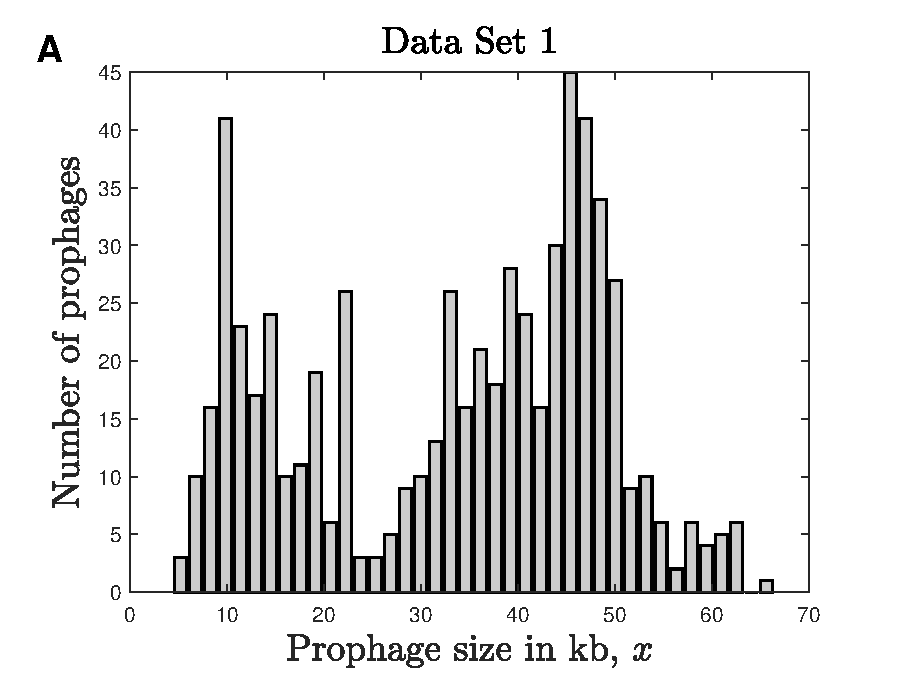
\includegraphics[scale=0.55]{bobbar}
    %\subcaption[subfigcapskip = 50pt]{Data Set 1.}
    %\label{fig:bob_bar}
    \end{subfigure}\hfill
    \begin{subfigure}[t]{0.45\textwidth}
    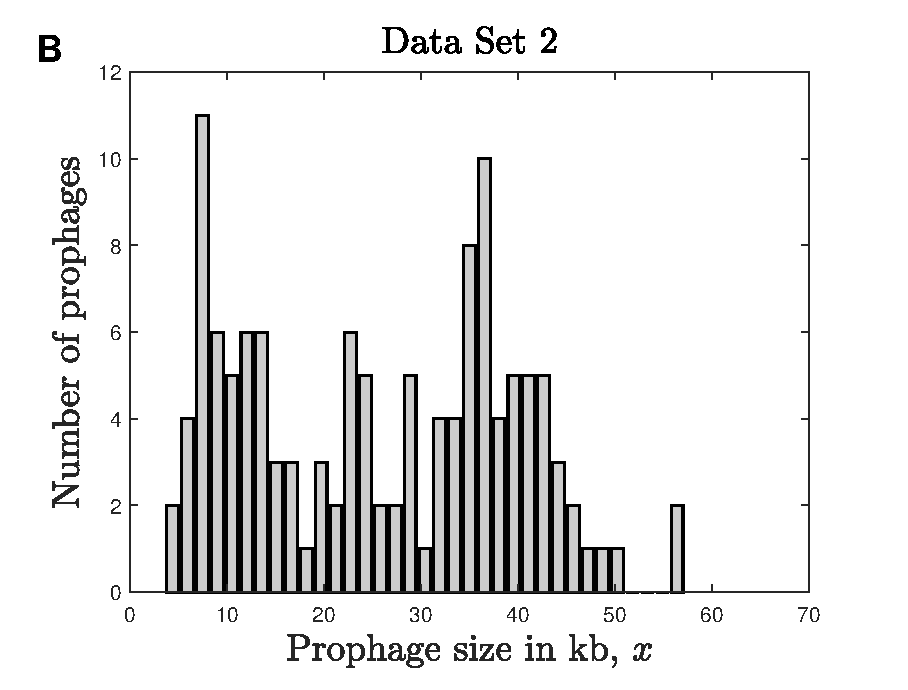
\includegraphics[scale=0.55]{desubar.eps}
       % \subcaption[subfigcapskip = 50pt]{Data Set 2. }
        %\label{fig:desu_bar}
    \end{subfigure}\hfill
    \begin{subfigure}[t]{0.45\textwidth}
    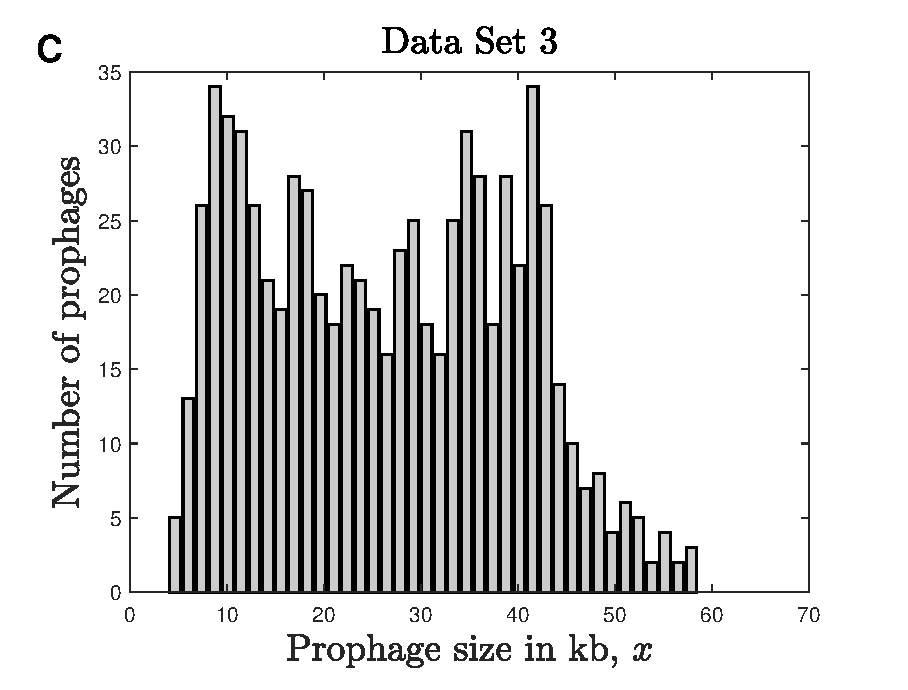
\includegraphics[scale=0.55]{ALCLbar.eps}
            %\subcaption[subfigcapskip = 50pt]{Data Set 3.}
            %\label{fig:ACL_bar}
    \end{subfigure}\hfill
     \begin{subfigure}[t]{0.45\textwidth} 
    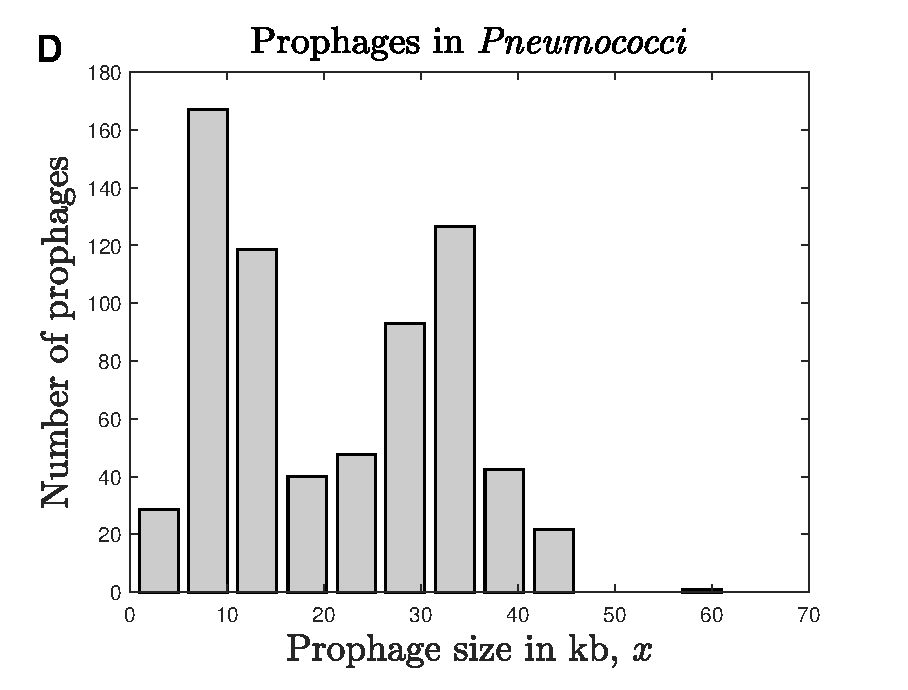
\includegraphics[scale=0.55]{brubar.eps}
    % \subcaption{Prophages in \textit{Pneumococci}.}
     %\label{fig:brug_bar}
     \end{subfigure}\hfill
    \caption[Prophage size distributions.]{ Prophage size distributions.   (A) Prophages identified in \textit{E.~coli} and \textit{S.~enterica} \citep{bobay_pervasive_2014}. (B) Prophages identified in \textit{Desulfovibrio} \citep{crispim_screening_2018}. (C) Prophages across a range of sequenced bacterial genomes \citep{leplae_aclame:_2010}.  (D) Prophages identified in \textit{Pneumococci} \citep{brueggemann_pneumococcal_2017}.}
\label{fig:data}
\end{figure}

%\renewcommand{\baselinestretch}{1.0}
\begin{table}[H]
\centering
\begin{tabular}{ p{1.2cm}p{1.5cm}p{1cm}p{1cm}p{1.5cm}p{3.5cm}p{3.5cm}}
\hline
Data Set & Prophage number & Min (kb)& Max (kb)& Average (kb)& Bacterial Species &Reference \\
\hline
1 & 624 &4.348& 66.345& 33.268 & \textit{E.~coli}, \textit{S.~enterica} &\cite{bobay_pervasive_2014}\\

2& 128 & 3.603 & 57.140 & 25.580 & \textit{Desulfovibrio} &\cite{crispim_screening_2018}\\

3& 737 & 3.918 & 58.560  & 26.450 & Diverse &\cite{leplae_aclame:_2010}\\
\hline
\end{tabular}
\caption{Summary of the three data sets analyzed in this study. }
\label{table:2}
\end{table}
%\renewcommand{\baselinestretch}{2.0}

\subsection{Our approach}
 The natural question that arises is: why are prophage size distriubutions so often bimodal?  In a preliminary investigation, \cite{bobay_pervasive_2014} arrived at the conclusion that the bimodal distribution in their data is neither due to taxonomic biases nor due to large neutral deletions of genetic material. 
 In addition, if there were substantial heterogeneity in the prophage integration rate over evolutionary time, we might expect greater diversity in the multimodal distributions observed across a range of bacterial species; in other words, it seems unlikely that the peak at shorter lengths in four datasets is due to a single historical ``burst" of prophage integration.
 The aim of our study is to investigate these prophage distributions in more detail and, using the available data, determine which evolutionary processes are necessary to explain these observations. 
 
 The organization of this article is as follows: in Section~\ref{mm}, we derive a partial differential equation that models the time evolution of the prophage distribution, including expressions for the effects of mutation, selection, horizontal gene transfer and induction. In Section~\ref{ns}, we describe our analysis of the model, including model selection and fitting the model to the available data sets. In Section~\ref{results}, we present the results of data fitting. Finally, in Section~\ref{discussion}, we discuss the conclusions derived from this analysis and suggest further directions.
  
\section{Model Derivation}\label{mm}
To better understand the observed distributions of prophage lengths, we seek an expression for the expected frequency of prophages of length $x$, $P(x)$, in a population of bacterial genomes.  Here $x$ is prophage length in kb, with $x_{0}<x<x_{M}$ ($x_{0}$ and $x_{M}$ are the minimum and maximum prophage length, respectively). We begin by considering the processes that change the distribution of prophages over time, and then solve for the expected steady state (long-term behavior) of the model. Let $Q(x,t)$ be the frequency of prophages of length $x$ at time $t$. After time step $\delta t$, this distribution may change due to: (1) new temperate viral genomes entering the bacterial genome; (2) horizontal gene transfer (HGT) adding new prophages or partial prophages to the existing prophage pool; (3) mutational degradation reducing prophage lengths; (4) selection promoting the proliferation of the bacterial population, and therefore the prophage population; and (5) induction removing prophages from the population . 

Taking into account these five possible processes,
we arrive at the following partial differential equation describing the time evolution of the prophage size distribution:
\begin{eqnarray}\label{pde}
\frac{\partial Q(x,t)}{\partial t}=\alpha f(x)+\, \beta \, g(x)\, +\frac{\partial}{\partial x}\left[D(x)Q(x,t)\right]+r_{S}\,S(x)\,Q(x,t)-r_{I}\,I(x)\,Q(x,t)\,\,.
\end{eqnarray}  
The five terms on the right describe the influx of new prophage via lysogeny, influx via HGT, mutational degradation, selection, and induction respectively.  
The distribution of interest, $P(x)$, if it exists, is the steady state solution of $Q(x,t),$ i.e., $P(x) = \lim_{t \rightarrow \infty}Q(x, t)$. 
In the following subsections we explain each of the terms in Equation \ref{pde} in greater detail, and derive mathematical expressions for the underlying functions. For this purpose, in subsection (\ref{genes}), we show that there is a linear relationship between the length of a prophage and the number of genes it contains.

\begin{table}[H]
\centering
\begin{tabular}{ p{2cm}p{12cm}}
\hline
%Function or parameter & Description \\
%\hline
$Q(x, t)$ & frequency of prophages of length $x$ (kb) at time $t$ \\
$P(x)$ & steady state solution of $Q(x,t)$\\
$f(x)$& length distribution of prophage sequences entering via lysogeny\\
$g(x)$ & length distribution of phages transferred by HGT\\
$D(x)$ &  mutational degradation rate\\
$S(x)$ & expected fraction of $r_S$ conferred by prophage of length $x$\\
$I(x)$ & probability that prophage carries genes required for induction\\

\hline
$\alpha$&  rate of lysogeny\\
$\beta$ & rate of horizontal gene transfer (HGT)\\
$r_{S}$ & selection coefficient (intact prophage)\\
$r_{I}$ & rate of induction\\
\hline
\end{tabular}
\caption{Model functions and parameters.}
\label{table:2M}
\end{table}

\subsection{Number of genes and length of prophage}\label{genes}

Genome size and number of genes are strongly correlated in prokaryotes \citep{gregory_synergy_2005}. 
 We used data available in the ACLAME database (\href{http://aclame.ulb.ac.be/}{http://aclame.ulb.ac.be}), to confirm that this relationship between sequence length and the number of genes extends to prophage sequences in bacterial genomes, as illustrated in Figure ~\ref{fig:genes}.   We find that the length of a prophage, $x$, and the number of genes it carries, $m$, are highly correlated (correlation coefficient $r = 0.912$).  We model this correspondence as the simple linear relation 
 $m = \kappa \,x$, with $x$ in kb and $\kappa = 0.808$ genes per kb, corresponding to 1.2 kb per gene.
 
\begin{figure}[H] 
\centering
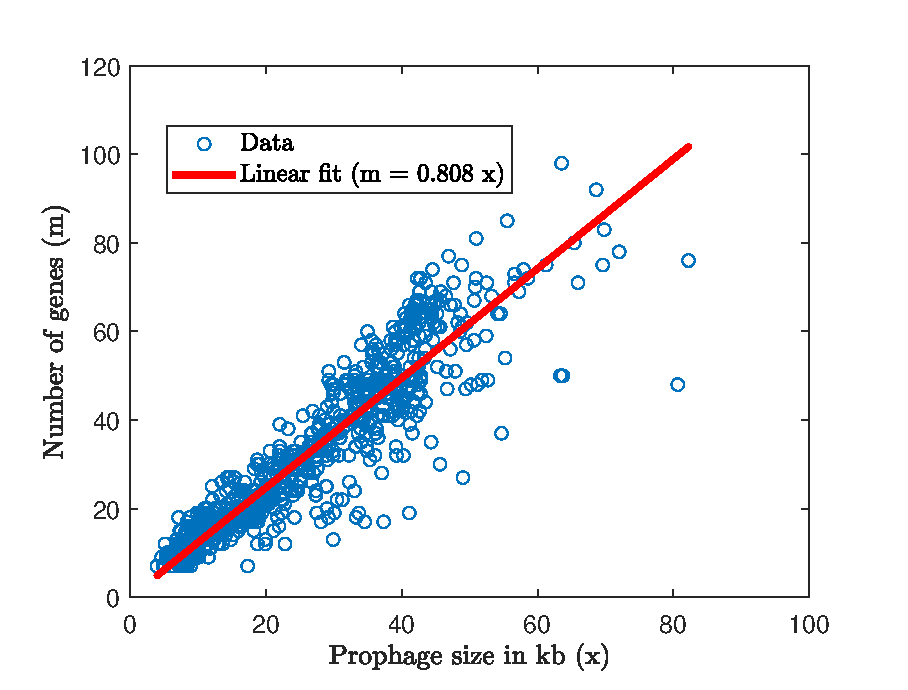
\includegraphics[scale=0.65]{genes}
\caption[Data showing the strong correlation between length of prophage and the number of genes on that prophage.]{Data from ACLAME database (\href{http://aclame.ulb.ac.be}{http://aclame.ulb.ac.be}), showing the strong correlation between length of prophage and the number of genes on that prophage.  All prophages in the database of length up to 85 kb were considered.}
\label{fig:genes}
\end{figure}

\subsection{Lysogeny}
The function $f(x)$ in Equation \ref{pde} represents the length distribution of prophages which enter bacterial genomes through lysogeny.  In other words, in the event that a phage genome will be integrated into a bacterial genome through lysogeny, $f(x)$ gives the probability density for the length of the phage genome to be integrated.  Thus, $f(x)$ captures not only the distribution of autonomous temperate phage genome lengths, but also any potential differences in lysogeny probabilities among these phages (see Appendix C for further details).

Most temperate phages are double-stranded (ds) DNA viruses \citep{szekely_single-stranded_2016}, although several single-stranded (ss) DNA phages have also been identified  as temperate \citep{krupovic_single-stranded_2015}.  We therefore expect that $f(x)$ might resemble the distribution of dsDNA phage lengths in nature.  Consistent with results reported for dsDNA phage (see Figure 1 in \cite{bobay_pervasive_2014}), we assume that the length distribution of these active phages may be multimodal, and that the minimum length for an autonomous phage is longer than the minimum length for a (possibly degraded and cryptic) prophage.  For convenience, we describe the multimodal distribution of active phages as the sum of $g =1$ to $3$ Gaussian probability density functions (i.e.\ a mixed distribution with up to three components):
\begin{eqnarray}\label{gs}
f(x) = \begin{cases} 
\sum_{i=1}^g {p_{i}e^{-\frac{(x-(\theta+\mu_{i}))^{2}}{\sigma_{i}^{2}}}} & x \geq \theta \\
0,  & x < \theta.
\end{cases}
\end{eqnarray}
where $p_{i} >0, \, \, \, \mu_{i} >0, \,\,\, \sigma_{i}>0$ for $i= 1$ to $g$ represent relative weights (in the convex combination), means and standard deviations of the component distributions, respectively. Note that $\theta$ in this expression gives the length of the smallest autonomous temperate phage. 
Temperate dsDNA phages have diverse genomes, with the smallest reported size of about $15$ kb (\textit{Bacillus phage Bam35c}) \citep{ravantti_comparative_2003, gaidelyte_linear_2005}; \cite{bobay_pervasive_2014} report that the smallest autonomous dsDNA phage that can infect enterobacteria is $30$ kb.  Here we assume that the smallest autonomous dsDNA phage that may successfully lysogenize a host has a genome size of $\theta = 20$ kb, however our results were not sensitive to this choice of threshold parameter (see Appendix B).

\subsection{Horizontal gene transfer (HGT)} 
HGT describes several processes by which genetic material is transferred from a donor bacterium to a recipient bacterium. The transfer of genetic material can be accomplished through \textit{conjugation}, \textit{transformation} and \textit{transduction}.  Although it has been inferred that transduction is 1000 times less likely than conjugation to transfer antibiotic resistance genes \citep{volkova_modeling_2014}, we note that transduction might be especially relevant to the HGT of chromosomal prophages.  In specialized transduction, a prophage erroneously excises from the bacterial genome, taking a neighboring piece of the host chromosome and possibly integrating an incomplete prophage sequence into the new bacterial host; in generalized transduction, DNA from elsewhere in the host chromosome (not necessarily adjacent to the prophage) is packaged into the viral capsid and transmitted to a new host \citep{touchon_embracing_2017}.  Since, for example, prophages can encode packaging-recognition sites (\textit{pac} signals) \citep{casjens_bacteriophages_2009}, transduction could play a significant role in the prophage size distribution. 

The function $g(x)$ in equation \ref{pde} represents the transfer of prophage sequences, or partial prophage sequences, into host genomes by any of these processes of HGT.  We reasoned that shorter DNA sequences should be transferred with higher probability than larger ones, therefore, we assume that $g(x)$ must be a non-negative decreasing function, i.e, $g(x) \geq 0$ and $g^{'}(x) \leq 0$ for all $x \in [0,x_M]$ (recalling that $x_M$ is the size of the largest prophage in the dataset).  The simplest function which satisfies these properties is a decreasing linear function, 
$g(x) = -x + x_M$.  The slope of this line is scaled by the free parameter $\beta$ representing the maximum rate of prophage integration via HGT.  We also investigated more complex functions describing HGT (data not shown) but these were not justified in data fitting. 

\subsection{Degradation} Mutational processes in bacterial genomes exhibit a strong bias toward deletion \citep{kuo_deletional_2009}, and mutational degradation may render intact prophages cryptic, i.e.\, incapable of induction or unable to form plaques.  Under the assumption that the probability of deletion is constant along the genome, we recover a linear relation between prophage sequence length and the rate of loss, $D(x) = r_{D}\,x,$ where again $x$ is the length of the prophage sequence in kb, and $r_{D}$ is the rate of degradation (kb of prophage sequence lost, per bacterial generation, per kb of prophage sequence).  Degradation from larger to smaller prophages depends on the gradient of the prophage length distribution, thus this process introduces an advective term.

\subsection{Selective advantage} \label{sel}
Integrated prophage often confer fitness benefits to their bacterial hosts \citep{bondy-denomy_when_2014}. Longer prophage sequences may encode a greater number of beneficial genes, conferring greater advantage to host cells and increasing the prophage population in turn. Let $n_b$ be the total number of potentially beneficial genes carried by phage. If $L$ is the number of genes in a prophage as it attaches to the bacterial genome, suppose after degradation $m$ intact genes remain. Then the probability, $\mathcal{P}(i),$ where $0< i \leq m,$ that the prophage of length $m$ carries  $i$ beneficial genes is 
\begin{eqnarray}
\mathcal{P}(i)= \frac{\binom{n_b}{i}\,\binom{L-n_b}{m-i}}{\binom{L}{m}}\nonumber,
\end{eqnarray}
which is a Hypergeometric distribution, with expected value $\sum_{i = 1}^{m}  i \,\mathcal{P}(i) = \frac{ n_b\,m}{L}$.  Converting this expectation to units of sequence length, a prophage degraded to length $x = m/\kappa$ from initial length $x_L = L/\kappa$ is expected to carry fraction $x/x_L$ of all possible beneficial genes (a result we will use in Equation \ref{sel1}). 


The probability that a prophage of length $x$ is a degraded version of an active phage of length $x_L$ is given by the proportion of active phages that have length $x_L$, as a fraction of all the active phages that might have given rise to this prophage:
\begin{eqnarray}\label{s1}
\mathcal{A}(x, x_L) = \begin{cases} 
0, & x > x_{L} \\
\dfrac{f(x_{L})}{\sum\limits_{y = \,x}^{x_{M}}f(y)},  & x \leq x_{L}.
\end{cases}
\end{eqnarray}
We assume that an active prophage confers an overall selective advantage $r_S$ per bacterial generation.  For mathematical tractability, we assume that the magnitude of this maximum selective effect does not vary with the initial length of the active phage sequence; this is a simplification that should be relaxed in future work.
We can then deduce $S(x)$, the expected fraction of $r_S$ that will be conferred by a prophage of length $x$, by conditioning and summing over all possible active phages that may have produced this prophage:
\begin{eqnarray}
\label{sel1}
S(x) = \sum\limits_{x_{L}=\,x}^{x_{M}} \mathcal{A}(x, x_{L})\frac{x}{x_{L}}.
\end{eqnarray}
Thus, the term $r_S S(x)$ gives the change in the intrinsic growth rate conferred on average by a prophage of length $x$.

Finally, we note that along with potential fitness benefits, prophage genes may also impose fitness costs on their hosts \citep{koonin_evolution_2009}.  The parameter $r_S$, which could be positive or negative, reflects the sum total of these costs and benefits.  Thus for example if the best-fit value of $r_S$ were negative, the model would predict that independent of induction, the carriage of prophage genes comes at a net cost to the host cell.

\subsection{Induction} \label{indu}
 Prophage may re-instigate the lytic life cycle, either spontaneously or in response to some stress, resulting in the death of the host cell and release of progeny phages.   As before, we let $L$ denote the number of genes in an active phage, while $m$ is the number of genes retained on a (possibly degraded) prophage.  Assume $n_l$ is the number of phage genes required for the loss of prophage from the bacterial genome through induction.  (Since the model tracks only the frequency of bacterial hosts carrying prophages of a given length, this loss could reflect either the excision of prophage from the bacterial genome, or the death of the bacterial host through lysis.)  The probability that a prophage carries the genes required for induction, given that after degradation it carries $m$ out of $L$ genes is:
\begin{eqnarray}
 \begin{cases} 
0, & m < n_l \\
\dfrac{\binom{L-n_l}{m-n_l}}{\binom{L}{m}},  & n_l \leq m \leq L.
\end{cases}\nonumber
\end{eqnarray}
We again use the parameter  $\kappa$ to convert between gene number and sequence length, and make use of  Stirling's approximation to simplify factorial terms.  We thus approximate the probability that a prophage, initially of length  $x_{L}$ but degraded to length $x$, contains the genes required for induction as:
\begin{eqnarray}
\mathcal{R}(x,x_L)\approx
 \begin{cases} 
0, & x < x_n \\
\dfrac{x^{\kappa \, x}\, (x_{L}-x_{n})^{\kappa (x_{L}-x_{n})}}{ x_{L}^{\kappa\, x_{L}}{(x- x_{n})}^{\kappa (x- x_{n})}},  &x_{n} < x \leq x_{L},
\end{cases}
\end{eqnarray}
where $x_n = n_l/\kappa$ is the length of the genes required.
The probability that a prophage of length $x$ is a degraded version of prophage of length $x_{L}$ is given by (\ref{s1}).
Thus, the overall probability that the prophage contains the genes required for induction (excision from the host genome), after conditioning and summing over all possible active phages that may have produced this prophage is given as:  
\begin{eqnarray}\label{ind}
I(x) \approx \sum \limits_{x_{L}=\,x}^{x_{M}}\mathcal{A}(x, x_{L})\,\mathcal{R}(x, x_{L}).
\end{eqnarray}
The parameter $r_I$ gives the induction rate, that is, the rate per prophage per bacterial generation at which prophages are lost from bacterial genomes due to induction.  Finally, we note that because prophages lost to induction may or may not contain the genes required for re-infection, we do not expect that the product $I(x) P(x)$ will directly yield the distribution of lysogenizing phages, $f(x)$ (but see Appendix C). 

Typical geometries of these five functions -- lysogeny, HGT, degradation, selection and induction -- are illustrated in Figure ~\ref{fig:func}.

\begin{figure}[htb!]
\captionsetup[subfigure]{labelformat=empty}
\begin{subfigure}[t]{0.5\textwidth}
\centering
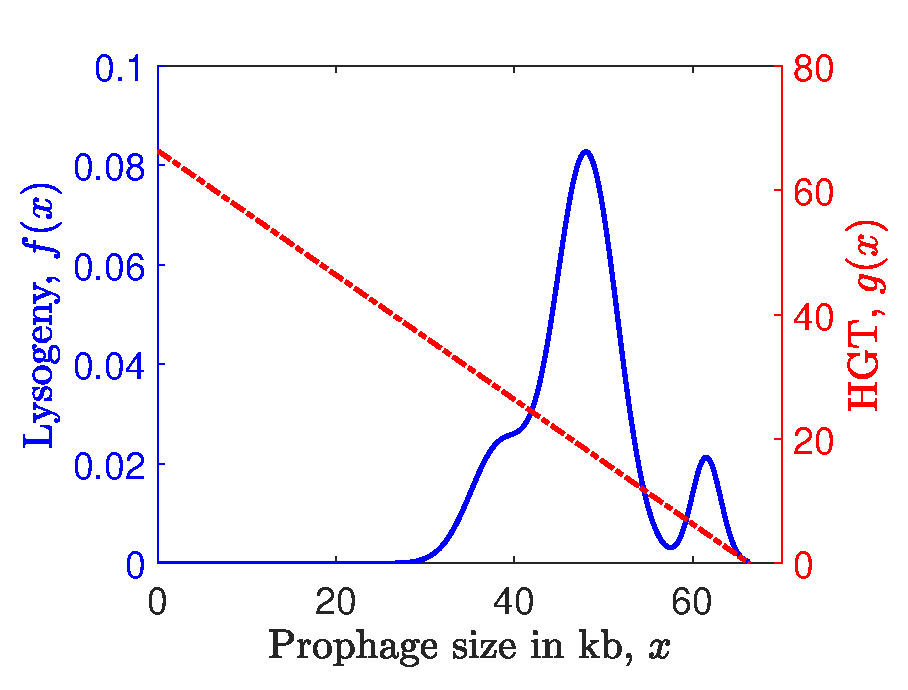
\includegraphics[scale=0.5]{phage1.eps}
\subcaption[subfigcapskip = 50pt]{}

\end{subfigure}\hfill
\begin{subfigure}[t]{0.5\textwidth}
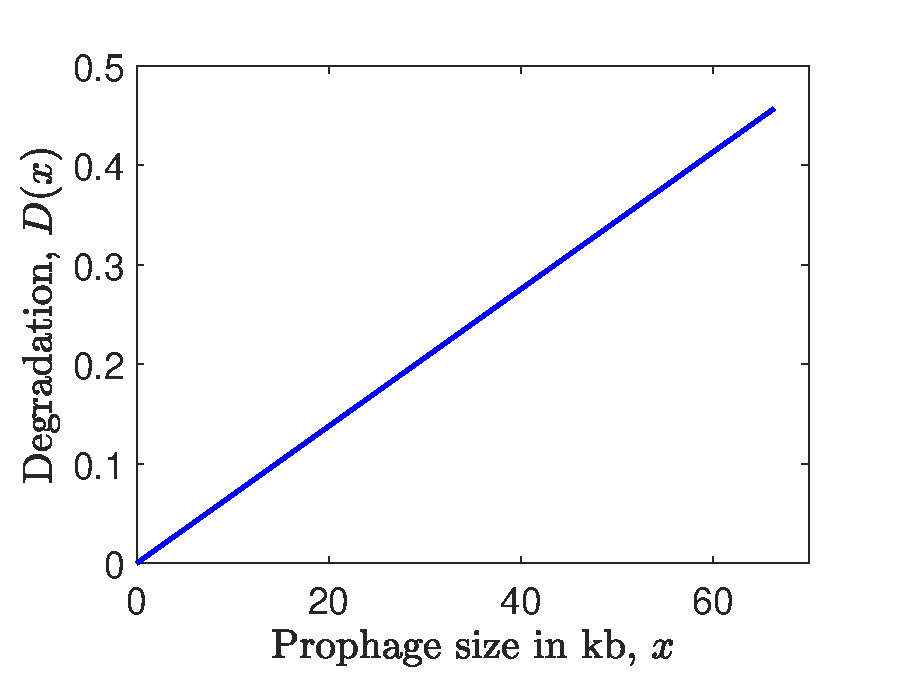
\includegraphics[scale=0.5]{deg2.eps}
            \subcaption[subfigcapskip = 50pt]{}
            
\end{subfigure} 
\begin{subfigure}[t]{0.5\textwidth}
\centering
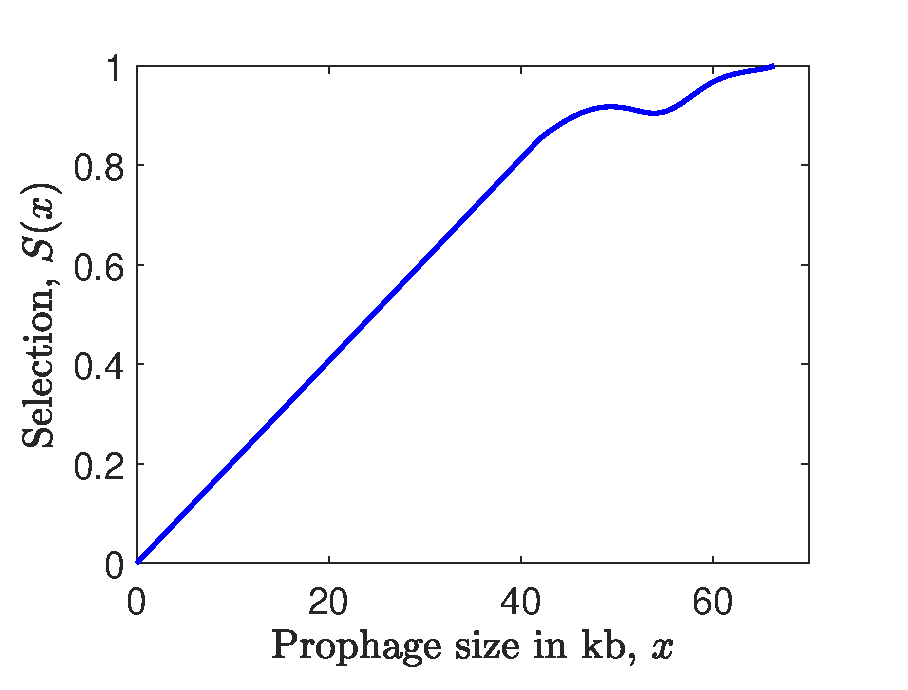
\includegraphics[scale=0.5]{sel3.eps}
\subcaption[subfigcapskip = 50pt]{}

\end{subfigure}
\begin{subfigure}[t]{0.5\textwidth}
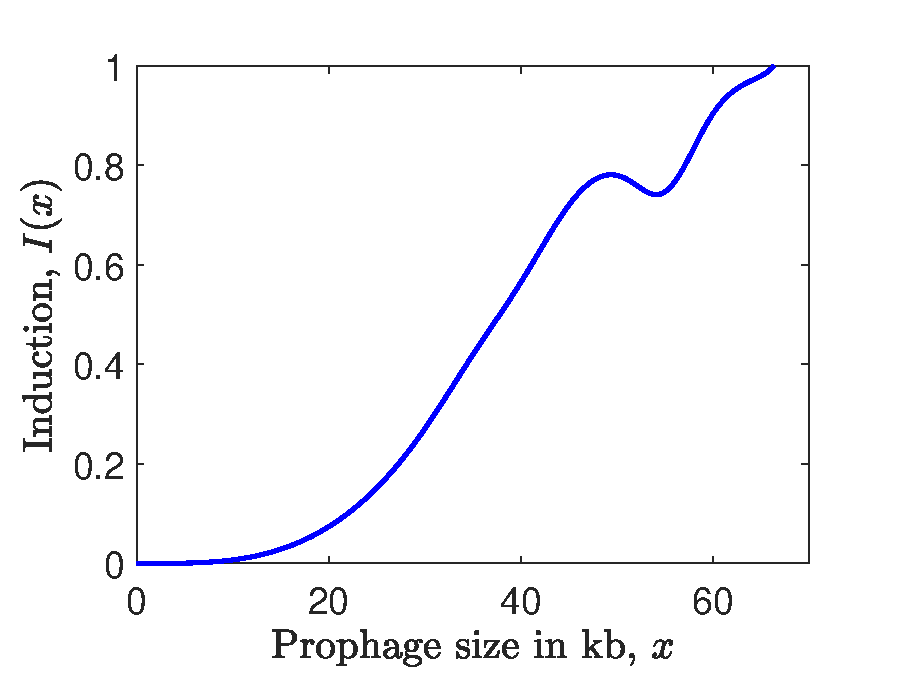
\includegraphics[scale=0.5]{ind4.eps}
\subcaption[subfigcapskip = 50pt]{}
\end{subfigure}
\caption[Example geometries of the influx distributions via lysogeny and HGT, as well as the degradation, selection and induction functions.]{Example geometries of the influx distributions via lysogeny and HGT (top panel, left and right axes respectively), as well as the degradation, selection and induction functions, plotted against prophage size. To illustrate the shapes of these functions, we have used parameters corresponding to the best fit to Data Set 1 (see Results to follow). Parameter values are $p_{1} = 17.95, \, \mu_{1} = 18.37, \, \sigma_{1} = 4.73,$ $p_{2} = 64.19, \, \mu_{2} = 28.06, \, \sigma_{2} = 4.93$, $p_{3} = 16.57, \, \mu_{3} = 41.54, \, \sigma_{3} = 2.32,$ $r_{D} = 0.0069$. }\label{fig:func}
\end{figure}
%%%%%%%%%%%%%%%%%%%%%%%%%%%%%%%%%%%%%%%%%%%%%%%%%%%%%%%%%%%%%%%%%%%%%%%%%%%%%%%%%%%%%%%%%%%
\subsection{Closed-form solution}

If we consider $\lim_{t \to \infty}\,Q(x, t)=P(x)$ and  $D(x) = r_{D}\,x$
then the differential equation generating the steady state solution of equation \ref{pde} is given by \begin{eqnarray}\label{appsol}
 \frac{d P(x) }{d x}+ \left(\frac{1}{x}+\mathcal{F}(x)\right)\,P(x)+\frac{\alpha}{r_{D}\, x} \, f(x)  + \frac{\beta}{r_{D}\,x} \, g(x) =0
\end{eqnarray}
where $\mathcal{F}(x) = (r_S\, S(x) - r_I\, I(x))/(r_D\,x)$.
Equation (\ref{appsol}) is first order linear ordinary differential equation and its solution is given by 
\begin{eqnarray}\label{ssol}
 P(x) &=&\frac{-\,e^{-\int{\mathcal{F}}(x)dx} }{r_D\, x}\,\int{(\alpha \,f(x)\, + \, \beta\, g(x))\,e^{\int{\mathcal{F}}(x)dx}dx}+\frac{C}{x}\, e^{-\int{\mathcal{F}}(x)dx},
\end{eqnarray}
where $C$ is a constant of integration.  Although in general a numerical approach is required to evaluate $P(x)$ due to the complexity of the functions $S(x)$, $I(x)$ and $f(x)$, the form of this solution will prove valuable in eliminating some solutions during model selection (see Table \ref{table:30} below).


\section{Model selection and data fitting}\label{ns}
Although lysogeny, HGT, degradation, selection and induction may all contribute to the maintenance of the prophage population in nature, we performed rigorous model selection to determine which of these processes are statistically justified in modeling the data.  This approach allows us to identify the key evolutionary processes underlying the prophage distribution, and to estimate the relative magnitude of their effects.

Since lysogeny is a necessary prerequisite for the prophage distribution, we considered  models that included incoming prophage ($f(x)$) but included or excluded HGT, degradation, induction and selection in all possible combinations.  Thus in total, we tested all $2^4 = 16$ possible models.  For brevity, Table \ref{table:30} lists the full model, as well as all possible models that exclude HGT; analogous models including HGT were also tested.  
\renewcommand{\baselinestretch}{1}

\begin{table}[htbp]
\centering
\begin{tabular}{ p{1cm}p{2cm}p{10.2cm}}
\hline
Model & Processes & Steady-state solution, $P(x)$\\
 & $f\,D\,I\,S \, g$  & \\
\hline
\\
1 & \checkmark \checkmark \checkmark \checkmark \checkmark& $\frac{-\,e^{-\int{\mathcal{F}}(x)dx} }{r_D\, x}\,\int{(\alpha \,f(x)\, + \, \beta\, g(x))\,e^{\int{\mathcal{F}}(x)dx}dx}+\frac{C}{x}\, e^{-\int{\mathcal{F}}(x)dx}$\\
\\
\hline
\\
2 & \checkmark \checkmark \checkmark \checkmark \ding{55}& $\frac{-\alpha \,\,e^{-\int{\mathcal{F}}(x)dx} }{r_D\, x}\,\int{f(x)\,e^{\int{\mathcal{F}}(x)dx}dx}+\frac{C}{x}\, e^{-\int{\mathcal{F}}(x)dx}$\\
\\
\hline
\\
3& \checkmark \ding{55} \checkmark \checkmark \ding{55}& $\frac{-\alpha f(x)}{S(x)-I(x)}$ where $S(x)\neq I(x)$\\
\\
\hline
\\
4& \checkmark  \checkmark \ding{55} \checkmark \ding{55}& \small{$-\frac{\alpha}{r_{D}}\frac{1}{x}e^{-\int \left(\frac{r_{S}}{r_{D}}\frac{S(x)}{x}\right)dx}\int f(x)e^{\int \left(\frac{r_{S}}{r_{D}}\frac{S(x)}{x}\right)dx}dx+\frac{C}{x}e^{-\int \left(\frac{r_{S}}{r_{D}}\frac{S(x)}{x}\right)dx}$}\\
\\
\hline
\\
5 & \checkmark  \checkmark \checkmark \ding{55} \ding{55} & $ -\frac{\alpha}{r_{D}}\frac{1}{x}e^{\int \left(\frac{r_{I}}{r_{D}}\frac{I(x)}{x}\right)dx}\int f(x)e^{-\int \left(\frac{r_{I}}{r_{D}}\frac{I(x)}{x}\right)dx}dx+\frac{C}{x}e^{\int \left(\frac{r_{I}}{r_{D}}\frac{I(x)}{x}\right)dx}$\\
\\
\hline
\\
6& \checkmark  \checkmark \ding{55} \ding{55} \ding{55}& $-\frac{\alpha}{r_{D}\,x}\int  f(x)dx+\frac{C}{x}.$\\
\\
\hline
\\
7& \checkmark  \ding{55} \checkmark \ding{55} \ding{55}& $\frac{\alpha f(x)}{I(x)},$ where $I(x)\neq 0.$\\
\\
\hline
\\
8 & \checkmark  \ding{55} \ding{55} \checkmark \ding{55}& $\frac{-\alpha f(x)}{S(x)},$ where $S(x) \neq 0.$\\
\\
\hline
\\
9 & \checkmark \ding{55} \ding{55} \ding{55} \ding{55}&
no steady-state solution\\
\\
\hline
\end{tabular}
\caption[A detailed description of the models considered.]{A detailed description of the models considered. Each model includes or excludes terms on the right-hand side of Equation \ref{pde} as indicated.  The analytical forms for the steady-state solutions, as shown in the right-most column, allow us to eliminate several models from further analysis (see text for details).
Here $\mathcal{F}(x) = \frac{r_S\, S(x)}{r_D\,x }- \frac{r_{I}\, I(x)}{r_D\, x}$ and $C$ is an arbitrary constant.}
\label{table:30}
\end{table}
%\end{landscape}

%\renewcommand{\baselinestretch}{2}

The first step in analyzing these models was to exclude models that are qualitatively unable to capture the prophage size distribution data. 
From the analytical solutions of models 3 (with both induction and selection present), 7 (with only induction present), and 8 (with only selection present), we see that in these cases, the steady-state solution $P(x)=0$ wherever the 
incoming phage distribution $f(x)=0$.  Thus these models predict the absence of prophage with lengths smaller than $\theta = 20$ kb.  These models are clearly unable to capture the distributions illustrated in Figure \ref{fig:data} and were excluded from further analysis.  This result makes intuitive sense: the three excluded models do not include degradation, and therefore cannot explain prophage with lengths shorter than the lengths of autonomous temperate phage.

We proceeded with model selection using the remaining five models (models 1, 2, 4, 5 and 6), fitted to each data set. For each model, we also allowed the function $f(x)$ (the incoming phage distribution) to be described by a mixed distribution incorporating one to three Gaussian distributions.  While the data sets included between $n$ = 128 and $n$ = 737 data points, the tested models included between $k$ = 4 and $k$ = 15 free parameters.  We used a finite difference scheme to obtain, numerically, the steady-state solution to the model, and compared this steady-state solution to the data, optimizing the log-likelihood to identify the best fit parameter values. The log-likelihood is defined as $\log(L) = \sum \log P(x_{i})$, 
where $x_{i}$ are the $n$ observed lengths of prophage sequences in the data set, $P(x)$ is the numerically obtained steady-state solution, and the sum is taken for $i = 1 \, \text{to} \, n$.
 To select the best model among the candidate models, we used the  Akaike Information Criterion (AIC) \citep{akaike_likelihood_1981}, defined as:
\begin{eqnarray}\label{aic}
\mbox{AIC} =2k -2\,\log\left(\hat{L}\right)
\end{eqnarray}
where $k$ is the number of free parameters, and $\log\left(\hat{L}\right)$ is the maximum log-likelihood. 

While the lowest AIC value corresponds to the best fit, it is possible that several candidate models may offer equivalently good fits; these correspond to models that cannot be rejected, statistically.  To address this issue, we compute the relative probability. If $AIC_{min}$ is the lowest $AIC$ value obtained for one of the candidate models, the relative probability \citep{burnham_model_2003} is defined for each candidate model as $R = \exp\left(\, ({AIC_{min}-AIC})/2\,\right)$.
The best fit model will thus have relative probability 1. If we imagine adding a single ``dummy" variable to the best fit model, that is, we add an additional parameter that has no effect on the fit, the AIC will increase by 2 and the log-likelihood will not change.  Thus the relative probability of the best fit model including an extra dummy parameter will be $\exp(-1) = 0.368$. We therefore reject candidate models with $R \leq \exp(-1)$.  If candidate models have relative probability values that exceed $\exp(-1)$, we are unable to reject them and consider them as possible ``best fits” to the data. 
%%%%%%%%%%%%%%%%%%%%%%%%%%%%%%%%%%%%%%%%%%%%%%%%%%%%%%%%%%%%%%%%%%%%%%%%%%%%

\section{Results}
\label{results}
We fit models 4, 5 and 6 to each of the three data sets, including in each model the possibility of up to three components in the incoming phage distribution, $f(x)$, and including or excluding HGT, $g(x)$.  
A full summary of the model-fitting results is provided in Appendix \ref{a2} (Table \ref{table:bob}, Table \ref{table:desu}, Table \ref{table:aclame} for Data Sets 1, 2 and 3, respectively).

Despite the reduced number of free parameters in the simpler models (an attribute rewarded by the AIC criterion), in no case did models 4 (degradation and selection), 5 (degradation and induction) or 6 (degradation) achieve the best fit to any of the data sets.  To illustrate, we have reproduced the fits obtained to Data Set 1 with these three models in Figure \ref{fig:noBi}.
\begin{figure}[H]
\centering
  \begin{subfigure}[t]{0.3\textwidth}
  \centering
 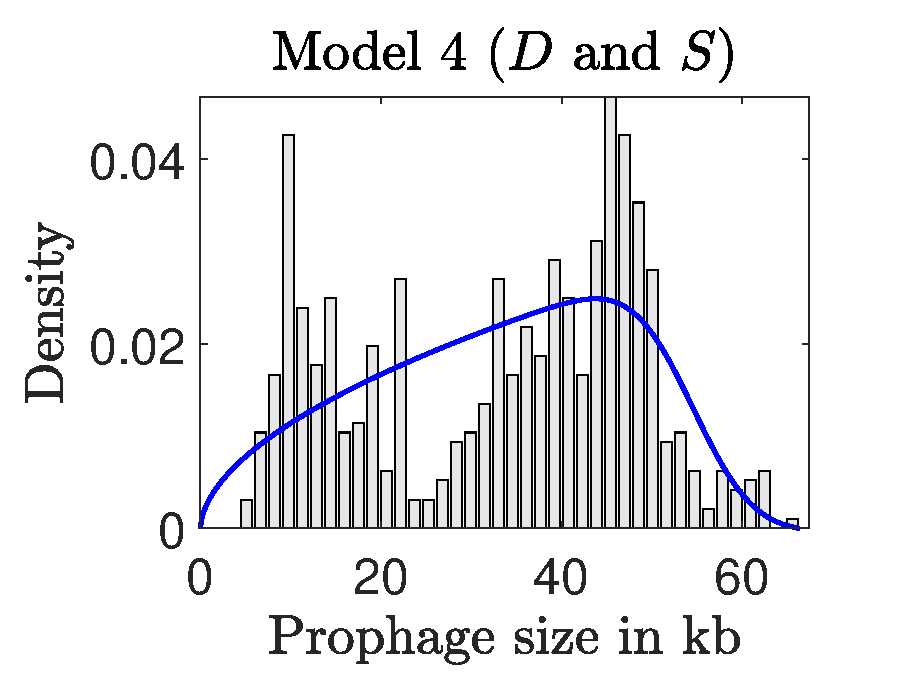
\includegraphics[scale=0.40]{DegSel.eps}
 %\subcaption[subfigcapskip = 50pt]{Model 4 ($D$ and $S$).}
% \label{fig:DegSel}
 \end{subfigure}\hfill
 \quad
 \begin{subfigure}[t]{0.3\textwidth}
 \centering
 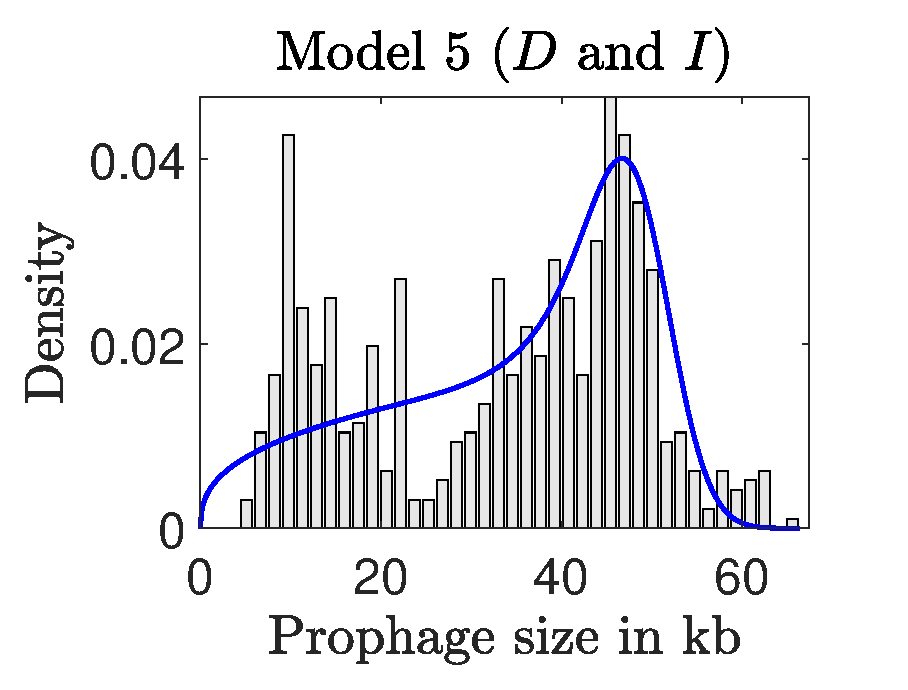
\includegraphics[scale=0.40]{DegInd.eps}
 %\subcaption[subfigcapskip = 50pt]{Model 5 ($D$ and $I$).}
 \label{fig:DegInd}
 \end{subfigure}\hfill
 \quad
 \begin{subfigure}[t]{0.3\textwidth}
  \centering
 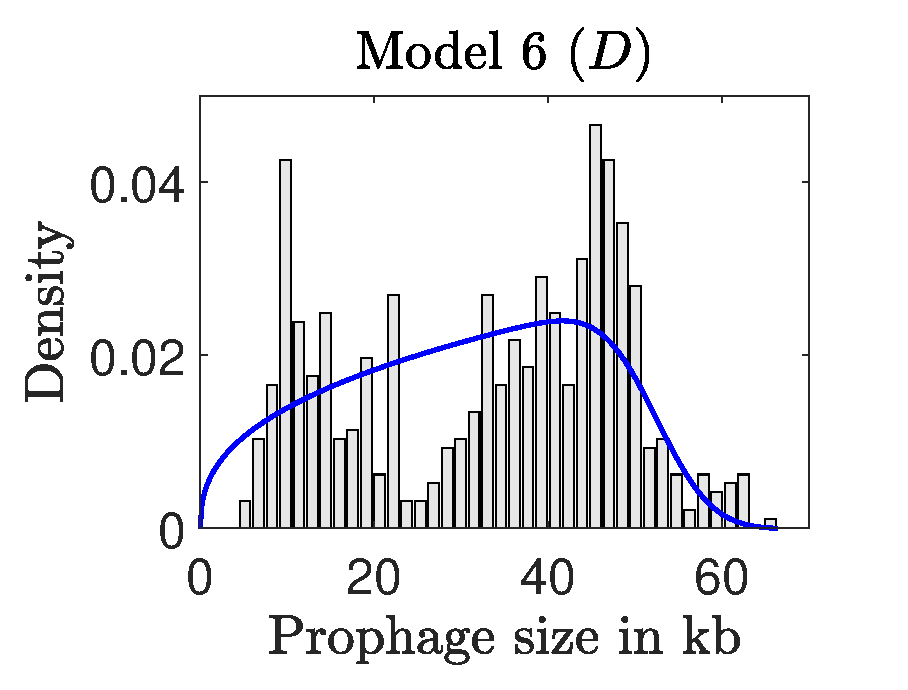
\includegraphics[scale=0.40]{onlyDeg.eps}
 %\subcaption[subfigcapskip = 50pt]{Model 6 ($D$).}
 \label{fig:Deg}
 \end{subfigure}
  \caption[Lines of best fit obtained to Data Set 1 by models 4, 5 and 6.]{ Lines of best fit ($P(x)$, shown in blue) obtained to Data Set 1 (histograms) by models 4, 5 and 6 (see Table \ref{table:30}); these models did not provide adequate fits to the data.}
\label{fig:noBi}
\end{figure}

 For all three data sets, then, model 2, as described by Equation \ref{pde} with $\beta =0$, provided the best fit, with varying degrees of complexity in the function describing the incoming phage distribution ($f(x)$).  We describe and illustrate these results below.

\subsection{Data Set 1}
 The best fit to these data from {\it E.~coli} and {\it S.~enterica} was obtained using the full model without HGT (model 2), with the distribution of incoming phages described by a mixture of three underlying Gaussian distributions ($g=3$).  This model has 14 free parameters (see Figure~5A). The second-best fit is the same model with HGT; this fit has relative probability 0.372 and thus cannot be rejected.  We note however that the contribution of HGT in this second-best fit is very small (see Table \ref{table:res}).  The best fits are illustrated in Figure~5B and 5C. Detailed results of data fitting are provided in
Table \ref{table:bob}, Appendix \ref{a2}.
%%%%%%%%%%%%%%%%%%%%%%%%%%%%%%%%%%%%%%%%%%%%%%%%%
\begin{figure}[H]
\begin{subfigure}[t]{0.3\textwidth}
\centering
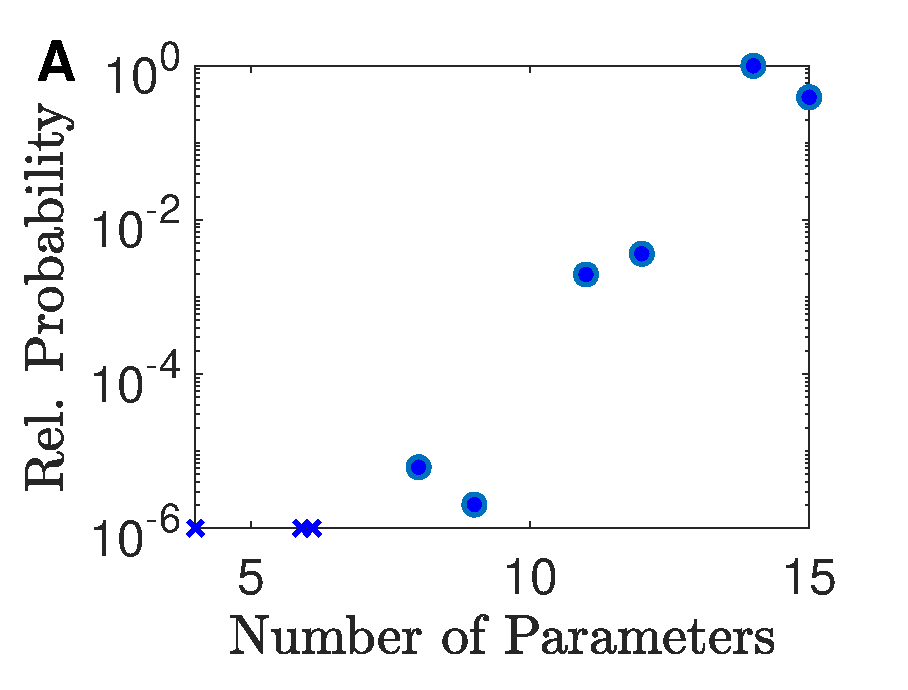
\includegraphics[scale=0.4]{bob_rel.eps}
%\subcaption[subfigcapskip = 50pt]
%\label{fig:bob_rel}
\end{subfigure}\hfill
\begin{subfigure}[t]{0.3\textwidth}
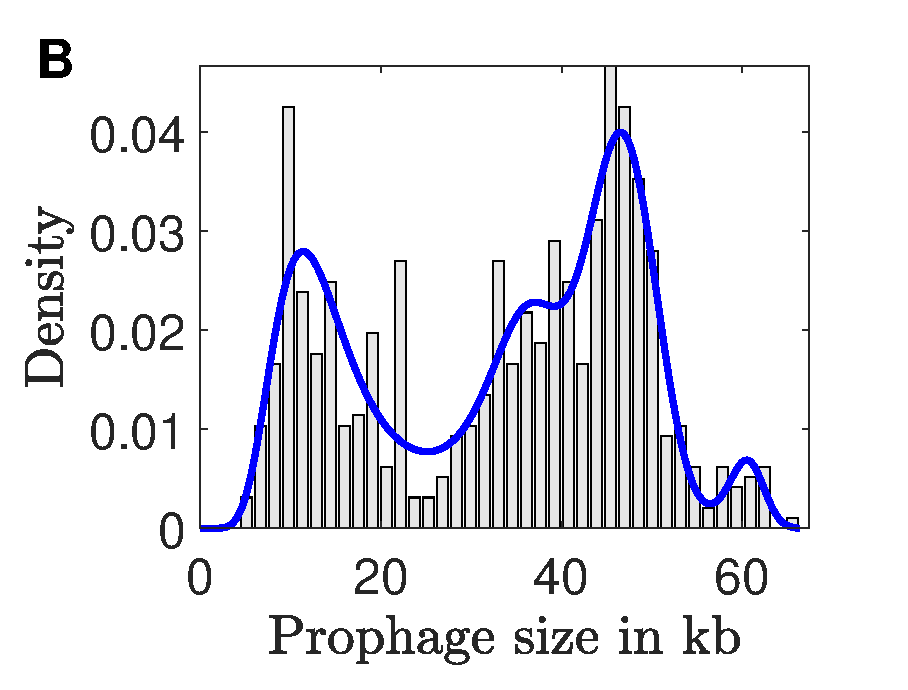
\includegraphics[scale=0.4]{bob_best_pdf.eps}
            %\subcaption[subfigcapskip = 50pt]{%Best fit.
%            }
            %\label{fig:bob_bestpdf}
\end{subfigure}\hfill
\begin{subfigure}[t]{0.3\textwidth}
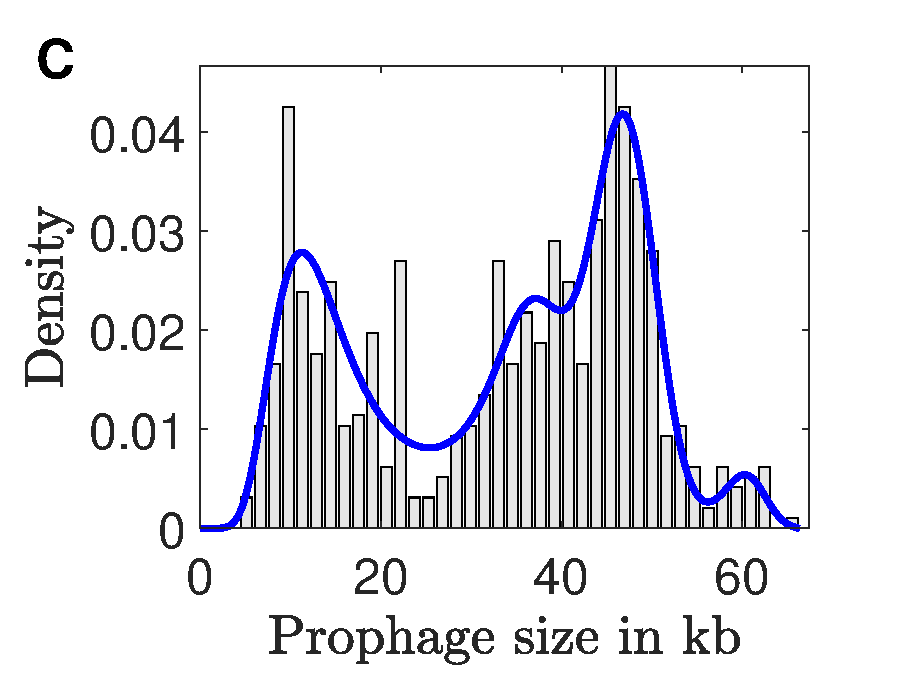
\includegraphics[scale=0.4]{bob_best2_pdf.eps}
%\subcaption[subfigcapskip = 50pt]
 %\label{fig:bob_best2_pdf}
 \end{subfigure}\hfill
\caption[Model fitting results for Data Set 1.]{ Model fitting results for Data Set 1.  (A) The relative probability of candidate models for Data Set 1, plotted as a function of the number of parameters in that model; crosses indicate relative probabilities $\leq 10^{-6}$. (B) The best fit predicted by the model ($P(x)$, blue curve) to Data Set 1 (histogram). The best fit included 14 free parameters. (C) The second-best fit  model (blue curve) to Data Set 1 (histogram). The second-best fit included 15 free parameters.}
\end{figure}
%%%%%%%%%%%%%%%%%%%%%%%%%%%%%%%%%%%%%%%%%%%%%%%%%%%%%%%%%%%%%%%%%%%%%%%%%%%%%%%%%%%%%%%%%%%%%%%%%%%%%%%%%%%%%%%%%%%%
\subsection{Data Set 2} 
The prophage length distribution from {\it Desulfovibrio} was best described by the full model without HGT, and a single Gaussian describing the incoming phage lengths ($g=1$, 8 parameter model), see Figure~6A.
This fit is illustrated in Figure~6B. Details are provided in Table \ref{table:desu} in Appendix \ref{a2}. 
%%%%%%%%%
\begin{figure}[H]
 \begin{subfigure}[t]{0.5\textwidth}
\centering
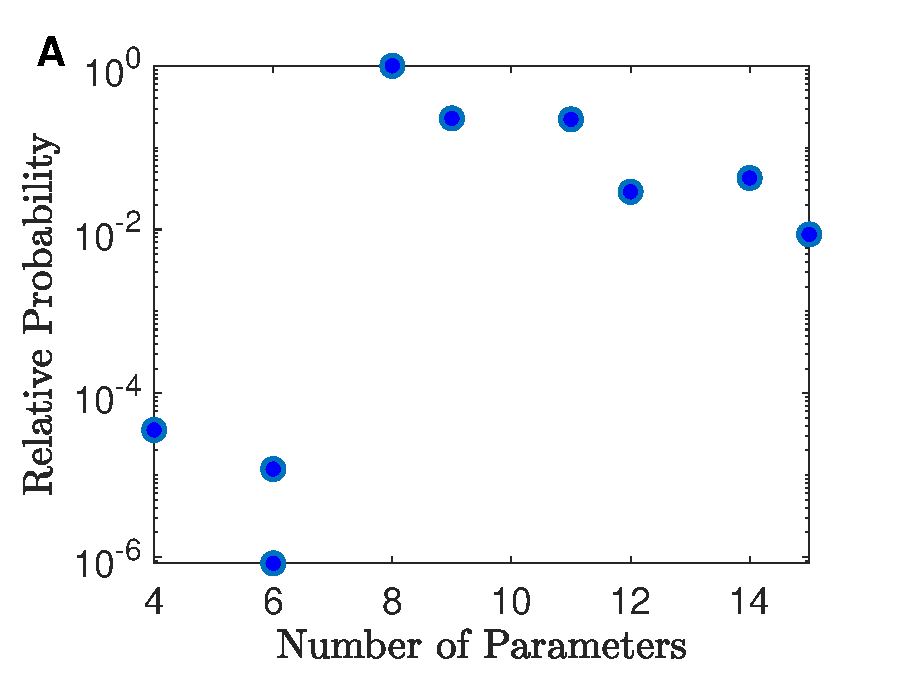
\includegraphics[scale=0.5]{desu_rel.eps}
%\subcaption[subfigcapskip = 50pt]{}
%\label{fig:desu_rel}
\end{subfigure}\hfill
\begin{subfigure}[t]{0.5\textwidth}
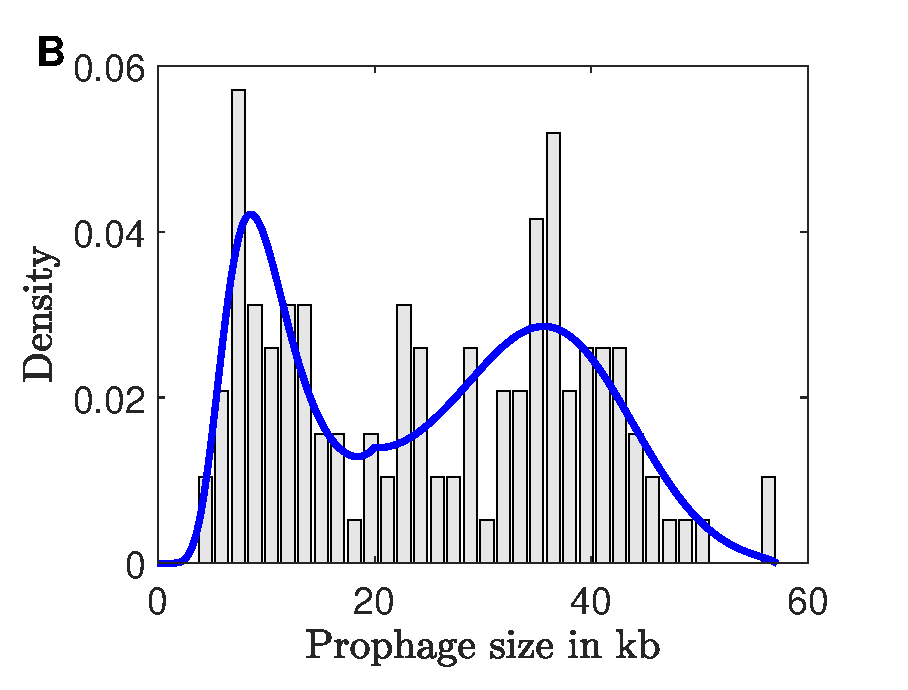
\includegraphics[scale=0.5]{desu_best_pdf.eps}
            %\subcaption[subfigcapskip = 50pt]{}
            %\label{fig:desu_bestpdf}
\end{subfigure}\hfill
\caption[Model fitting results for Data Set 2.]{ Model fitting results for Data Set 2. (A) The relative probability of candidate models for Data Set 2, plotted as a function of the number of parameters in that model.  (B) The best fit predicted by the model ($P(x)$, blue curve), to Data Set 2 (histogram). The best model includes 8 free parameters and has relative probability 1. 
}
\end{figure}
%%%%%%%%%%%%%%%%%%%%%%%%%%%%%%%%%%%%%%%%%%%%%%%%%%%%%%%%%%%%%%%%%%%%%%%%%%%%%%%%%%%%%%%%%%%%%%%%%%%%%%%%%%%%%%%%%%
\subsection{Data Set 3} 
The prophage length distribution from the ACLAME database was also best described by the full model with a single Gaussian describing incoming phage ($g=1$, 8 parameter model), see Figure~7A.
The best fit is illustrated in
Figure~7B.
Model fitting details are provided in Table \ref{table:aclame} in Appendix \ref{a2}. 
%%%%%%%%%%%%%%%
\begin{figure}[H]
 \begin{subfigure}[t]{0.5\textwidth}
\centering
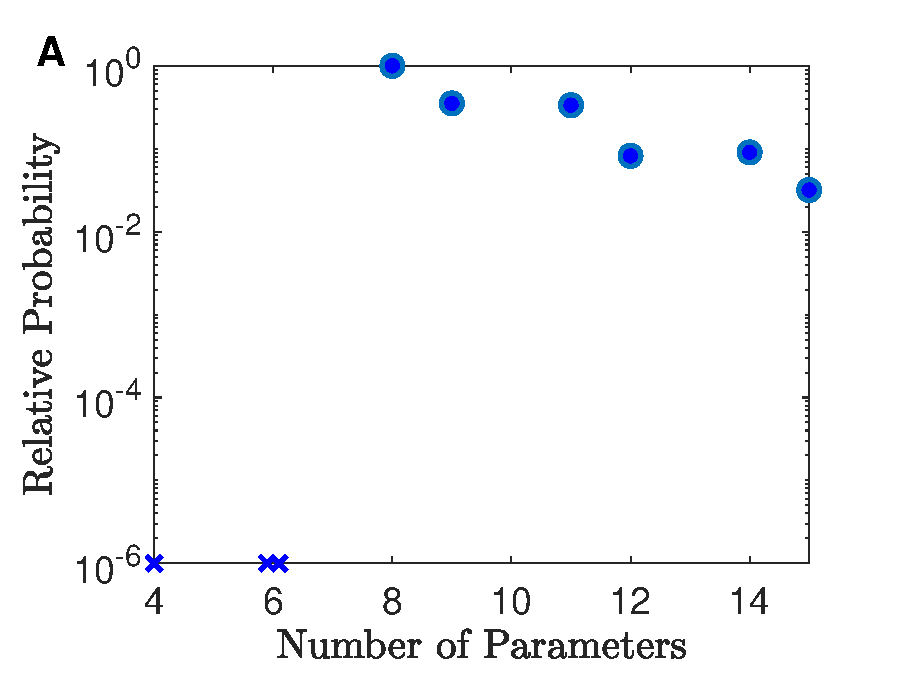
\includegraphics[scale=0.5]{aclame_rel.eps}
%\subcaption[subfigcapskip = 50pt]{}
%\label{fig:aclame_rel}
\end{subfigure}\hfill
\begin{subfigure}[t]{0.5\textwidth}
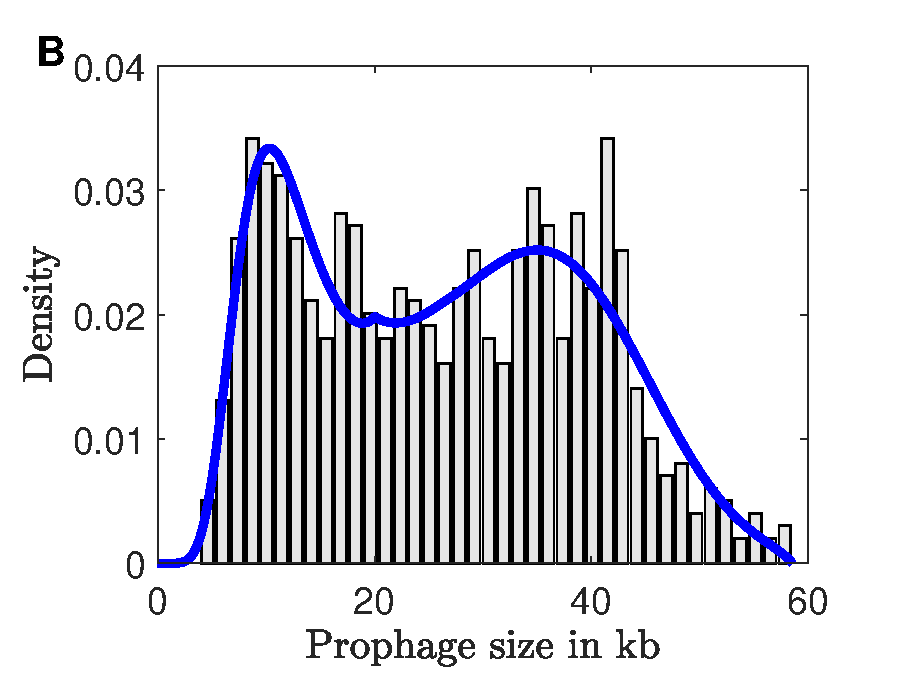
\includegraphics[scale=0.5]{aclame_best_pdf.eps}
            %\subcaption[subfigcapskip = 50pt]{}
            %\label{fig:aclame_bestpdf}
\end{subfigure}\hfill
\caption[Model fitting results for Data Set 3.]{ Model fitting results for Data Set 3. (A) The relative probability of candidate models for Data Set 3, plotted as a function of the number of parameters in that model; crosses indicate relative probabilities $\leq 10^{-6}$.
 (B) The best fit predicted by the model ($P(x)$, blue curve), to Data Set 3 (histogram). The best model includes 8 free parameters and has relative probability 1. 
}
\end{figure}

Table \ref{table:res} provides a summary of the best-fit parameter values obtained for the three data sets.  A sensitivity analysis, using Data Set 1, indicates a high degree of confidence in the parameter values, that is, all parameters are well-constrained by the data (see Appendix B).  However some care must be taken in interpreting these numerical values.  We present these rates in comparable units and address the implications of the quantitative results further in the Discussion.

%\renewcommand{\baselinestretch}{1}

% Table generated by Excel2LaTeX from sheet 'Sheet1'
%\begin{landscape}
\begin{table}[htbp]
%\renewcommand{\baselinestretch}{1}
  \centering
   \begin{tabular}{ p{0.5cm}>{\raggedright\arraybackslash}p{4.2cm}p{1.4cm}p{1.4cm}p{1.4cm}p{1.4cm}p{1.4cm}p{1.4cm}}
 \hline
 & & \multicolumn{2}{c}{Data Set 1}& \multicolumn{1}{c}{Data Set 2}& \multicolumn{1}{c}{Data Set 3} & \\
\multicolumn{2}{c}{\bf Parameter}  & best & 2\textsuperscript{nd} best &  &  & \multicolumn{1}{c}{\bf Mean$^\dag$}\\
 \hline
 $\alpha $   & Relative rate of lysogeny   & 0.1301  & 0.1982 & 0.1191 & 0.0734 & 0.1175\\
 \\
  $r_D$   & Relative rate of degradation   &0.0069  &0.01361& 0.0051 & 0.0052 & 0.0066\\
 \\
 $r_S$ &   Relative selection coeff. (intact prophage) &0.3137  & 0.7276 & 0.2397 & 0.2249 & 0.3110 \\
 \\
 $r_I$    & Relative rate of induction &0.6169 & 1.1139 & 0.5291 & 0.4713 & 0.6025\\
 \\
 $n_l$ &  Number of genes required for induction
 &2.440  &1.9512 & 2.440  & 2.5856  & 2.4198 \\
 \\
 $\beta$ & Relative rate of horizontal gene transfer & ----& $8.76 \times 10^{-13}$  & ---- & ---- & $8.76 \times 10^{-13}$\\ 
  \hline
\end{tabular}
    \caption[Parameter values for the best fits.]{Parameter values for the best fits. $^\dag$Mean across all data sets, weighted by relative probability for Data Set 1.}
    \label{table:res}%
\end{table}%
%\renewcommand{\baselinestretch}{2.0}

\section{Discussion}
\label{discussion}

Because we can only fit the steady-state solution of Equation \ref{pde} to the data, the resulting rates are only meaningful relative to other rates in the model.
Thus, although the time units of the best-fit rates are an arbitrary number of generations, we can express each of these rates relative to the induction rate.  This allows us to compare the evolutionary forces at play in terms of what we will call the ``expected prophage lifetime", that is, the average time between lysogeny and induction, for prophages that retain all the genes necessary for induction.  We find that the time between lysogeny events (new prophages entering the genome) is about 5 prophage lifetimes, while the selection coefficient, for an intact prophage, is approximately 0.5 per prophage lifetime.  If a prophage remains in the host genome for 100 bacterial generations before induction, for example, this selection coefficient would correspond to a selection coefficient $s=0.004$ per bacterial generation.  Finally, we predict that degradation of the prophage genome occurs at a rate of about 0.01 kb per kb in the prophage genome, per prophage lifetime.  Thus on average the model predicts that prophages have lost only 1\% of their genome to degradation at the time of induction.  These normalized rates are presented in summary in Table \ref{tab:rates}.

%\renewcommand{\baselinestretch}{1.0}

\begin{table}[H]
%\renewcommand{\baselinestretch}{1.0}
\centering
    \begin{tabular}{l r}
\hline
    \multicolumn{2}{c}{{ Rates expressed per expected prophage lifetime}}\\
    \hline
    {\bf Lysogeny} & 0.20\\
rate at which new prophage enters genome &  \\ 
{\bf Degradation}  & 0.01 \\
kb lost per kb of prophage genome &  \\
{\bf Selection} & 0.52 \\
overall selection coefficient per prophage lifetime & \\
{\bf Induction} & 1.00 \\
rate at which fully competent prophage induces & \\
\hline
    \end{tabular}
    \caption[Rates of the processes in the model, normalized by the induction rate. ]{Rates of the processes in the model, normalized by the induction rate.  Induction rate and selection coefficient are provided for fully intact (non-degraded) phage.  See text for details.}
    \label{tab:rates}
\end{table}

%\renewcommand{\baselinestretch}{2.0}


From these normalized rates, a picture emerges in which induction is the dominant fate for active prophages, occurring at a much higher rate than any other process.  New prophages enter the bacterial genome, on average, at a rate that is about one fifth of the induction rate.  These new sequences degrade very slowly relative to their induction rate, an observation that seems reasonable given that prophages would be unable to induce if degradation were rapid.   Despite the slow degradation rate, over evolutionary time smaller and smaller prophages accrue in host genomes.  These are maintained due to the balance between two effects: induction and selection.  In particular, short prophage sequences typically lack the genes required for excision or induction, but may still confer some benefit to their host.

Thus, our model predicts that the peak on the right of the prophage size distribution is due to the contribution of autonomous free phage, entering bacterial genomes via lysogeny, the term $\alpha f(x)$ in our model.  In contrast, the peak on the left is maintained in the region for which $r_s S(x) > r_I I(x)$, that is, where the benefits of selection outweigh the costs of induction, as illustrated in Figure ~\ref{fig:combine}.

\begin{figure}[H]
\centering
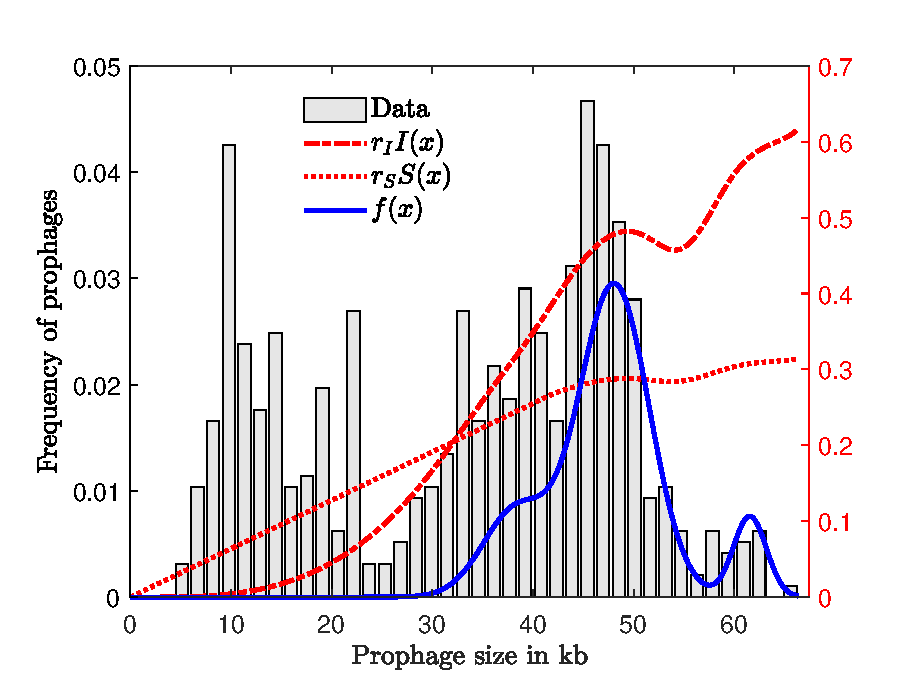
\includegraphics[scale=0.65]{combined1}
\caption[Components of the best-fit model prediction for Data Set 1.]{Components of the best-fit model prediction for Data Set 1 (histogram, left axis).  The distribution of autonomous temperate phages ($f(x)$, solid curve) is plotted along with the induction curve ($r_I I(x)$, dash-dotted, right axis) and the selection curve ($r_{S}S(x)$, dotted, right axis); induction and selection intersect near 30 kb.}
\label{fig:combine}
\end{figure}

An unexpected result of our analysis is that a process that preferentially adds prophages of shorter lengths to bacterial genomes (the process we describe as HGT in the model derivation) was not required to provide a fit to any of the three data sets.  For Data Set 1, HGT was included in the second-best fit, but the overall rate of HGT was extremely small relative to other rates in the model.  These results of course do not preclude a role for HGT in the maintenance of prophages in bacterial genomes, but indicate that HGT is not required to explain the empirical data currently available.  As mentioned previously, it seems likely that transduction may be the most important HGT process for prophages, and transduction rates are inferred to be low relative to other modes of HGT \citep{volkova_modeling_2014}.

Our findings suggest that a minimum of two to three prophage genes are required to enable prophage excision from the bacterial chromosome. The excision of phage $\lambda$, for example, requires at least two enzymes, an integrase and  exonuclease, which are produced from a single transcript encoding the $xis$ and $nit$ genes \citep{weitz_quantitative_2017}. We would of course expect wide variability in these steps across phage-host systems.  For example, phage Mu replicates first and then excises from the host chromosome \citep{10.2307/66893}, and would presumably require further intact genes for excision.

The relation between prophage and their bacterial hosts may either be parasitic or mutualistic depending on the balance between the cost the bacterial host incurs due to the integration of foreign DNA into its genome, and benefits conferred by the foreign DNA to the bacterial host \citep{shapiro_evolution_2018}. The biggest cost is incurred by induction, although due to the compactness of bacterial genomes, small insertions of foreign DNA may result in significant energy costs as well \citep{koonin_evolution_2009}.  Our results predict a tipping point between parasitism and mutualism, the point at which $r_I I(x) = r_S S(x)$.  Shorter prophage sequences are unlikely to maintain all the genes required for induction, and our model predicts that they persist at high frequencies in host genomes because of the selective benefits they still confer.  Thus the peak on the left of the bimodal prophage distributions may correspond to predominantly mutualistic prophage, consistent with high levels of purifying selection inferred for prophage genes using comparative genomics \citep{bobay_pervasive_2014}.  Metagenomic data, that is, prophage distributions obtained from environmental samples of bacterial populations, could help clarify the role of positive selection in maintaining prophage sequences.

Although an active body of research addresses the comparison and refinement of algorithms for prophage identification \citep{song_prophage_2019, sousa_phageweb_2018}, short prophage remnants can be difficult to detect and are likely underrepresented in the available data.  For example, prophage remnants with sequence similarity to short mobile genetic elements were excluded from Data Set 1 \citep{bobay_pervasive_2014}, and a minimum of six phage-like genes are required to identify phage gene clusters in the PHAST search tool \citep{zhou_phast:_2011}. 
Most algorithms to date rely on homology-based techniques to identify prophages, making it difficult to detect prophages that are not similar to known phages (but see \cite{akhter_phispy:_2012}), and making the identification of shorter sequences more challenging.   
This detection bias likely shifts the position of the lower peak in bimodal prophage distributions -- the true peak in the data might occur at even shorter prophage lengths -- but would not affect our conclusions regarding the underlying mechanisms in play.

We note that for one of the three data sets in this analysis, the best fit to the data was obtained using 14 of 15 possible parameters, that is, the best fit supported a relatively complex model.  This implies that as richer data sets become available, further features could, and should, be added to the model to better describe the prophage distribution.  As mentioned previously, two assumptions that could clearly be relaxed are that all phage genomes, irrespective of their length, offer the same average selective benefit to their host, and require the same number of genes for induction.  In reality, longer active phages presumably have the capacity to encode further beneficial functions and more complex excision mechanisms.  Another assumption, inherent in our approach, is that degraded prophage have lost the genes required for induction, or the genes conferring benefit to the host, in proportion to their total gene loss.  Thus the selection or induction rates depend only on prophage length. A more nuanced (but less tractable) approach will be to follow the loss and enrichment of specific classes of genes in degraded prophage sequences.

\section*{Acknowledgements}
The authors are indebted to Alita Burmeister for several insightful comments that strengthened the work.  The Natural Sciences and Engineering Research Council of Canada is gratefully acknowledged for funding.
 
\addcontentsline{toc}{chapter}{Bibliography}
\bibliographystyle{abbrv}
\bibliography{refrence}
% \begin{appendices}
% \chapter{Results from model selection and data fitting}\label{a2}
% The AIC value is the measure of loss of information for the model under consideration and is an ordinal number, used for ranking models. The lowest AIC value corresponds to the best fit.  If the number of data points are small enough compared to the number of parameters then the AIC value is not penalized enough. To remedy this problem a second order Akaike Information criteria, the corrected Akaike Information Criteria (AICc), is defined. The corrected  Akaike Information Criteria (AICc) is given as \citep{burnham_model_2003}:
% \begin{eqnarray}\label{aicc}
% AIC_c=AIC + \frac{2k(k+1)}{n-(k+1)}.
% \end{eqnarray}
% As the number of data points becomes large enough, AICc values converge to AIC values and either of these criteria can be used to determine the best fit model amongst the candidate models \citep{burnham_model_2003}. In the tables to follow, we provide both AIC and AICc values, and compute relative probabilities using the AICc values.
%   \section{Data Set 1}
% \begin{table}[H]
% \centering
% \begin{tabular}{ p{1cm}p{2cm}p{2cm}p{2cm}p{2cm}p{3cm}  }
% \hline
% \# & Parameters & AIC & AICc& Log-likelihood & Relative probability (AICc) \\
% \hline
% 1&                        15&          4884.1734&          4884.9642&         -2427.0867&         0.3719\\
% 2&                        14&          4882.2952&          4882.9860&         -2427.1476&         1\\
% 3&                        12&          4893.5207&          4894.0322&         -2434.7603&       0.0039\\
% 4&                        11&          4894.7613&          4895.1920&         -2436.3807&       0.0022\\
% 5&                         9&          4908.5087&          4908.8014&         -2445.2544&      2.4788e-06\\
% 6&                         8&          4906.2759&          4906.5097&         -2445.1379&      7.7964e-06\\
% 7&                         6&          5044.8136&          5044.9499&         -2515.9068&      6.7604e-36\\
% 8&                         6&          5069.6683&          5069.8042&         -2528.8341&      2.7098e-41\\
% 9&                         4&          5063.9143&          5063.9788&         -2527.9571&      4.9878e-40\\
% \hline
% \end{tabular}
% \caption[Number of parameters, AIC, AICc values, log-likelihood and the corresponding relative probabilities for Data Set 1.]{Number of parameters, AIC, AICc values, log-likelihood and the corresponding relative probabilities for Data Set 1 \citep{bobay_pervasive_2014}. The best fit model includes a mixed distribution to describe autonomous temperate phages ($g$=3), degradation, induction and selection. The second best fit model is the same model with HGT and has relative probability $0.3791$.}
% \label{table:bob}
% \end{table}
% \section{Data Set 2}
% \begin{table}[H]
% \centering
% \begin{tabular}{ p{1cm}p{2cm}p{2cm}p{2cm}p{2cm}p{2cm}  }
% \hline
% \# & Number of Parameters & AIC & AICc& Log-likelihood  & Relative probability \\
% \hline
% 1&                         15&          993.726&          998.583&         -480.863&       0.0016\\
% 2&                        14&          990.549&          994.797&         -480.275&        0.0108\\
% 3&                        12&          991.327&          994.492&         -482.663&         0.0126\\
% 4&                        11&           987.247&          989.937&         -481.624&         0.123\\
% 5&                         9&          987.197&          989.062&          -483.599&         0.191\\
% 6&                         8&          984.237&          985.749&         -483.119&          1\\
% 7&                         6&          1006.929&          1007.855&         -496.464&      1.585e-05\\
% 8&                         6&          1012.234&          1013.159&         -499.117&       1.117e-06\\
% 9&                         4&          1004.729&          1005.216&         -497.364&      5.927e-05\\
% \hline
% \end{tabular}
% \caption[Number of parameters, AIC, AICc values and the corresponding relative probabilities for Data Set 2.]{Number of parameters, AIC, AICc values and the corresponding relative probabilities for Data Set 2 \citep{crispim_screening_2018}. The best fit model includes degradation, induction and selection as well as one Gaussian distribution to describe autonomous temperate phages ($g$=1).}
% \label{table:desu}
% \end{table}
% \section{Data Set 3}
% \begin{table}[H]
% \centering
% \begin{tabular}{ p{1cm}p{2cm}p{2cm}p{2cm}p{2cm}p{2cm}  }
% \hline
% \# & Number of Parameters & AIC & AICc& Log-likelihood  & Relative probability \\
% \hline

%  1&                       15&          5671.819&          5672.579&         -2819.909&        0.0318\\
%  2&                       14&          5669.819&          5670.489&         -2819.909&        0.0904\\
%  3&                       12&          5670.179&          5670.685&         -2822.089&        0.0819\\
%  4&                       11&          5667.438&          5667.872&         -2821.719&          0.3347\\
%  5&                        9&          5667.461&          5667.766&         -2823.731&         0.3528\\
%  6&                        8&          5665.434&          5665.683&         -2823.717&         1\\
%  7&                        6&          5731.084&          5731.239&         -2858.542&      5.8167e-15\\
%  8&                        6&          5757.726&          5757.880&         -2871.863&      9.5404e-21\\
%  9&                        4&          5753.680&          5753.762&         -2871.840&      7.4776e-20\\
% \hline
% \end{tabular}
% \caption[Number of parameters, AIC, AICc values and the corresponding relative probabilities for Data Set 3.]{Number of parameters, AIC, AICc values and the corresponding relative probabilities for Data Set 3 \citep{leplae_aclame:_2010}. The best fit model includes degradation, induction and selection as well as one Gaussian distribution to describe autonomous temperate phages ($g$=1). }
% \label{table:aclame}
% \end{table}
% \newpage
% \chapter{Sensitivity Analysis}
% \section{Sensitivity to the smallest autonomous phage length.}\label{bob30}
% We tested fitting model (\ref{pde}) to Data Set 1, but assuming that the smallest autonomous phage to infect \textit{E.~Coli} and \textit{S.~Enterica} has length $\theta$ = 30 kb, as suggested in \cite{bobay_pervasive_2014}. We compared these results to results obtained with $\theta$ = 20 kb, as described in Section 2.2 of the main text. Figure~\ref{fig:comp_PDF} demonstrates that our results are insensitive to the choice of this parameter. 
% \begin{figure}[t]
% \centering
% 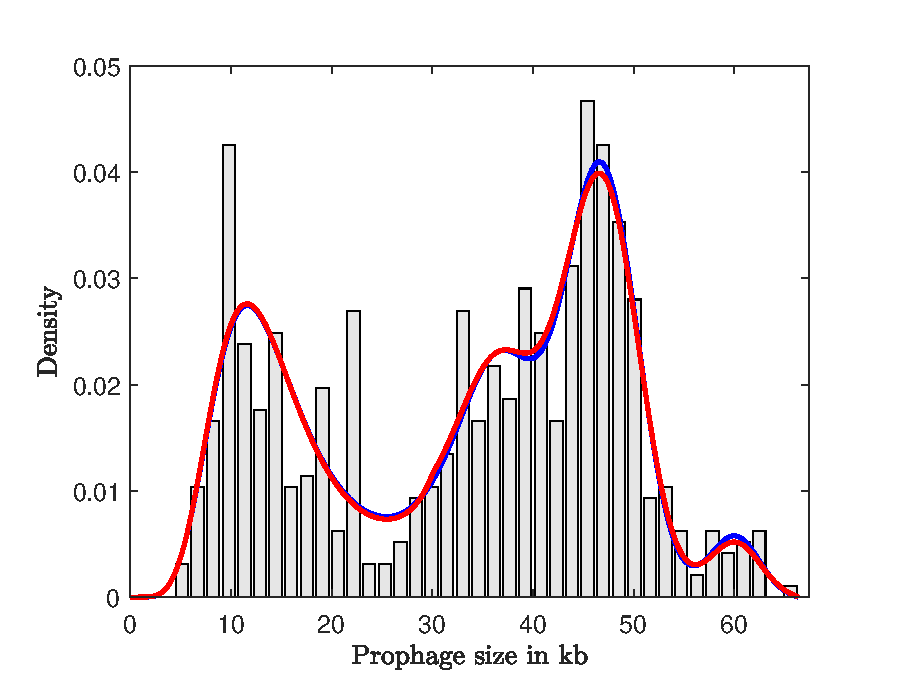
\includegraphics[scale=0.65]{comp_PDF.eps}
% \caption[Results of data fitting are not sensitive to the choice of the parameter $\theta$.]{Results of data fitting are not sensitive to the choice of the parameter $\theta$ representing the genome size of the smallest autonomous temperate phage in kb.  Best fits obtained to Data Set 1 (histogram) for $\theta$ = 20 (blue, solid) and $\theta$ = 30 (red, solid) are indistinguishable.}
% \label{fig:comp_PDF}
% \end{figure}
% \section{Rate parameters}
% We performed a bootstrap sensitivity analysis for all parameters of the model using Data Set 1.  In brief, we assumed that the best fit model for Data Set 1 represented the true distribution, and resampled this true distribution 335 times, each time creating a simulated data set of 624 observed prophage lengths.  We then subjected each of these data sets to the model fitting exercise described in Section 3 of the main text.  Table \ref{table:sens_p} shows the mean and standard deviations for the relative rate parameters of the model (each rate normalized by the induction rate, $r_I$), after the analysis of 335 simulated data sets.  These results indicate that the quantitative conclusions of our work are relatively insensitive to variations in data sampling; the coefficient of variation (standard deviation/mean) of the degradation rate is largest at 16\%.
% %\renewcommand{\baselinestretch}{1}
% \begin{center}
% \begin{table}[t]
% \centering
% \begin{tabular}{ p{1.6cm}p{5cm}p{2cm}p{2cm}p{2.1cm} }
% \hline
% Parameter & Description  & Mean & Standard deviation & Coefficient of Variation  \\
% \hline 
% \\
%  $\alpha $   & Relative rate of lysogeny &     0.2078&          0.0118 & 0.0569\\
%  $r_D$   & Relative rate of degradation &       0.0125&         0.0021 & 0.1644\\
%  $r_S$ &   Relative selection coefficient &    0.5012&     0.0483 & 0.0964\\
% % $r_I$ & Relative rate of induction & 1.0000 &  ---& --- \\
% % \\
%  \hline
% \end{tabular}
% \caption{Sensitivity analysis of rate parameters. }
% \label{table:sens_p}
% \end{table}
% \end{center}
% %\renewcommand{\baselinestretch}{2.0}

% \section{Influx of active phage, $f(x)$}

% In addition, this process produced 335 estimates of the influx distribution $f(x)$.  In Figure \ref{fig:sens_f}, we plot the mean of these functions at every value of $x$ (blue line), plus/minus one standard deviation (grey area).  The best fit $f(x)$ from Data Set 1 is also shown for comparison (red line).  These results indicate that the form of $f(x)$ is very tightly constrained by the data, a result that is perhaps not surprising given the large number of data points.

% \begin{figure}[t]\centering
% 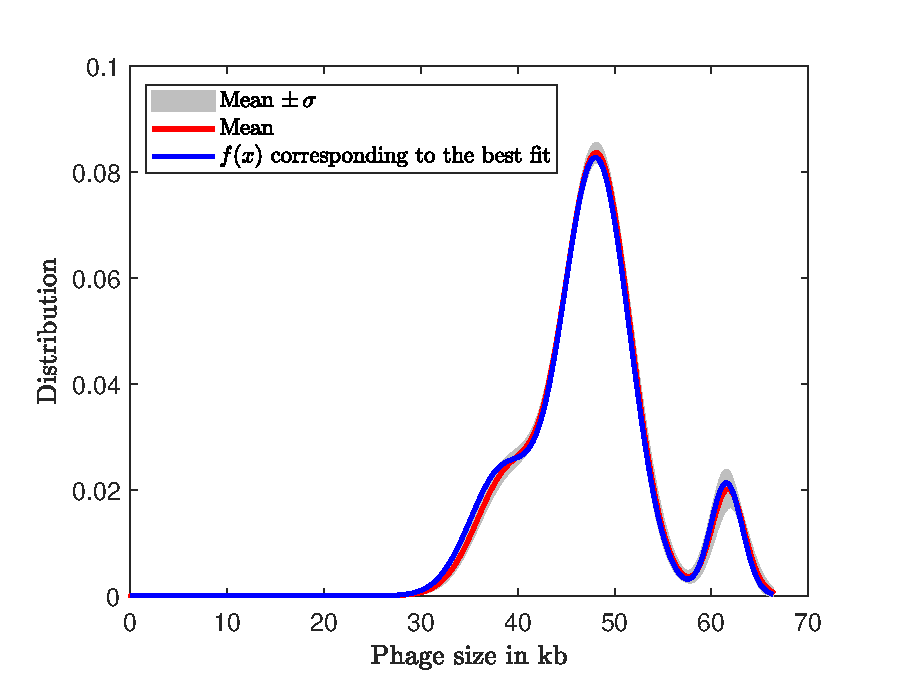
\includegraphics[scale=0.65]{f_sens.eps}
% \caption[Sensitivity analysis of the prophage influx function.]{Sensitivity analysis of the prophage influx function.  The mean (red) and standard deviation ($\sigma$) of best-fit $f(x)$ curves for all simulated data sets are shown, along with the best-fit $f(x)$ function from the true data (blue).  See text for details.}
% \label{fig:sens_f}
% \end{figure}

% \newpage
% \chapter{The influx distribution}

% As described in Section 2.2 of the main text, the function $f(x)$ gives the length distribution for prophages that are newly integrating into bacterial genomes.  Here, we note that this is neither the length distribution of active temperate phages, nor is it the length distribution of inducing phage.

% To clarify, suppose $A(x)$ is the length distribution of active temperate phages. Let $L(x)$ be the average lysogeny probability for a temperate phage of length $x$.  Since $A(x)$ consists of phages of different classes (lambdoid, mu-like, etc.), we expect that $L(x)$ is not constant in $x$.  In this case, the influx distribution  $f(x)$ is given by
% the product $f(x) = A(x)L(x)$.  Thus, unfortunately, we cannot use empirical data describing $A(x)$ to infer $f(x)$.

% Similarly, from the model at steady state, the product $P(x)I(x)$ gives the length distribution of excising prophage.  Suppose $R(x)$ gives the probability that a prophage of length $x$ retains the genes required for re-infection (genes involved in replication, packaging, and adsorption, for example).  If re-infection competent phage enter the lysogenic life cycle with probability $L(x)$, we could also express the influx distribution as $f(x) = P(x)I(x)R(x)L(x)$.  Again, we are unable to use $P(x)I(x)$ to directly infer $f(x)$.

% Despite these limitations, some qualitative features of $f(x)$ and $A(x)$ appear surprisingly robust.  Along with prophage sequences, the length distribution of 68 dsDNA temperate phages infecting enterobacteria are reported in \cite{bobay_pervasive_2014}.  While the weight of the peaks in this multimodal distribution vary, the number and position of the peaks is strikingly similar with our best fit estimate for $f(x)$ for Data Set 1, as shown in Table \ref{table:sens_f}.

% %\renewcommand{\baselinestretch}{1}
% \begin{table}[t]
% \centering
% \begin{tabular}{ p{6cm}p{2cm}p{3cm} }
% \hline
% Feature & Empirical Data & Model Prediction  \\
% \hline
% \\
%  Number of main peaks&     3&          3\\
%   Position of first peak&        $\approx 40$ kb&          $\approx38$ kb\\
%  Position of second peak &    $\approx 45$ kb &          $\approx 48$ kb\\

%  Position of third peak&       $\approx 59$ kb&      $\approx 61$ kb\\
%  \\
%  \hline
% \end{tabular}
% \caption[Comparison of the main features of empirical data describing the length distribution of autonomous dsDNA phages and the best-fit model predictions for the phage influx distribution.]{Comparison of the main features of empirical data describing the length distribution of autonomous dsDNA phages \citep{bobay_pervasive_2014}, and the best-fit model predictions for the phage influx distribution, $f(x)$. }
% \label{table:sens_f}
% \end{table}
% Similarly, we find that $I(x)P(x)$ yields a surprisingly good approximation for $f(x)$, as illustrated in Figure \ref{fig:IP}, again for Data Set 1.  This suggests that most prophage sequences that retain the genes for necessary for excision also retain the genes necessary for re-infection.
% \begin{figure}[t]\centering
% 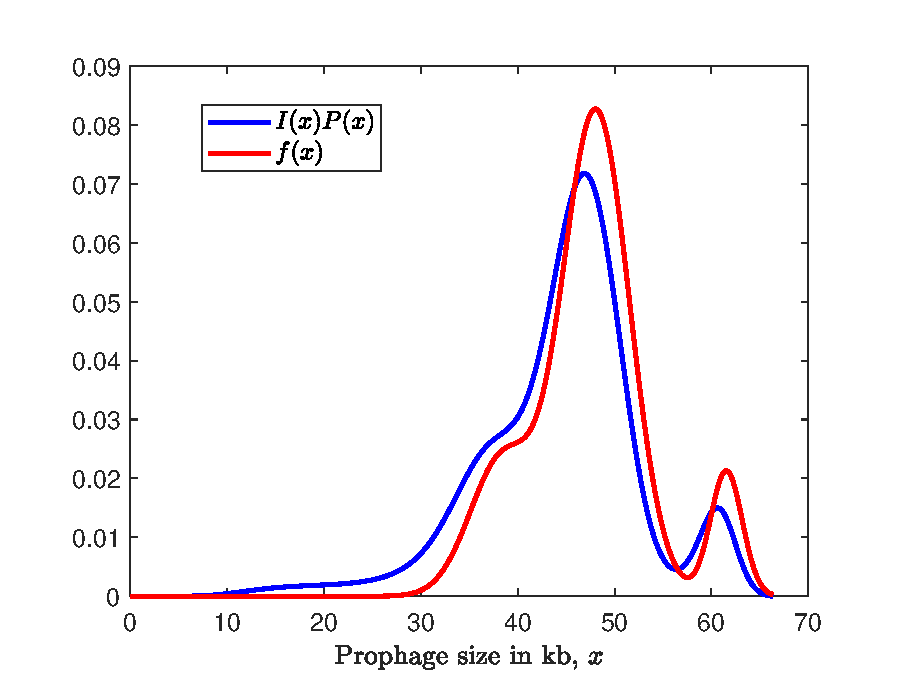
\includegraphics[scale=0.65]{IP.eps}
% \caption[Comparison of best-fit $f(x)$ with the product $P(x)I(x)$.]{Comparison of best-fit $f(x)$ with the product $P(x)I(x)$; results shown for Data Set 1.}
% \label{fig:IP}
% \end{figure}
% \end{appendices}

\chapter{The genetic repertoire of prophages}
 Bacterial genome sequencing has revealed that prophages – the functional or cryptic genome sequences of temperate bacteriophages – are far more numerous than previously recognized.  Prophages are subject to mutational degradation, but they may also be maintained by selection if they confer benefits to their bacterial hosts; these evolutionary forces will have different effects on prophage genes of different function. In this chapter, we examine the distributions of 53,356 annotated prophage genes identified in 1384 prophage sequences, comparing the gene repertoires of intact and incomplete prophages.  These data indicate that genes involved in the replication, packaging, and release of phage particles have been preferentially lost in incomplete prophages, while transposase and integrase genes are significantly enriched.  In this chapter, we also developed mathematical and computational models to test how evolutionary forces affect prophage gene repertoires.  These approaches demonstrate that genes involved in phage lytic function are preferentially lost, resulting in shorter prophages that often retain genes that benefit the host.  Meanwhile, the model suggests that the enrichment of transposase sequences in shorter prophages is likely due to their role in disruption of phage lysis genes and generation of cryptic prophages that cannot harm their hosts.  Overall, we show that variation in positive and negative selection on different prophage gene classes explains the diversity of prophage genome structures, including the evolution and maintenance of cryptic and domesticated prophage sequences. 
\section{Introduction}
Bacteriophages, viruses that infect bacteria, are the most prevalent life form on the planet, vastly outnumbering both their bacterial hosts and all other life forms combined \cite{bergh_high_1989, rohwer_global_2003, clokie_phages_2011}.  As lethal pathogens, lytic bacteriophages typically reproduce in large numbers, causing the death of their hosts in the process.  Temperate phages, however, are so-named because they also have the ability to integrate their genetic code into the host cell DNA, leaving the host cell unharmed.  Once integrated, these viral sequences can persist as \emph{prophages} for many bacterial generations, being replicated as part of the host cell genome during cellular fission.

While integrated in the bacterial genome, prophage sequences are subject to selection, mutation, and horizontal gene transfer (HGT).  A wealth of recent evidence argues for the role of positive selection in the maintenance of prophages which confer benefits such as immunity against other infecting phages, antibiotic resistance, resistance to environmental stress and numerous virulence factors \cite{harrison_ecological_2017}.  Mutation in bacterial genomes is biased toward deletion \cite{kuo_deletional_2009,mira_deletional_2001, danneels_patterns_2018}, and thus prophage sequences are subject to mutational degradation over long time scales.  In addition, some families of prophages carry transposase genes, enabling replicative (copy-and-paste) transposition of the prophage sequence to other locations in the bacterial genome. 

If a prophage retains the functional genes required for replication, packaging and cellular lysis, the prophage sequence can initiate \emph{induction}, a process in which the prophage resumes its role as a lethal pathogen, produces a large number of daughter phage, and kills the host.  Spontaneous induction rates  are in the range of $10^{-5}$ to $10^{-3}$ per bacterial generation \cite{little_robustness_1999,zong_lysogen_2010}, but can be substantially increased if the bacterial host cell is in stress \cite{alexeeva_spontaneously_2018}.

Genome sequencing and comparative genomics have recently revealed that prophages are far more numerous and more widely-shared across bacterial genomes than previously recognized \cite{costa_genomic_2018, mottawea_salmonella_2018}.  In addition, four recent studies have independently reported that the distribution of prophage lengths is bimodal \cite{bobay_pervasive_2014, brueggemann_pneumococcal_2017, crispim_screening_2018, leplae_aclame:_2010}, a phenomenon that may be explained by the balance between selection for prophage maintenance (via beneficial effects of prophage genes) and selection against prophage (via harmful effects of induction and cell lysis) \cite{khan_quantifying_2019}.
These fundamental evolutionary forces will differentially affect prophage genes of different function.  For example, while short deletions might affect all prophage genes, positive selection will affect only those prophages that carry genes of benefit to their host; negative selection (via induction) will affect only prophages that carry functional induction genes.  Thus, prophages of differing lengths, or differing degrees of integrity when compared to the ancestor phage genome, may carry different genetic repertoires -- signatures of the evolutionary forces in play. Indeed, tail fiber and integrase coding sequences are significantly enriched in small prophages (Figure S1, \cite{bobay_pervasive_2014}), but little else is understood about the gene repertoires of intact or degraded (incomplete) prophage sequences. 

In this contribution, we examine the distributions of prophage genes identified in publicly available genome sequences, comparing the gene repertoires of intact and incomplete prophages.  To better understand these results, we also develop both a mathematical and computational model describing the fates of distinct gene classes in prophages. 
Our results support the roles of both positive and negative selection in maintaining prophage sequences with diverse genetic repertoires, and offer explanations for both the enrichment and loss of specific gene functions in cryptic prophages.

\section{Gene repertoire of sequenced prophages}
We investigated bacterial genomes studied in two previously published data sets \cite{bobay_pervasive_2014,leplae_aclame:_2010}, using the PHASTER interface \cite{arndt_phaster:_2016} for rapid prophage identification and gene annotation.  Data Set 1, originally studied by Bobay et al. \cite{bobay_pervasive_2014}, includes 624 prophages from 85 bacterial genomes; these prophage sequences contain 24,877 annotated genes.  Data Set 2, as studied by Leplae et al. \cite{leplae_aclame:_2010}, includes 760 prophages  from 306 bacterial genomes, with 28,479 annotated genes.  For the 13 phage gene functions listed in Table \ref{tab:genes}, we tracked the number of prophages identified as containing at least one gene of that class.  We further partitioned these data based on whether the prophage sequence was classified as ``intact", ``questionable" or ``incomplete" by the PHASTER algorithm.

\renewcommand{\baselinestretch}{1}
\begin{table}
  \centering
  \renewcommand{\arraystretch}{2}
  \begin{tabular}{|p{2cm}|c|c|c|c|c|c|c|c|}
    \hline
    \multirow{3}{2cm}{\textbf{Gene}} & 
    \multicolumn{6}{c|}{\textbf{Number of prophages containing a gene of this type}}\\ \hline
    & \multicolumn{3}{|c|}{\textbf{Count in Data Set 1}} & \multicolumn{3}{c|}{\textbf{Count in Data Set 2}}\\
    \cline{2-7}  
    & \textbf{Intact} & \textbf{Questionable} & \textbf{Incomplete} & \textbf{Intact} & \textbf{Questionable} & \textbf{Incomplete}\\
    %\hhline{~--}
    \hline
    terminase & 317 & 25 & 14 &292 &53 &58  \\ \hline
    portal & 277 & 9 & 3 &283   &67 &48  \\ \hline
    head & 299 & 16 & 25 &281  &79 &86  \\ \hline
    injection & 14 & 0 & 2 & 4 & 0 & 0 \\ \hline
    tail & 413 & 46 & 86 &419  &116 &141  \\ \hline
    protease & 82 & 3 & 5 &72  &12 &22  \\ \hline
    transposase & 195 & 32 & 75 & 190 & 173 & 144 \\ \hline
    integrase & 346 & 54 & 85 &  312 &94 & 165 \\ \hline
    lysis & 226 & 19 & 11 & 52 & 6 & 6  \\ \hline
    plate & 121 & 5 & 0 &143  & 20 & 28 \\ \hline
    capsid & 225 & 14 & 18 &233  & 50 & 40  \\ \hline
    lysin & 235 & 17 & 19 &165  & 32 &22  \\ \hline
    flippase & 2 & 0 & 20 & 0 & 1 & 4  \\ \hline \hline
    \textbf{Total} & 2752 & 240 & 363 & 2446 & 603 & 764  \\ \hline
  \end{tabular}
  \caption{ The genetic repertoire of prophages in Data Set 1 and Data Set 2.}
\label{tab:genes}
\end{table}
\renewcommand{\baselinestretch}{2}

Figure \ref{fig:data4} plots the frequency of each gene class in intact ($f_{\mbox{int}}$), questionable and incomplete ($f_{\mbox{inc}}$) prophages.  The genes are ordered left to right according to their degree of enrichment in incomplete prophages; due to small numbers, gene types that constituted less than 1\% of the data have been excluded.  These results are summarized in the lower panels of Figure \ref{fig:data4}, which show the percent change in gene frequency between incomplete and intact prophages, that is:
\[
\% \mbox{ change} = 
\frac{100 ( f_{\mbox{inc}} - f_{\mbox{int}} )}
{ f_{\mbox{int}} } \,\,.
\]
Positive values of \% change thus indicate genes that are relatively enriched in incomplete prophages, while negative values indicate genes that are preferentially lost.

\renewcommand{\baselinestretch}{1}
\begin{table}
  \centering
  \renewcommand{\arraystretch}{2}
  \begin{tabular}{|l|c|c|c|c|c|c|}
    \hline
    \multirow{3}{*}{} & 
    \multicolumn{6}{c|}{\textbf{Number of transposase genes identified}}\\ \hline
    & \multicolumn{3}{|c|}{\textbf{Count in Data Set 1}} & \multicolumn{3}{c|}{\textbf{Count in Data Set 2}}\\
    \cline{2-7}  
    & \textbf{Intact} & \textbf{Questionable} & \textbf{Incomplete} & \textbf{Intact} & \textbf{Questionable} & \textbf{Incomplete}\\
    \hline
    IS transposase & 174 & 34 & 76 & 459 & 90 & 109 \\ \hline
        non-IS transposase & 278 & 37 & 88 & 464 & 101 & 99\\ \hline
    \hline
    \textbf{All phage proteins} & 21054 & 2271 & 1552 & 19250 & 5097 & 4132 \\ \hline
  \end{tabular}
  \caption{ The distribution of transposase genes identified in Data Set 1 and Data Set 2.}
  \label{tab:transp}
  \end{table}
  \renewcommand{\baselinestretch}{1}

\begin{figure}
    \centering
    \begin{subfigure}[t]{0.50\textwidth}
    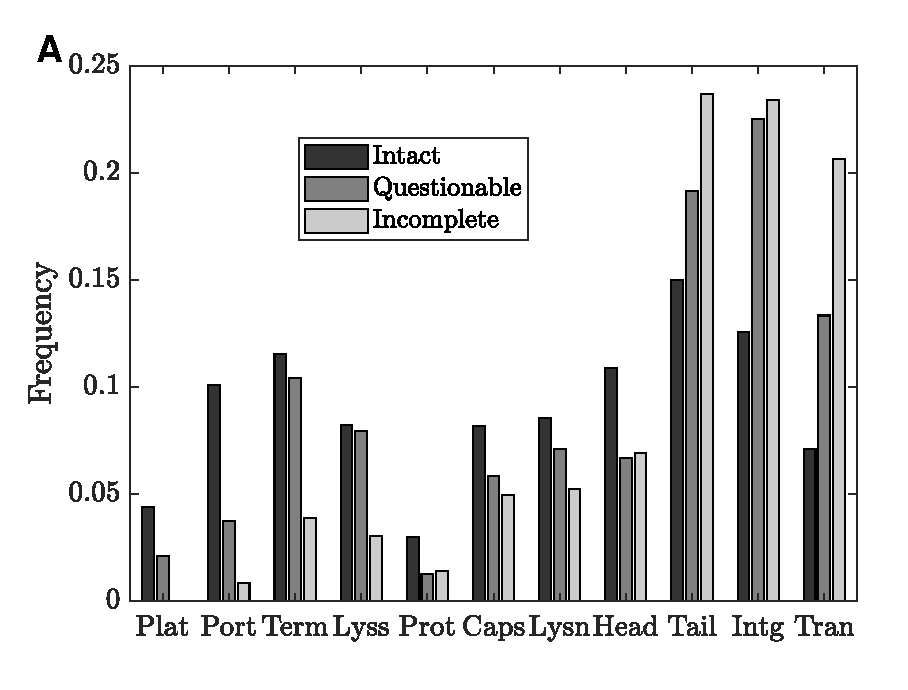
\includegraphics[scale=0.50]{bobay1}
     \end{subfigure}\hfill
     \begin{subfigure}[t]{0.50\textwidth} 
    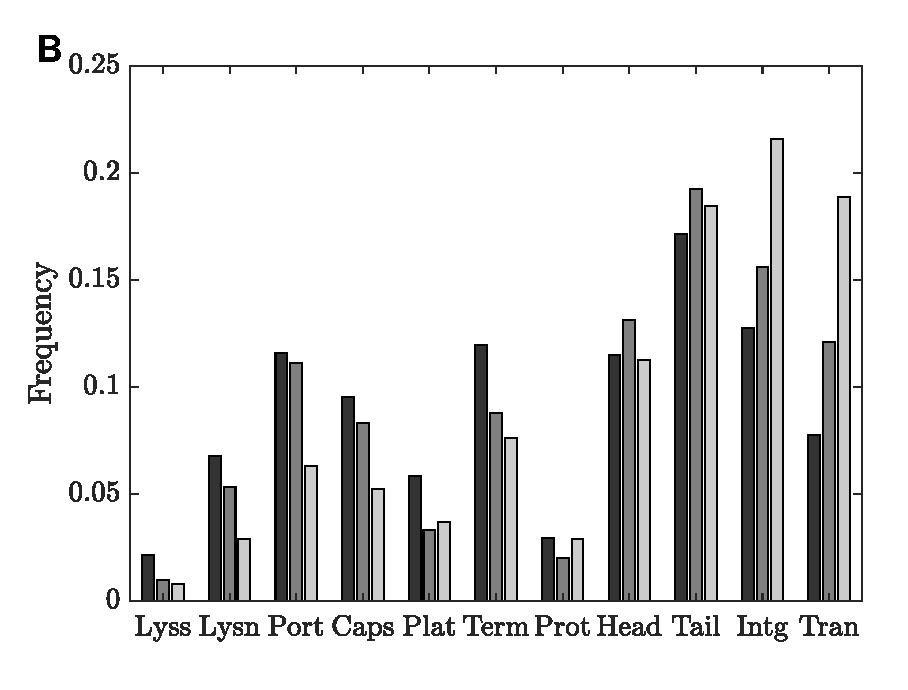
\includegraphics[scale=0.50]{aclame1}
    \end{subfigure}\hfill
         \begin{subfigure}[t]{0.50\textwidth}
    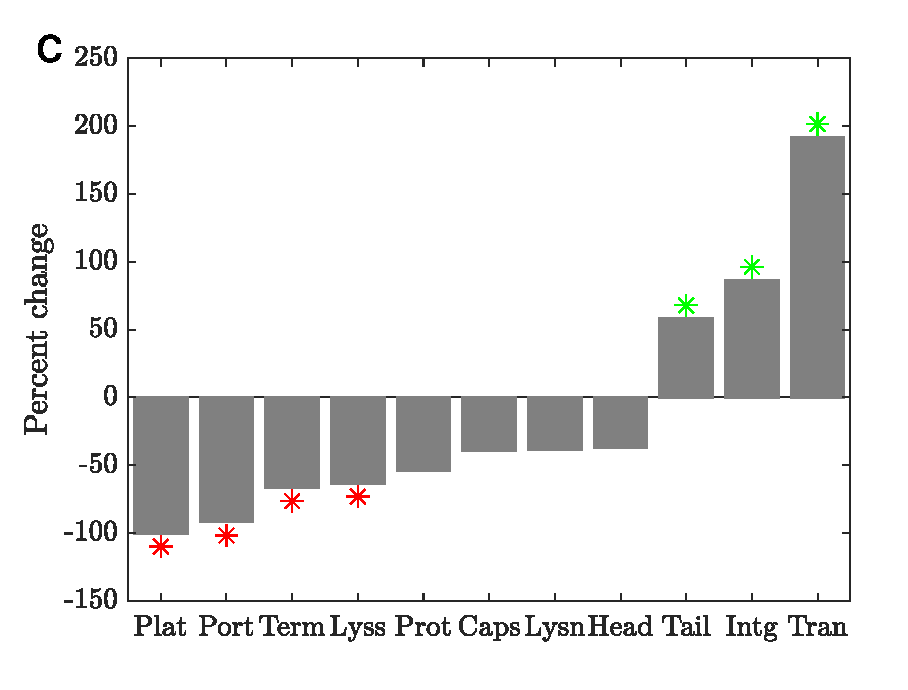
\includegraphics[scale=0.50]{bobay2}
     \end{subfigure}\hfill
     \begin{subfigure}[t]{0.50\textwidth} 
    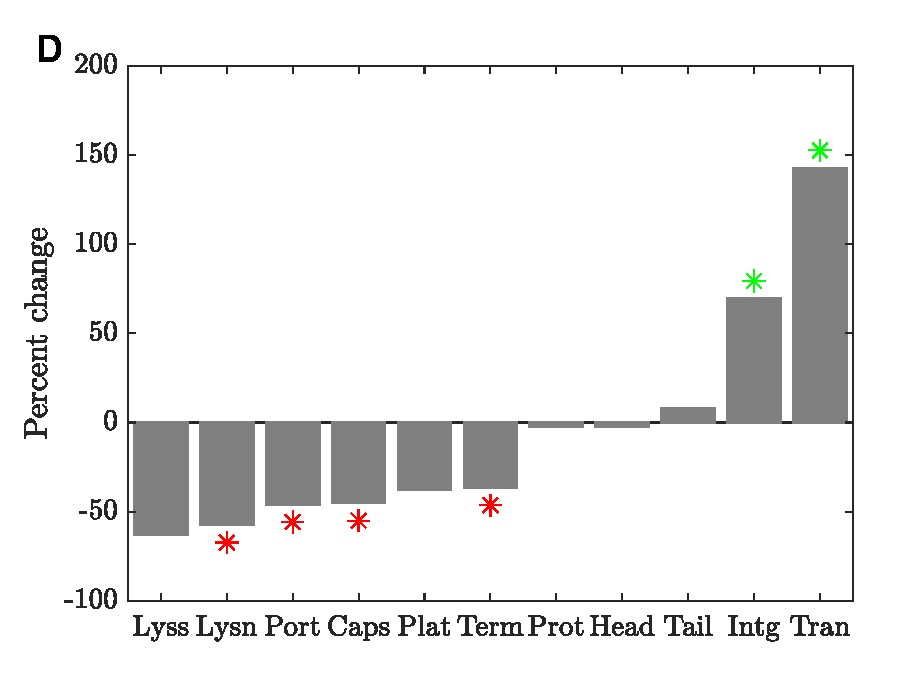
\includegraphics[scale=0.50]{aclame2}
     \end{subfigure}\hfill
    \caption[Changes in prophage gene frequencies, for intact, questionable and incomplete prophages.]{Changes in prophage gene frequencies, for intact, questionable and incomplete prophages.  (A) The frequency of each gene class identified in Table \ref{tab:genes} in prophages from Data Set 1 \cite{bobay_pervasive_2014}, for prophages identified as intact, questionable or incomplete.  Gene classes that constituted less than 1\% of the data have been excluded. Gene classes are ordered by the percent change in frequency (degree to which they are enriched in incomplete prophages, see panel C.) (B) Gene frequencies as in panel A, but for Data Set 2 \cite{leplae_aclame:_2010}.  (C) Percent change in gene frequency; the frequency of each gene class in incomplete prophages is compared to the baseline frequency of that class in intact prophages.  Frequencies that were significantly lower (red) or higher (green) than expected by chance with a two-sided 5\% significance threshold are indicated by stars.  Thus red stars indicate gene classes that are preferentially lost, while green stars indicate classes that are enriched in short prophages.  (D) Percent change in gene frequency for Data Set 2.} 
\label{fig:data4}
\end{figure}

To evaluate the statistical significance of these results, for each gene type we use the same number of identified genes (e.g. 317+25+14 = 356 for terminase in Data Set 1), and randomly assign the genes to one of the three prophage classes.  Because intact prophages in the dataset contain more genes than incomplete prophages, we also preserve the proportion of genes assigned to each class.  Thus in randomly assigning genes to prophage classes, we assign 2752/(2752+240+363) = 82\% of genes to intact prophages in Data Set 1, for example, while only
363/(2752+240+363) = 11\% are assigned to
incomplete prophages.

We computed the percent change in gene frequency for these bootstrapped data as described above, and repeated this procedure 10,000 times.  Stars in the lower panels of Figure \ref{fig:data4} indicate \% change values in the data that were lower than the 2.5 percentile or higher than the 97.5 percentile in the bootstrapped distributions.

These results reveal several features that are conserved between data sets.  We note that lysis or lysin genes, as well as portal and terminase proteins, are preferentially lost in incomplete prophages.  In contrast, transposase and integrase genes are substantially enriched.  We explore these results further in both the computational and mathematical models described in the sections to follow.

In light of the striking enrichment of transposase genes in incomplete prophages, we examined the transposase annotations in greater detail.  For each prophage in the dataset, we downloaded the coding sequences and the BLAST hits identified for each coding sequence by PHASTER \cite{arndt_phaster:_2016}.  We counted the number of coding sequences with a BLAST hit annotated as an insertion sequence (IS) transposase (e.g. ``IS3 transposase B''), as well as those annotated as a transposase but without a BLAST hit to an IS.  As a control, we also counted the total number of proteins identified as a ``phage hit protein'' by PHASTER in each data set.  

As shown in Table \ref{tab:transp}, IS transposases account for 41.4\% of the transposase sequences identified in Data Set 1, and 49.8\% of those in Data Set 2.  In Data Set 1, the frequency of IS transposases (calculated as the fraction of all phage proteins identified) is enriched 4.9-fold in incomplete prophages as compared to intact prophages; the frequency of non-IS transposases also increased but to a lesser degree (3.3-fold).  In Data Set 2, the frequency of IS transposases increased by 10\% in incomplete prophages, while non-IS transposases were reduced by 0.6\%.  Thus in both data sets, the frequency of IS transposases is enriched in incomplete prophages, and enriched to a greater degree than non-IS transposases.  As discussed further below, this suggests that the enrichment of transposase sequences in incomplete prophages may be due to the disruption of essential prophage functions due to IS insertion; in other words, the presence of the IS transposase has rendered the prophage cryptic.


\section{Analytical model of prophage gene content}

To investigate the preferential loss or maintenance of specific classes of phage genes in prophage sequences over time, we developed a mathematical model.  The model, although simplified, allows us to predict the effects of key parameters on the longterm genetic repertoire of prophages.

The model tracks a population of bacterial genomes, which contain prophages with genes in three possible types -- beneficial genes, excision genes and re-infection genes. Beneficial genes are genes that confer a selective advantage to the host, thus increasing the prophage population through vertical transmission. Biological examples of beneficial genes include host virulence factors that help the bacterial cell during colonization of its host (for example phage lambda's \emph{lom} gene). In contrast, excision genes are the genes involved in prophage induction into the lytic cycle, which leads to the death of the host cell. Examples of excision genes include lambda's \emph{O} and \emph{P} genes, which switch on the lytic cycle by commandeering the host's DNA polymerase. Phage induction will typically lead to bacterial cell death regardless of the quantity or quality of phage progeny.  Phage progeny success is determined by the phage's re-infection genes, comprising the genes required for phage genome replication, packaging, lysis, transmission to a new host, and reestablishment of lysogeny.  This re-infection class, in particular, includes a large number of genes of different function; yet their net effect, taken together, is to increase the prophage population through horizontal transmission.



In the simplified model, we consider a full prophage as one containing just three `genes', one of each class.  Here, we can think of a `gene' as a full functional complement of the underlying sequences required for each function.  We denote the frequency of full prophages in the population at time $t$ as $P_{1 1 1}(t)$. More generally, we use the notation $P_{ber}$ to represent the frequency of prophages with (1) or without (0) the beneficial, excision or re-infection genes respectively.  For completeness, the model also includes a population $P_{000}$ corresponding to bacterial genomes in which the prophage has been completely lost.  Note that in the computational model to follow, we will both expand these gene classes and include multiple genes per class.

The analytical model includes the following processes:

{\bf Degradation}:  Each gene in each prophage in the population is lost (gene deletion) at rate $r_{D}$. For example, the frequency of $P_{111}$ is lost at overall rate $3r_D$, contributing at rate $r_D$ to each of the populations $P_{011}$, $P_{101}$ and $P_{110}$.

{\bf Induction}: If a bacterial genome contains a prophage which carries the excision gene, the prophage induces at rate $r_I$ and the bacterium is lost from the population.

{\bf Re-infection}:  Prophages that carry both the excision and re-infection genes ($P_{111}$ and $P_{011}$) reproduce (create copies of themselves in new bacterial genomes), through lysis, re-infection and lysogeny, at rate $r_L$.  %Note that in the mathematical model, new (full length) prophages are not added to the prophage population from an external pool.
    
{\bf Selection}: To model the potential selective benefit conferred by the prophage, we assume that bacterial populations that carry the beneficial prophage gene grow at per capita rate $r_S$.

These assumptions yield the following system of ordinary differential equations, illustrated as a schematic in Figure \ref{fig:schematic}:

\begin{eqnarray}
\frac{d P_{1\,1\, 1}}{dt} &=& (r_L  +r_{S} - 3 r_{D} - r_{I}) P_{1\,1\, 1} - \phi P_{1\,1\,1} \nonumber\\
\frac{d P_{0\,1\, 1}}{dt} &=& (r_L - 2 r_{D} - r_{I}) P_{0\,1\, 1}+ r_{D}P_{1\, 1\, 1} - \phi P_{0\,1\,1}  \nonumber\\
\frac{d P_{1\,0\, 1}}{dt} &=& (r_{S} - 2 r_{D}) P_{1\,0\, 1} + r_D P_{1\,1\, 1}- \phi P_{1\,0\,1} \nonumber\\
\frac{d P_{1\,1\, 0}}{dt} &=& (r_{S} - 2 r_{D} - r_{I}) P_{1\,1\, 0}+ r_{D} P_{1\,1\, 1} - \phi P_{1\,1\,0}  \nonumber\\
\frac{d P_{0\,0\, 1}}{dt} &=& (- r_{D}) P_{0\,0\, 1} + r_{D} P_{0\,1\, 1} +r_{D} P_{1\,0\, 1}- \phi P_{0\,0\,1} \nonumber\\
\frac{d P_{0\,1\, 0}}{dt} &=& (- r_{D} - r_{I}) P_{0\,1\, 0} + r_{D} P_{0\,1\, 1} +r_{D} P_{1\,1\, 0}- \phi P_{0\,1\,0} \nonumber\\
\frac{d P_{1\,0\, 0}}{dt} &=& (r_{S} - r_{D}) P_{1\,0\, 0}+ r_{D} P_{1\,0\, 1} +r_{D} P_{1\,1\, 0}- \phi P_{1\,0\,0}\nonumber\\
\frac{d P_{0\,0\, 0}}{dt} &=&  r_{D}( P_{1\,0\, 0} + P_{0\,1\, 0} + P_{0\,0\,1})
- \phi P_{0\,0\,0}\,\,.
\label{systemC}
\end{eqnarray} 
Here, terms involving $\phi$ simply ensure that the frequencies sum to unity at all times, with $\phi$ defined as:
\[\phi = (r_L  +r_{S} - r_{I}) P_{1\,1\, 1} +  (r_L - r_{I}) P_{0\,1\, 1} + r_{S} P_{1\,0\, 1} + (r_{S}- r_{I}) P_{1\,1\, 0} - r_{I} P_{0\,1\, 0} + r_{S} P_{1\,0\, 0}\,\,.
\]

\begin{figure}[H]
 \centering
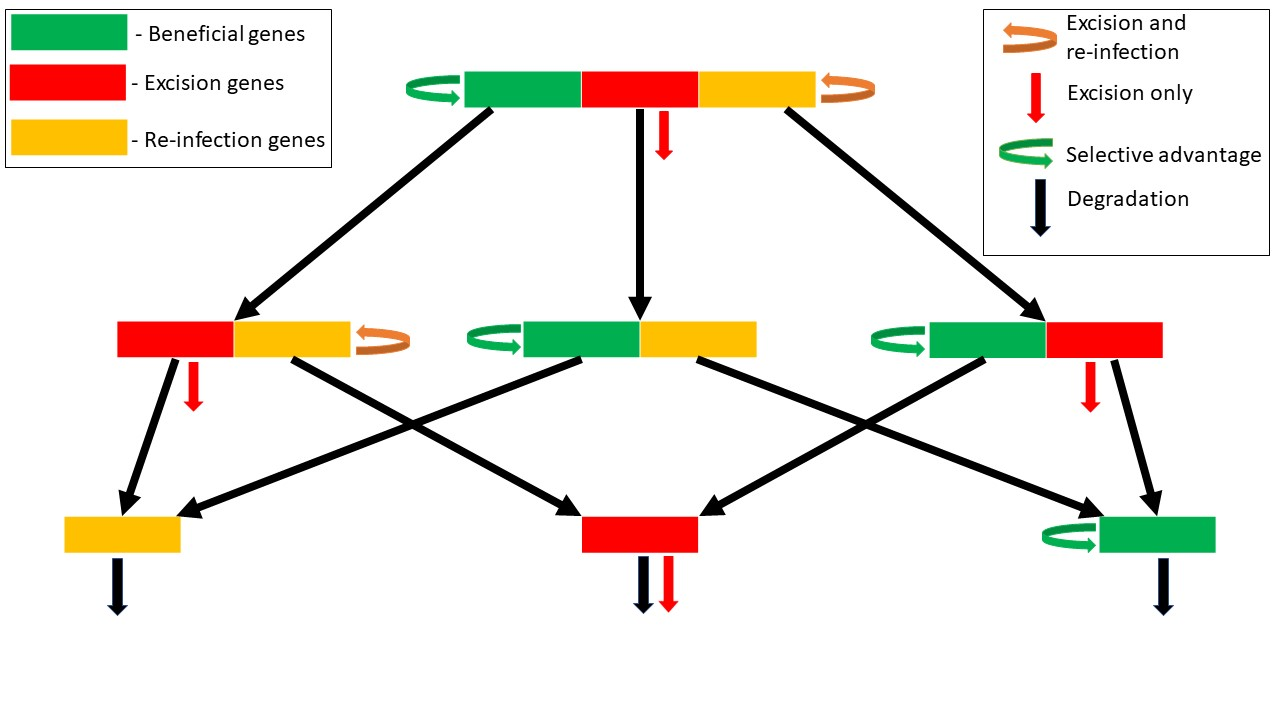
\includegraphics[width=15cm]{Model}
\caption{Schematic diagram of the mathematical model.}
\label{fig:schematic}
\end{figure}

A detailed analysis of the equilibria and stability of this 8-dimensional model is provided in the Supplementary Material. From this analysis, we find four possible longterm outcomes: (1) equilibrium $E_0$, in which all prophage genes are lost; (2) equilibrium $E_B$, in which both excision and re-infection genes are lost, but beneficial genes persist.  This equilibrium reflects complete domestication of the prophage; (3) equilibrium $E_{ER}$, in which beneficial genes are lost but both excision and re-infection genes persist. This corresponds to a virulent prophage that does not contribute to host fitness; (4) equilibrium $E_A$, in which all three types of genes persist.

As described in the Supplementary Material, two critical conditions are sufficient to determine the long-term behaviour of the prophage gene distribution.

Condition 1: $r_S> r_D$. Note that $r_S$ is the rate at which a beneficial gene produces a new copy of itself, while $r_D$ is the rate at which a beneficial gene is lost, which occurs through mutational degradation.  Thus $r_S>r_D$ implies that on average, a beneficial gene makes more than one copy of itself before it is lost: beneficial genes persist.

Condition 2: $r_L> 2r_D + r_I$.  Similarly, the combination of an excision and a re-infection gene, co-occuring on a prophage, is able to produce a new copy of itself at rate $r_L$. These genes may be lost through induction, but also lost if either gene is degraded by mutation, so the total rate of loss is $2r_D + r_I$.  Thus this gene combination can persist if $r_L>2r_D + r_I$.

The predicted behaviour of the mathematical model can therefore be summarized as shown in Table \ref{tab:conditions}.

\renewcommand{\baselinestretch}{1}
\begin{table}
\centering
\begin{tabular}{| c | c | c |}
\hline
{\bf Longterm prediction} & B genes do not persist & B genes persist \\
Condition & $r_S<r_D$ & $r_S > r_D$ \\
\hline
ER genes do not persist & {\bf extinction} &  {\bf domestication} \\
$r_L < 2r_D + r_I$ &  $E_0$ & $E_B$ \\
\hline
ER genes persist & {\bf virulence} & {\bf persistence} \\
$r_L > 2r_D + r_I$ &  $E_{ER}$ & $E_A$ \\
\hline
\end{tabular}
\caption{Conditions determining which classes of prophage genes persist longterm.}
\label{tab:conditions}
\end{table}
\renewcommand{\baselinestretch}{2}

In Figure \ref{fig:mathresults}, we illustrate the approach of System \ref{systemC} to each of these four equilibrium states, for appropriate parameter values.  To simplify the presentation, we plot the the average number of genes of each type carried per prophage, where for example the average number of beneficial genes per prophage is given by $P_{111} + P_{110} + P_{101} + P_{100}$.  Equivalently, this is the fraction of prophages that carry the beneficial gene.

 \begin{figure}[H]
    \centering
     \begin{subfigure}[t]{0.50\textwidth} 
    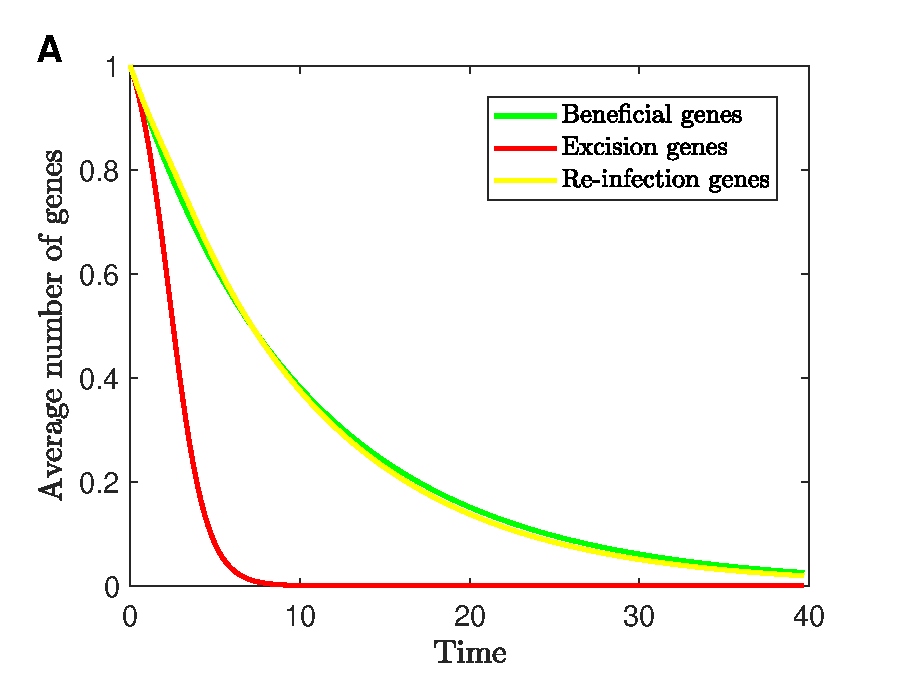
\includegraphics[scale=0.50]{triv}
     \end{subfigure}\hfill
         \begin{subfigure}[t]{0.50\textwidth}
    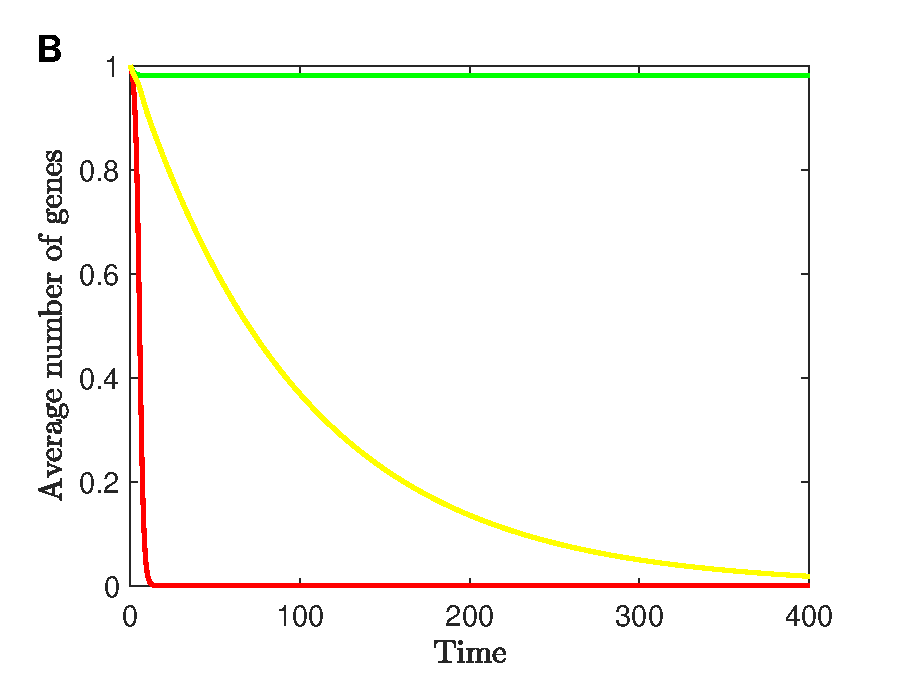
\includegraphics[scale=0.50]{E_b}
    \end{subfigure}\hfill\\  \begin{subfigure}[t]{0.50\textwidth}
        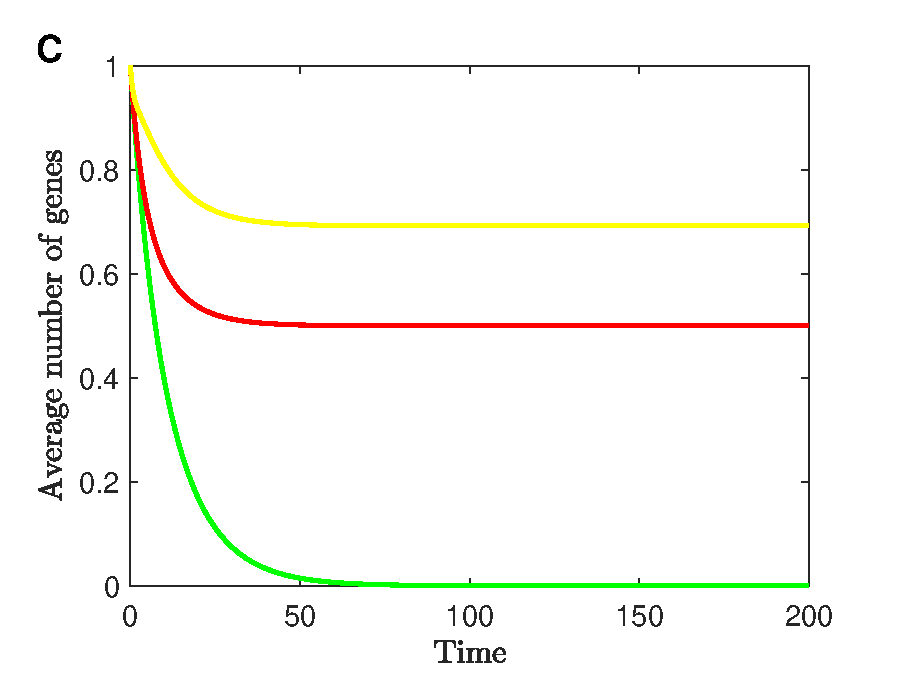
\includegraphics[scale=0.50]{E_li}
    \end{subfigure}\hfill   \begin{subfigure}[t]{0.50\textwidth}
    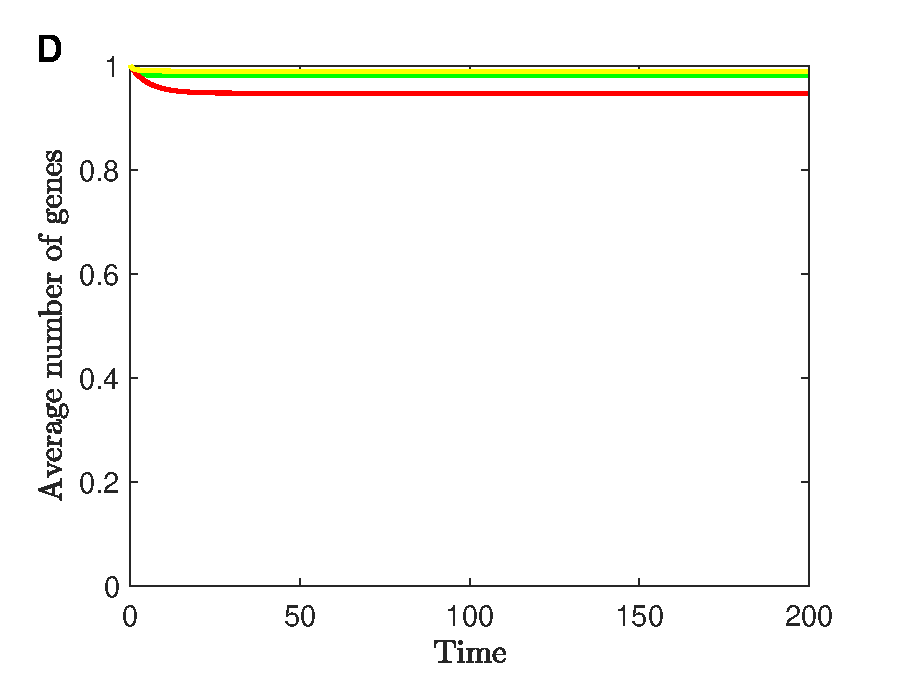
\includegraphics[scale=0.50]{E_lib}
    \end{subfigure} 
     \caption[Numerical integration of the analytical model.]{Numerical integration of the analytical model, showing System \ref{systemC} converging toward four possible equilibria: (A) {\bf Extinction}, $E_0$($r_S = 0.01 , \, r_D =0.1 , \, r_L =0.2 \, $);  (B) {\bf Domestication}, $E_B$ ($r_S = 0.52 , \, r_D =0.01 , \, r_L =0.2  $); (C) {\bf Virulence}, $E_{ER}$ ($r_S = 0.02 , \, r_D =0.1 , \, r_L =1.3  \, $); (D) {\bf Persistence}, $E_A$ ($r_S = 0.52 , \, r_D =0.01 , \, r_L =1.2  \, $).  In all cases, $r_I=1$.}
     \label{fig:mathresults}
     \end{figure}
\section{Gene Repertoire Simulations}

We also developed a computational model which is able to describe the gene content of prophage sequences in greater detail.  Here, we assume that prophages exist in a population of bacterial genomes that are linked by both cellular reproduction (vertical transmission of the prophage) and horizontal gene transfer (horizontal transmission).  We can vary the initial conditions such that all or only some of the bacterial genomes initially carry prophages.  Bacterial genomes that carry inducible prophage sequences may be lost through induction and lysis, whereas bacterial genomes that carry beneficial prophage sequences may be preferentially copied to the next generation.  We describe these steps in detail below.

Each prophage sequence may contain genes of the following four types: excision genes, re-infection genes, beneficial genes and neutral genes.  A full prophage carries $n_E$ excision genes, $n_R$ re-infection genes, $n_B$ beneficial and $n_N$ neutral genes.  We include mutational degradation and also include the possibility that an insertion sequence (or other transposable element) could disrupt the prophage genome. 

We track the presence or absence of each gene in each prophage sequence. A discrete timestep in the simulation corresponds to a bacterial generation time.  The rates of the underlying processes, however, are expressed in units of the ``prophage generation time", that is, the average time that a single prophage sequence is maintained in a bacterial genome before induction \cite{khan_quantifying_2019}.  Since the bacterial generation time, $\Delta t$, is much shorter than the prophage generation time, if a process occurs at rate $r$ per prophage generation, the probability that it occurs in timestep $\Delta t$ is small and well-approximated by $r \Delta t$.

The following processes are included in the model, with parameters as described in Table \ref{tab:params}:

{\bf Degradation}:  In each time step, each gene in each prophage in the population is removed (gene deletion) with probability $r_{D} \Delta t $. 

{\bf Induction}: If a prophage carries all $n_E$ excision genes, it may induce with probability $r_I \Delta t$.  When a prophage induces, it is removed from the population.  We thus assume that all $n_E$ excision genes are required for excision and death of the host cell.  Note that we ignore polylysogeny, that is, we make the simplifying assumption that excision and cell death affect only the excising prophage.

{\bf Re-Infection}:  To simulate the process of lysis followed by re-infection and lysogeny, a copy of any prophages that carry all $n_E$ excision genes \emph{and} all $n_R$ re-infection genes may be added to the prophage pool with probability $r_L \Delta t$.
Thus, full complements of both the excision and re-infection genes are required to reinfect.
In addition, in some simulations new (full length) prophages are added to the prophage pool with probability $r_F \Delta t$.  This might occur for example if there is an influx of prophages to the local population from an external pool.
    
{\bf Selection}: Copies of existing prophages are also added to the population at rate $r_S \Delta t\,n_b/n_B$.  Here $n_b$ is the number of beneficial genes carried by the prophage, and $r_S$ is the maximum selective benefit provided to the host cell if the prophage contains all $n_B$ beneficial genes. 

{\bf Population regulation}: We consider a pool of prophages that exists within a bacterial population that cannot grow unbounded.  To regulate the population size, if the current population size $N$, is greater than the bacterial carrying capacity, $K$, each bacterial genome is copied into the subsequent generation with probability $K/N$.
    
While all of our simulation studies include the processes described above, in some simulations we also explored the impact of disruption by transposable elements (TEs, such as bacterial insertion sequences) as follows.

{\bf TE disruption}: Motivated by the observed frequencies of IS transposase sequences in incomplete prophages, we include the possibility of TE disruptions in prophage genes.  For each gene in each timestep, a TE disruption may occur with probability $r_T \Delta t$.  When this occurs, we assume that gene function has been disrupted: if a beneficial gene has been disrupted, the gene confers no benefit to the host thereafter; if a gene required for excision or re-infection is disrupted, the prophage is no longer able to kill the host or re-infect respectively.  Thus TE disruptions have the same effect as gene deletions, but leave a signature of TE sequences in the prophage genome.  

We wondered whether it was reasonable to include TE disruptions in the model, since their rates might be negligible relative to mutational degradation. Rates of base pair substitutions in {\it E. coli} K12 have been estimated to be on the order of $2\times10^{-10}$ per nucleotide, per generation \cite{foster_determinants_2015}.  Multiplying by 1.2 kb per prophage gene \cite{khan_quantifying_2019} yields an estimate of $2.4\times10^{-7}$ base pair substitutions, per prophage gene, per bacterial generation.  Presumably only a fraction of base pair substitutions result in loss of function.  In addition, small indels are estimated to occur at about one tenth of this rate \cite{foster_determinants_2015}.  Thus taking in {\it E. coli} as a model organism, rates of prophage gene degradation through mutation (base pair substitution and short indels) might occur on the order of $10^{-7}$ or $10^{-8}$ per gene per generation.

In comparison, rates of transposition, for 5 insertion sequences in {\it E. coli} K12, have been estimated to be about $1\times10^{-5}$ per element per generation \cite{sousa_rates_2013}; this includes both copy-and-paste and cut-and-paste transpositions.  The ancestral genome in this mutation accumulation study carried a total of 33 copies of these ISs, yielding an overall transposition rate of $3.3\times10^{-4}$ transpositions per generation.  Given that a typical prophage gene comprises 1.2 kb \cite{khan_quantifying_2019} of a 4.6 Mb {\it E. coli} genome, we arrive at an estimated transposition rate of $8.6\times10^{-8}$ per prophage gene, per bacterial generation, similar to our estimate for gene loss through mutational degradation.

\begin{table}
\begin{tabular}{ p{2.5cm}p{11.5cm} }
\hline
Parameter   &  Description  \\
\hline
$n_B$ & number of beneficial genes\\
$n_E$ & number of genes necessary for excision\\
$n_R$ & number of genes necessary for re-infection\\
$n_N$ & number of neutral genes\\
$r_{D}$ & rate of loss through mutational degradation \\
$r_{I}$ & rate of loss through induction, excision and host death \\
$r_{L}$ & rate of increase through lysis, reinfection and lysogeny\\
$r_{T}$ & rate of loss through TE disruption\\
$r_S$ & selective advantage to host cell if prophage carries all beneficial genes  \\
\hline
\end{tabular}
\caption{Parameters of the computational model.}
\label{tab:params}
\end{table}

\subsection{Gene content of active temperate phage}

We used phage lambda's genome architecture as a model for the number of excision, beneficial, and reinfection genes in a temperate phage genome (see Figure 1 in \cite{rajagopala_protein_2011}). Lambda has long been a model system for the study of lytic-lysogeny cycles, phage genome arrangement, and phage evolution \cite{calendar_bacteriophages_2006}.

Excision genes: Lambda's excision genes are those that switch phage gene expression to the lytic cycle. Corresponding to the early right operon (6.5 kb), these excision genes make up approximately 13.3 percent of the phage genome.

Beneficial genes: Lambda carries several genes thought to confer benefit to the bacterial host during lysogeny. These include \emph{cI}, \emph{rexA}, \emph{rexB}, \emph{sieB}, \emph{lom}, and \emph{bor}, comprising ~3.7kb total, about 7.6 percent of the genome.

Reinfection genes: The rest of the lambda genome contains genes that allow a phage to form viable progeny capable of reinfecting other cells: phage particle production, packaging, lysis, and lysogeny. These genes include about 38.4 kb, ~79 percent of the genome. Most of these genes are contained in the late Operon (~27 kb, phage particle production) and the early left operon (~13 kb, lysogeny). The host-beneficial genes encoded in those operons (\emph{sieB}, \emph{lom}, \emph{bor}, ~1.6 kb total) are included instead in the beneficial genes category discussed above.

We note that not all lambda genes have been fully characterized. For example, lom and bor are thought to be host-beneficial during lysogeny, but more work is needed to establish the host fitness components. We also note that not all excision and reinfection phage genes are likely essential.

Taken together, these gene frequencies motivated the choice to model a full prophage genome in the ratio 1:1:8 for benefical:excision:re-infection genes.  In addition to these genes, in some simulations we also included neutral genes as a control. 
\subsection{Computational Model Results}
 Figure \ref{fig:simresults} illustrates that like the analytical model, the long-term behaviour of the simulation predicts four possible outcomes for the prophage: extinction, domestication, virulence (loss of genes that benefit the host but retention of genes necessary for virulent function) or persistence (of all gene types).  Although omitted for brevity, it is straightforward to derive conditions similar to those provided in Table \ref{tab:conditions} which predict the loss or retention of each gene type.  For example with 1 excision gene and 8 re-infection genes, the `ER' function can be lost by a mutation in any of these 9 genes, so the overall rate of loss is $9r_D + r_I$, while the rate of gain is $r_L$.
 \begin{figure}[hbt!]
    \centering
     \begin{subfigure}[t]{0.50\textwidth} 
    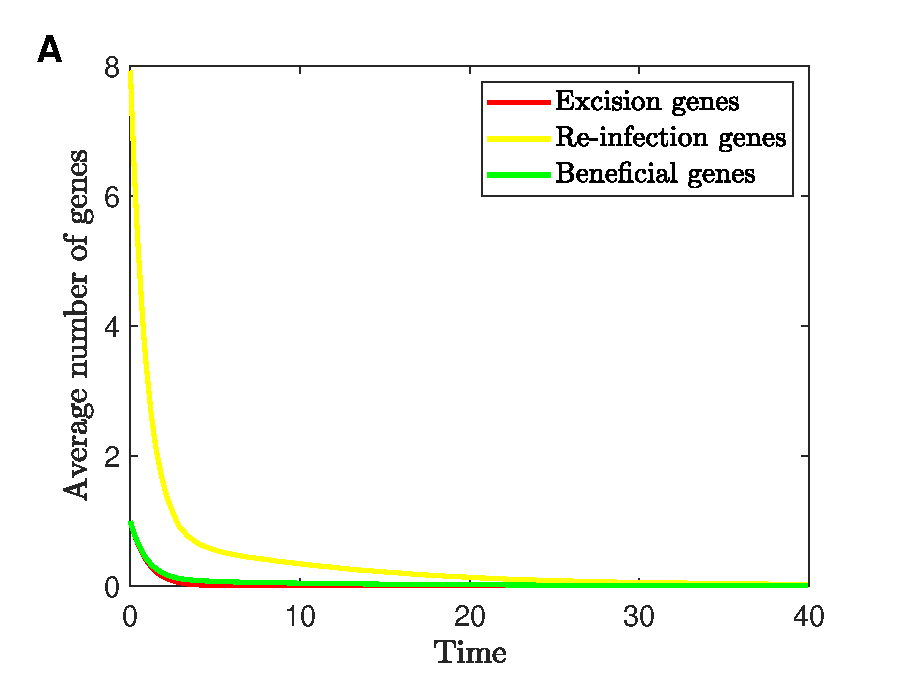
\includegraphics[scale=0.50]{trivSim1}
     \end{subfigure}\hfill
         \begin{subfigure}[t]{0.50\textwidth}
    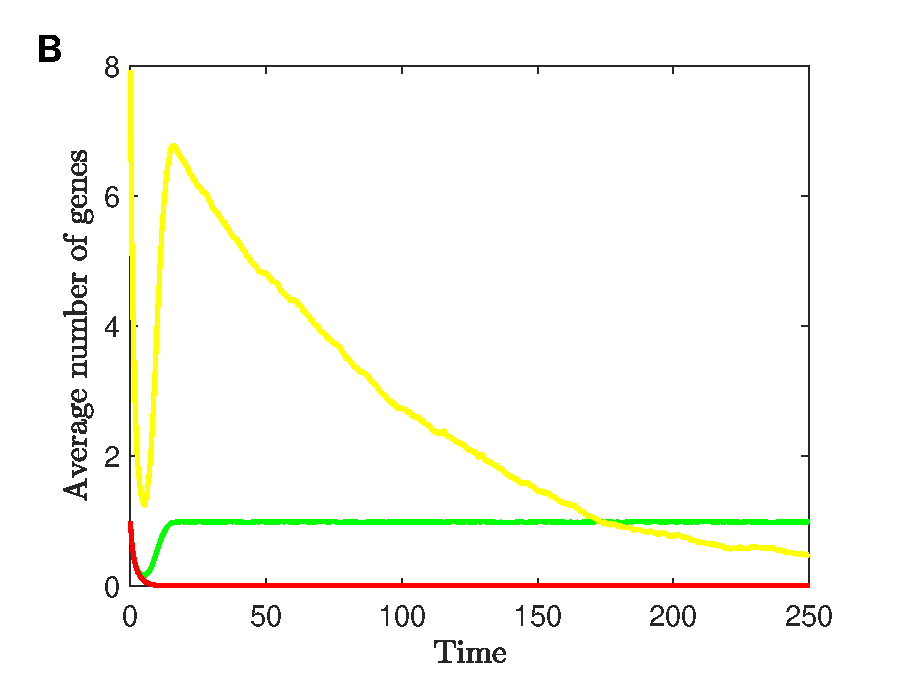
\includegraphics[scale=0.50]{E_bSim1}
    \end{subfigure}\hfill\\  \begin{subfigure}[t]{0.50\textwidth}
        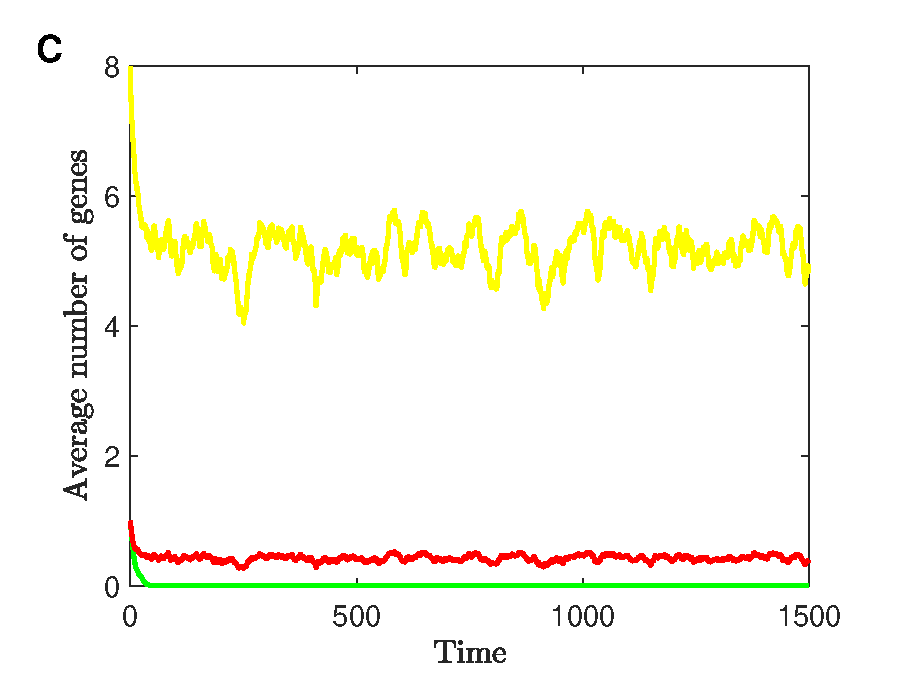
\includegraphics[scale=0.50]{E_liSim}
    \end{subfigure}\hfill   \begin{subfigure}[t]{0.50\textwidth}
    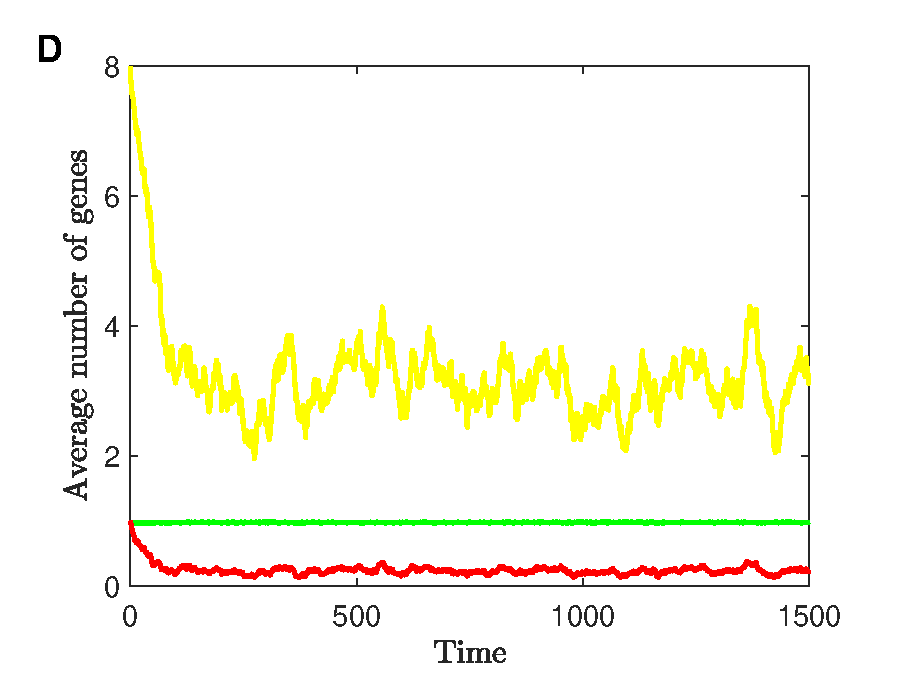
\includegraphics[scale=0.50]{E_libSim}
    \end{subfigure} 
     \caption[Simulations results showing the approach to four possible long-term outcomes.]{Simulations results showing the approach to four possible long-term outcomes:  (A) {\bf Extinction} ($r_S = 0.01 , \, r_D =0.1 , \, r_L =0.2 \, $);  (B) {\bf Domestication} ($r_S = 0.52 , \, r_D =0.01 , \, r_L =0.2  $); (C) {\bf Virulence} ($r_S = 0.02 , \, r_D =0.1 , \, r_L = 2.0  \, $); (D) {\bf Persistence} ($r_S = 1.5, \, r_D =0.05 , \, r_L =1.5  \, $).  In all cases, $r_I=1$, $r_T=0$, $n_B=1$, $n_E=1$ and $n_R=8$. The average number of genes of each type, per prophage, is plotted against time. }
     \label{fig:simresults}
     \end{figure}
 
  We further examined the qualitative features of the prophage population at the persistence equilibrium.  To do this, we  simulated the prophage population with parameter values as described in panel D of Figure \ref{fig:simresults} for 200 generations, and then compared the gene content of prophages of different lengths.  We define all prophages as either ``intact"  or ``incomplete": an intact prophage carries all the genes necessary for excision and re-infection, whereas if any of these genes is missing, the prophage is incomplete. Figure \ref{fig:Biresults}A shows the frequency of each type of gene in intact and incomplete prophages; the percent change in incomplete prophages, as compared to the baseline of an intact prophage, is shown in panel B.  We find that genes involved in excision and re-infection are preferentially lost in incomplete prophages.  
 
 These results are clarified in Figure \ref{fig:Biresults}C, which shows a histogram of prophage lengths (grey bars), along with the gene frequency for each gene type, for prophages of each length.  Thus for example full prophages have 10 genes and have 80\% re-infection genes, 10\% excision genes and 10\% beneficial genes.  We see a bimodal distribution of prophage lengths, with the smallest prophages becoming domesticated, that is, retaining only the gene that benefits the host.
 
  \begin{figure}[H]
    \centering
     \begin{subfigure}[t]{0.30\textwidth} 
    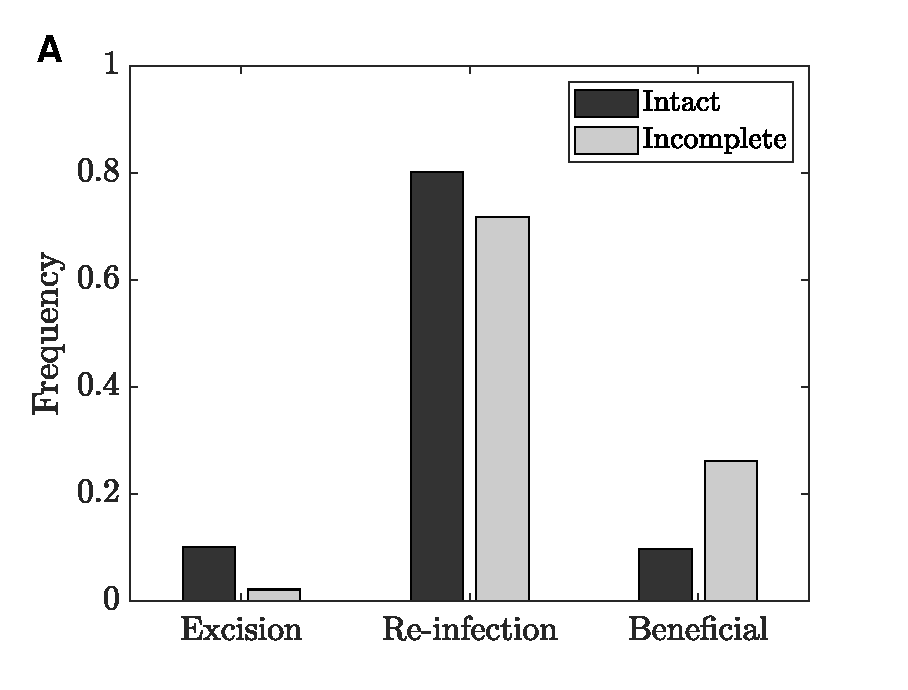
\includegraphics[height=1.8in,width=2.2in]{2Bi1}
     \end{subfigure}\hfill
         \begin{subfigure}[t]{0.30\textwidth}
    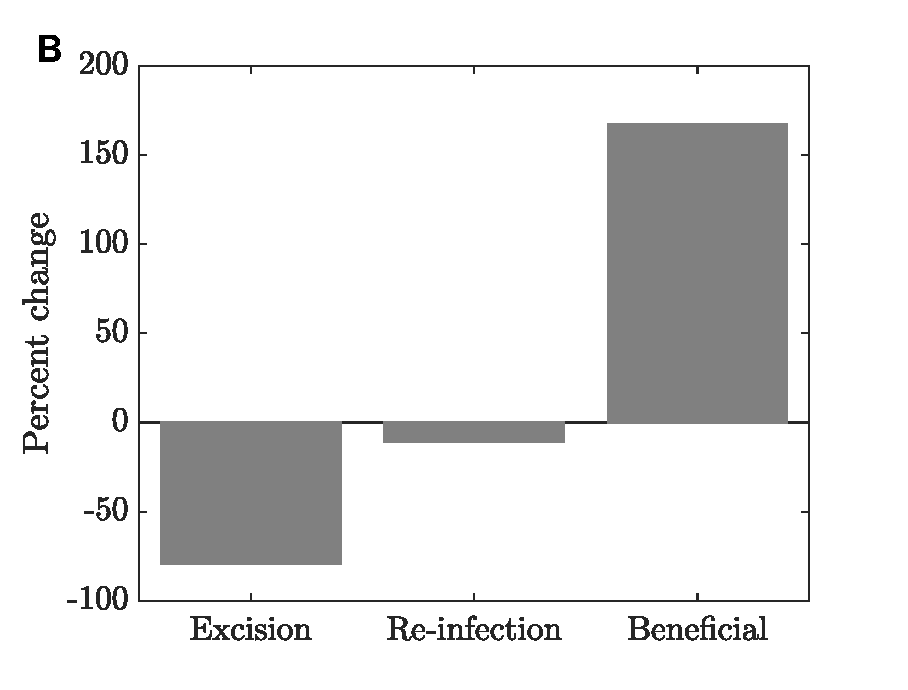
\includegraphics[height=1.8in,width=2.2in]{3Bi1}
    \end{subfigure}\hfill
    \begin{subfigure}[t]{0.30\textwidth}
        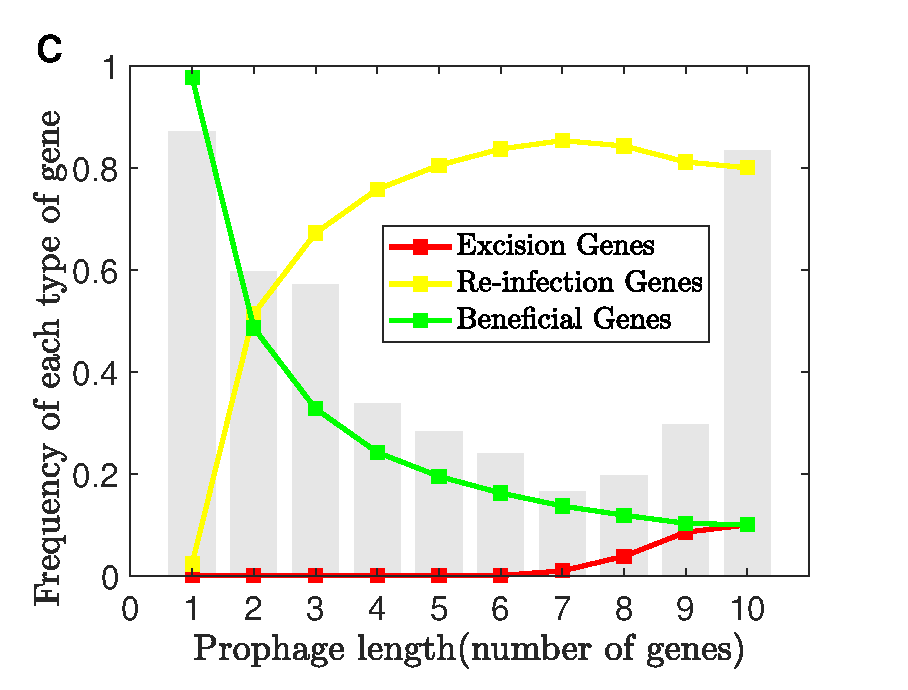
\includegraphics[height=1.8in,width=2.2in]{4Bi1}
    \end{subfigure}\hfill    
     \caption[Gene frequencies in intact and incomplete prophages.]{Gene frequencies in intact and incomplete prophages. (A) Frequency of genes of each type in intact and incomplete prophages, for the computational model simulated at the persistence equilibrium (see text for details); (B) Percent change in gene frequency from intact to incomplete; (C) A histogram of prophage lengths (grey bars), as well as the frequency of gene classes at each length.  We find a bimodal distribution of prophage sizes, with smaller prophages losing the excision and re-infection genes but retaining the beneficial gene.}
     \label{fig:Biresults}
     \end{figure}
     
 
 Fig. \ref{fig:TEsresults} illustrates the effect of adding transposable element disruptions to the computational model. In panel A, despite TE disruptions, the prophage population persists and retains all genes.  Here we have also added a single neutral gene, which has no effect on fitness, for comparison (grey line).  Panel D shows the average number of TE disruptions sustained in each type of gene; TEs accumulate in neutral genes but their presence in functional genes is minimized by purifying selection.  Panels B through F show similar results, except that the rate of TE disruption, $r_T$, and the selective advantage, $r_S$, are altered.  Increasing the transposition rate has the same qualitative effect as increasing the mutation rate, $r_D$, in Table \ref{tab:conditions}; the long-term outcome can change  from persistence (panel A) to either virulence (panel B) or domestication, depending on the value of $r_S$, and then ultimately to extinction (panel C) as $r_T$ increases.
 
 \begin{figure}[H]
    \centering
     \begin{subfigure}[t]{0.30\textwidth} 
    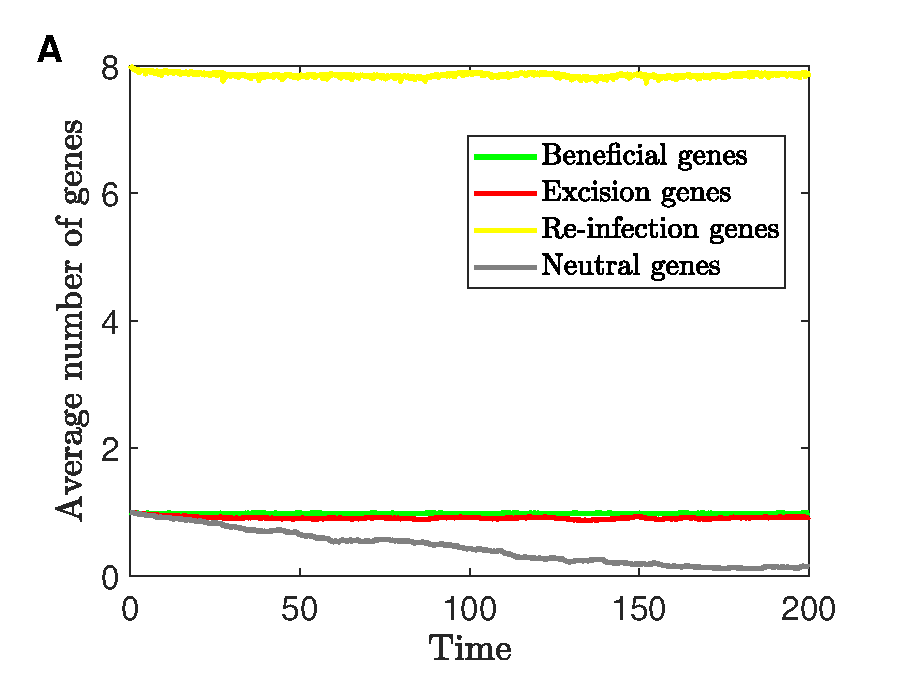
\includegraphics[height=1.8in,width=2.2in]{persisA}
     \end{subfigure}\hfill
         \begin{subfigure}[t]{0.30\textwidth}
    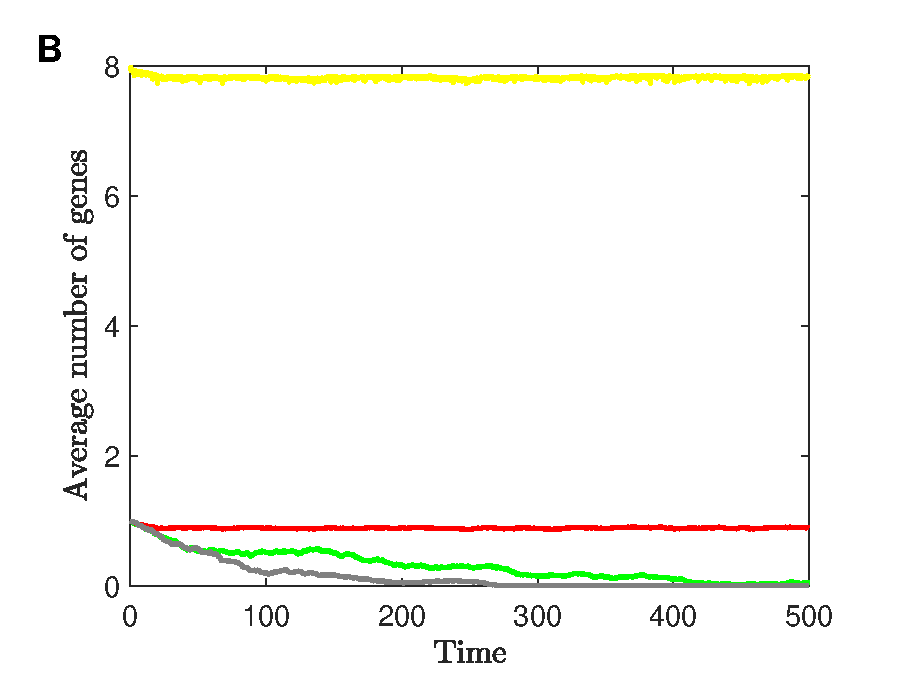
\includegraphics[height=1.8in,width=2.2in]{persisB}
    \end{subfigure}\hfill  
    \begin{subfigure}[t]{0.30\textwidth}
        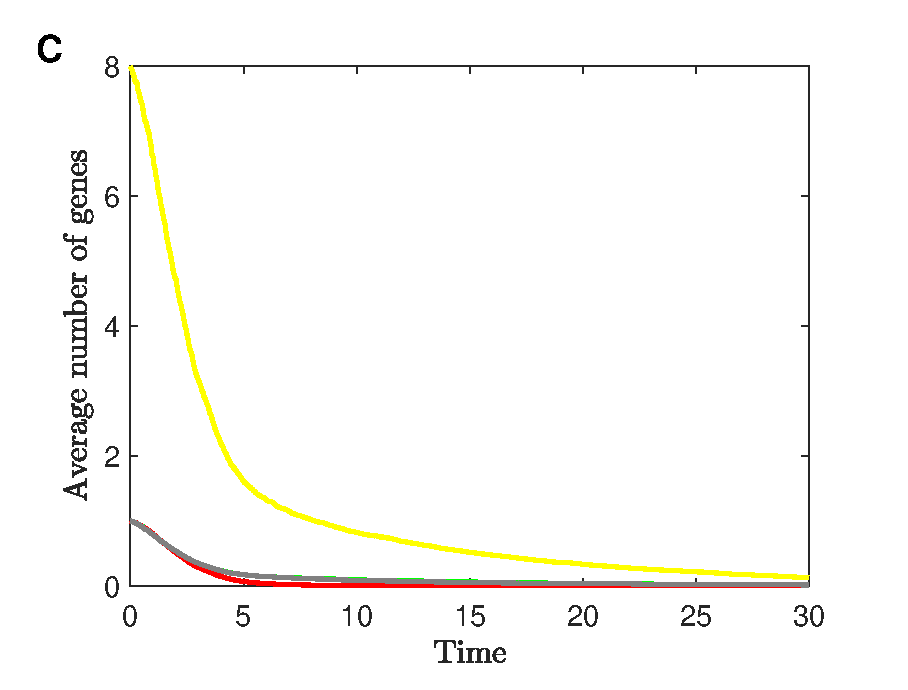
\includegraphics[height=1.8in,width=2.2in]{persisC}
    \end{subfigure}\hfill  \\  
      \begin{subfigure}[t]{0.30\textwidth} 
    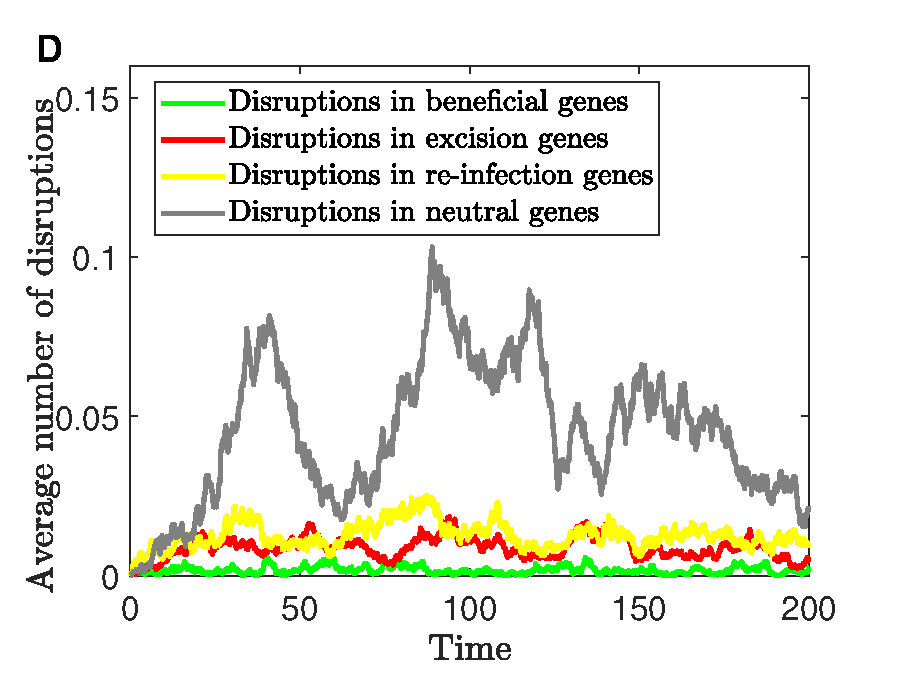
\includegraphics[height=1.8in,width=2.2in]{persisISD}
     \end{subfigure}\hfill
         \begin{subfigure}[t]{0.30\textwidth}
    \includegraphics[height=1.8in,width=2.2in]{persisISE}
    \end{subfigure}\hfill
    \begin{subfigure}[t]{0.30\textwidth}
        \includegraphics[height=1.8in,width=2.25in]{persisISF}
    \end{subfigure}\hfill  
     \caption[The effect of TE disruptions on the long-term outcome for prophage sequences]{The effect of TE disruptions on the long-term outcome for prophage sequences. In panels A through C, the average number of genes of each type per prophage is plotted against time.  As the transposition rate is increased, the long-term prediction for the prophage changes from persistence (panel A) to virulence (panel B) and finally to extinction (panel C).  Panels D through F show the average number of TE disruptions sustained in genes of each type versus time.  TEs accumulate in neutral genes but are limited in functional genes due to purifying selection.  Parameter values are:
     (A and D)  $r_S = 0.52, \, r_T = 0.009$;  (B and E) $r_S = 0.01, \, r_T = 0.01$; (C and F) $r_S = 0.002, \, r_T = 0.1$. In all cases, $r_I=1$, $r_L = 1.2$, $r_D = 0.001$, $n_B=1$, $n_E=1$, $n_R=8$ and $n_N=1$.}
     \label{fig:TEsresults}
     \end{figure}

Again, we simulated the prophage population with parameter values as described in panel D of Figure \ref{fig:simresults} for 5000 generations, but including TE disruptions ($r_T = 0.002$), comparing the gene content of intact and incomplete prophages.  Using the strict definition of ``intact"  or ``incomplete" described above, transposase genes were enriched nearly 400-fold in incomplete prophages (see Supplementary Material).  

This result may be artificially inflated by the fact that only the single beneficial gene can sustain a TE disruption in an intact prophage in our simulations.  In reality, algorithms such as PHASTER are not able to classify prophages as intact based on the certainty that they contain a full complement of functional phage genes.  Instead, approximate metrics are used, based for example on the number of identified phage genes in close proximity in the sequence \cite{arndt_phaster:_2016}. For a better comparison with the data shown in Figure \ref{fig:data4}, we therefore classified prophages as ``intact" if they contained 80\% of more of the possible prophage genes; prophages with less than 80\% were classified as incomplete.

Figure \ref{fig:Biresults80}A shows the frequency of each type of gene in intact and incomplete prophages classified in this way; the percent change in incomplete prophages, as compared to the baseline of an intact prophage, is shown in panel B.  Again we see that genes involved in excision and re-infection are preferentially lost, beneficial genes are preferentially maintained, and transposase genes are substantially enriched in shorter prophages.  

Figure \ref{fig:Biresults80}C shows a histogram of prophage lengths (grey bars), along with the gene frequency for each gene type, for prophages of each length.  A bimodal distribution of prophage lengths is again demonstrated, with the smallest prophages becoming domesticated, that is, retaining only the gene that benefits the host.  We note that transposase genes accumulate in prophages of intermediate length, but are absent from the smallest prophages.

  \begin{figure}[H]
    \centering
     \begin{subfigure}[t]{0.30\textwidth} 
    \includegraphics[height=1.8in,width=2.2in]{BiTe180}
     \end{subfigure}\hfill
         \begin{subfigure}[t]{0.30\textwidth}
    \includegraphics[height=1.8in,width=2.2in]{BiTe280}
    \end{subfigure}\hfill
    \begin{subfigure}[t]{0.30\textwidth}
        \includegraphics[height=1.8in,width=2.2in]{BiTe3o}
    \end{subfigure}\hfill    
     \caption[Gene frequencies in intact and incomplete prophages, when TEs are included.]{Gene frequencies in intact and incomplete prophages, when TEs are included ($r_S = 1.5, \, r_L = 1.5, \, r_D = 0.048, \, r_T = 0.002$). (A) Frequency of genes of each type in intact and incomplete prophages, for the computational model simulated at the persistence equilibrium with TE disruptions (see text for details); (B) Percent change in gene frequency from intact to incomplete; (C) A histogram of prophage lengths (grey bars), as well as the frequency of gene classes at each length.  We find a bimodal distribution of prophage sizes, with TEs accumulating in prophages of intermediate lengths.}
     \label{fig:Biresults80}
     \end{figure} 
 
 \section{Summary and Discussion}
 
 We bring three lines of evidence to bear on the diverse genetic repertoire of active and cryptic prophages.  First, we examine over 50,000 gene annotations from sequenced prophages to demonstrate that genes involved in lytic function -- structural genes such as plate, capsid and portal genes, as well as lysis, lysin and terminase genes -- are preferentially lost in incomplete (presumably cryptic) prophages.  In constrast, three gene classes are enriched: tail fiber, integrase and transposase genes (Fig. 1c, d).
 
 Secondly, a simplified mathematical model predicts that depending on the balance among dynamic processes such as the rates of lysis and infection, selection and mutational degradation, four longterm outcomes are predicted for prophage sequences: the maintenance of an active prophage that also carries host-beneficial genes, the maintenance of an active but virulent prophage, domestication, or extinction (Fig. 3 and Table 3).
 
 Thirdly, a more complex computational approach examines the genetic repertoires of prophages of differing lengths.  The computational model predicts a bimodal distribution of prophage lengths, as observed in a number of recent studies \cite{bobay_pervasive_2014, leplae_aclame:_2010, brueggemann_pneumococcal_2017, crispim_screening_2018}, and consistent with our recent predictions regarding the interplay of selection and mutation on the prophage length distribution \cite{khan_quantifying_2019}.  The computational model also demonstrates that genes involved in excision and re-infection are preferentially lost in shorter prophages (Fig. 5, 7), consistent with the loss of lytic-cycle specific genes observed our bioinformatic analyis (Fig. 1).  This result is intuitively appealing since selection at the level of the host favors loss of intact lytic-cycle alleles, which contribute to greater rates of host lysis and death.  
 
 As summarized above, our bioinformatic analysis supported a previous finding \cite{bobay_pervasive_2014} that some genes are significantly enriched in shorter prophages; in our data these enriched genes included transposases, phage tail protein-encoding genes, and integrases.  Consistent with these data, transposases preferentially accumulated in shorter prophages in our simulation studies, which assumed that transposable elements disrupted gene function and left an identifiable transposase gene sequence as a signature.
 
 Tail fibre genes, in contrast, would be classified as re-infection genes, and thus were not predicted to be enriched in cryptic prophages in our simulations.  Bobay et al. \cite{bobay_pervasive_2014} hypothesize that tail genes may be domesticated by bacterial hosts through the longer-term processes of co-option and evolution of novel function, for example the evolution of bacterial tailocin toxins from phage tail ancestors. For domestication of tail genes in this way, such processes would presumably require a specific combination of multiple accumulated mutations and the appropriate selective environment for a novel function to emerge. These conditions were well beyond the scope of our models here, but modeling the additional complexity of domestication via the accumulation of {\it de novo} adaptive mutations is an interesting idea for future work.
 
The enrichment of integrase genes in short prophages was an interesting and unexpected result of our bioinformatic analysis. Prophages typically possess integrase genes, facilitating chromosomal integration, and excision in conjugation with excisionase \cite{groth_phage_2004, casjens_prophages_2003,  frost_mobile_2005, ptashne_genetic_2004}. %Integrase genes typically mark one end of a prophage and are sufficiently conserved to be recognizable \cite{casjens_prophages_2003}.   
Prophage integrase genes have been used as recognized diagnostic markers for prophages within bacterial genomes \cite{ventura_prophage_2003,tran_sa3mw_2019}, as markers to identify temperate phage genomes \cite{song_prophage_2019}, and as signature genes to measure prophage diversity, and hence, host genome diversity \cite{colavecchio_prophage_2017}.
 %In this study the authors showed that food-associated isolates contain more integrase genes than clinical isolate. 
%1031 temperate phages out of 3540 phage genomes extracted from the NCBI
Based on these facts we were expecting that integrase genes may be missing in incomplete prophages (as suggested for example in \cite{colavecchio_prophage_2017}), yet the opposite trend was observed.

We suggest that integrase genes may be maintained through the evolution of phage-like genetic selfish elements, such as satellite phages and molecular parasites that don’t require the full complement of phage lytic cycle genes but benefit from horizontal transfer among hosts.  Integrase genes are commonly found on mobile genetic elements \cite{domingues_integrons:_2012}; when foreign DNA enters a host cell through horizontal transfer, integrase acts as a catalyst to mediate the process of recombination, thus integrases may facilitate the horizontal transfer of prophage-derived elements. The horizontal transmission of integrase genes along with their neighboring prophage genes would then result in significant enrichment of integrase genes in incomplete prophages.  Although our computational model has not yet incorporated horizontal transmission of full or partial prophages, this hypothesis could be explored more fully in an expanded model that includes horizontal gene transfer. 

 

\addcontentsline{toc}{chapter}{Bibliography}
\bibliographystyle{abbrv}
\bibliography{refrence} 



\chapter{Discussion \& Conclusions}
The study of phage-bacteria interactions involves gigantic numbers \cite{noauthor_microbiology_2011}: if all the viruses on earth were laid end to end they would stretch for 100 million light years; there are $13\times10^{28}$ bacteria in the oceans (100 million times more than the number of stars in the known universe); $1\times10^{31}$ viral infections occur per second in the ocean environment which results in the removal of  20\% to 40\% of the bacterial mass in the oceans per day;  one gram dental plaque contains approximately $1\times10^{11}$ bacteria; a teaspoon of soil  contains $1\times 10^{9}$ microorganisms; bacteria present in the human gut weigh about 1 kg; 8\% of human DNA is of viral origin;  we have only sequenced $1\times10^{-22}$\% of the total DNA on earth.

These quantities, along with the importance of the microorganisms to our ecosystem \cite{gibbons_microbial_2015, graham_microbes_2016}, public health \cite{smith_microbiology_2015}, food, and the possible discovery of new life on distant planets \cite{lopez_inevitable_2019}, have transformed our views about phage-bacteria interaction from being a simple system to a complex and important set of interactions. The intriguing dynamics of phage-bacteria interactions and the urgency of these global issues have invited us to dive deep into this ocean of knowledge. Once immersed in this study, we realized that there are more surprising facts, such as: the amount of temperate phage DNA in bacterial genomes surpasses the amount of DNA in free-living phage \cite{wahl_prophage_2017}; and pathogenic bacteria, responsible for the death and miseries of millions of people,  are domesticating these viral genomes with high frequency \cite{fortier_importance_2013}. In this thesis, we contributed to this vast field. Our contribution is in the form of three projects, called \textbf{Chapter 2}, \textbf{Chapter 3} and \textbf{Chapter 4}, in this investigation. Below we provide details of these projects and the conclusions derived from them. 

Here, we started with a topic directly related to public health, “Phage therapy and antibiotics for biofilm eradication: a predictive model” (\textbf{Chapter 2}). In that chapter, we developed a simple predictive model to capture the effect of the synergistic use of phages and antibiotics in biofilms. For this study, we assumed that bacteria are offering structural resistance (by grouping together, constructing biofilm and developing an EPS structure around the biofilm) to the antibiotic. In this model, we also used the idea of a group defense mechanism, that is, a phage functional response to bacteria resembling a Holling type IV functional response. We were able to show that neither antibiotic nor phages alone can eliminate the biofilm completely, and the synergistic effect of applying phages first and then antibiotics works better. 

Prophages, being the main source of bacterial genome diversity and important factors in bacterial genome evolution, are more abundant in bacterial genomes than previously thought \cite{costa_genomic_2018, mottawea_salmonella_2018}. In \textbf{Chapter 3}, we developed a mathematical model to study the effect of various evolutionary forces acting on prophages. We investigated the model in detail, fitting against some publicly available datasets, and were able to quantify the relative rates of these evolutionary forces in time units expressed in terms of the ``expected prophage lifetime", that is, the average time between lysogeny and induction (see Table \ref{tab:rates}). From these rates, we conclude that:   (1) the time between lysogeny events is about 5 prophage lifetimes, that is, new prophages enter into bacterial genomes at a rate one-fifth of the induction rate; (2) the selection coefficient is 0.5 per prophage lifetime;  (3) on average a prophage has lost only 1\% of its genome at the time of induction; (4) a minimum of two to three prophage genes are required to excise prophage from the bacterial genome.  The relation between prophages and their bacterial hosts is defined to be parasitic or mutualistic depending on the balance between the cost and benefits of the integration of foreign DNA \cite{shapiro_evolution_2018}. The biggest cost due to prophage integration is the possibility of induction, which results in the killing of the bacterial host, although there are other small costs as well, such as energy costs \cite{koonin_evolution_2009}. Our results predict a tipping point between parasitism and mutualism, the point at which cost equals benefit. Our model predicted that the bimodal prophage size distribution is due to the balance between selective advantage (benefit) and induction (cost). The peak on right is due to the lysogeny of new prophages and the peak on left is due to the accumulation of smaller prophages, conferring more benefits to the bacterial hosts than their cost, as shown in Figure \ref{fig:combine}. 

The domestication of defective prophages, the retention of defective prophages that confer some benefit to their hosts, is a common phenomenon in bacterial populations \cite{bobay_pervasive_2014}. We believe that these defective prophages have a prominent role in shaping bacterial genome evolution. The genetic material of domesticated defective prophages may also serve as a tool‐box for other prophages to use for repair through recombination \cite{de_paepe_temperate_2014}. In \textbf{Chapter 4}, ``The genetic repertoire of prophages'' we focus on genes enriched in smaller prophages and the role of evolutionary forces. First, we downloaded data regarding the genetic repertoire for two well-studied prophage databases \cite{bobay_pervasive_2014, leplae_aclame:_2010}, using PHASTER \cite{arndt_phaster:_2016}. The distributions of 53,356 annotated prophage genes identified in 1384 prophage sequences were examined, showing that: (1) genes involved in the lytic life cycle were preferentially lost in smaller prophages; (2) transposes and integrases are significantly enriched in smaller prophages. We also developed an ODE model and computational model to study the effect of these evolutionary forces on the genetic repertoire of prophages.  While the models were able to explain many interesting features of the data, we were unable to explain the enrichment of integrase genes in smaller prophages. 

\section{Future Work}

We believe that the ODE model \ref{modelb}, representing phage-bacteria interaction in bacterial biofilm colonies may have some rich dynamics. We are planning to extend this work further and carry out further detailed bifurcation analysis of the system. In our model, phages and bacteria interact with each other according to the law of mass action and we ignore spatial structure. Several studies have concluded that ignoring the spatial structure of a biological system may lead to inaccuracies \cite{dieckmann_geometry_2000}, and bacterial biofilms have a complex and interesting structure \cite{flemming_biofilms:_2016}. The inclusion of spatial structure in this model is needed to better understand the dynamics of interaction between phages and bacteria in bacterial biofilm colonies.

Prophages are abundant in bacterial genomes and are particularly prominent in pathogenic bacterial genomes \cite{canchaya_impact_2004, brussow_phages_2004}. Prophages from pathogenic bacteria have been shown to encode virulence factors \cite{hyman_bacteriophages_2012}. The insertion of these extra genes in bacterial genomes may increase the bacterial genome size.  But studies have shown that pathogenic bacteria have smaller genomes and fewer genes than their closest non-pathogenic relatives \cite{ moran_microbial_2002, toft_evolutionary_2010}. Gene acquisition and deletion may be the events underlying the emergence and evolution of bacterial pathogens \cite{ochman_genes_2001}. The fact that despite having more prophages in their genomes, pathogen genomes are smaller than the closest non-pathogen relative gives rise to a question: what is the relation between prophages and rates of gene gain and loss, acting on the whole host genome?. The availability of a huge amount of data regarding bacterial pathogens and the usefulness of mathematical modeling can give insights into this question. 

Similarly, mutational deletion is a prominent evolutionary force acting on prophages.  Such mutations make these prophages shorter, eventually resulting in domestication or deletion from the bacterial genome \cite{bobay_pervasive_2014}. Prophages can excise from the bacterial genome randomly or due to some DNA damaging agent, resulting in free life as a temperate phage \cite{nanda_impact_2015}. Does this mutational deletion cause a reduction, over evolutionary time, in the genome size of temperate phages? If not, how can temperate phage keep their genomes intact in the presence of mutational deletions as an important evolutionary force acting on prophages? In other words, what is the role of mutational deletions in the evolution of temperate phages? 

One of the strongest signals obtained from the genetic repertoire data of prophages, in \textbf{Chapter 4}, was the significant enrichment of integrase genes in incomplete prophages (see Table \ref{tab:genes} and Figure~\ref{fig:data}). Full and partial prophage sequences are frequently transferred horizontally through transduction \cite{ fillol-salom_bacteriophages_2019} and related processes such as molecular parasitism by GTAs \cite{lang_gene_2012}. Once foreign DNA enters a host cell through HGT, it needs to recombine with the host genome; integrase acts as a catalyst to mediate the process of recombination, resulting in an increased rate of recombination. Therefore, integrases likely help prophage-derived elements with recombination into the host genome during horizontal transmission. The horizontal transmission of integrase genes along with their neighboring prophage genes may have caused significant enrichment of integrase in incomplete prophages. From this, we hypothesize that in the event of horizontal transmission, a mobile genetic element containing the integrase gene may have a selective advantage over a mobile genetic element lacking the integrase gene. We are planning to explore this hypothesis in much more detail, through an individual-based model like the one developed in Chapter 4, but including more detail such as horizontal gene transfer.

\addcontentsline{toc}{chapter}{Bibliography}
\bibliographystyle{abbrv}
\bibliography{refrence}
%% This adds a line for the Bibliography in the Table of Contents.
%\addcontentsline{toc}{chapter}{Bibliography}
%% ***   Set the bibliography style.   ***
%\bibliographystyle{plain} % (change according to your preference)
%%% ***   Set the bibliography file.   ***
%\bibliography{westernthesis}{}
%\bibliographystyle{elsarticle-harv}
%\bibliography{refrence}
%% ***   NOTE   ***
%% If you don't use bibliography files, comment out the previous line
%% and use \begin{thebibliography}...\end{thebibliography}.  (In that
%% case, you should probably put the bibliography in a separate file
%% and \include or \input it here).

%Appendices.
\begin{appendices}
\chapter{Appendix for Chapter 3}\label{AppA}
\myappendices{Appendix \ref{AppA} }%\byname{AppA}}
\section [Derivation of the PDE model and its steady state solution]{Derivation of the PDE \ref{pde} and its steady state solution }\label{a1}
Let $Q(x,t)$ be the length distribution of prophages of length $x,$ at a time $t.$ Then after time step, $\delta t,$ we have
\begin{eqnarray}\label{d1}
Q(x, t+\delta t) &=& Q(x,t)+ D(x+\delta x)\,P(x+\delta x, t)\, \frac{\delta t}{\delta x}-D(x)\,Q(x,t)\,\frac{\delta t}{\delta x}+ r_{S}S(x)\,Q(x,t)\,\delta t\nonumber\\
&-&r_{I}I(x)\,Q(x,t) \, \delta t+\alpha \, f(x)\, \delta t + \beta \, g(x)\, \delta t. \nonumber
\end{eqnarray}
Using Tylor's series expansion and after simplification we arrive at the following 
\begin{eqnarray}
\frac{Q(x,t+\delta t)- Q(x,t)}{\delta t}& = &   \left(\frac{D(x+\delta x)-D(x)}{\delta x}\right)\,Q(x,t)+D(x+\delta x)\,\frac{\partial Q(x,t)}{\partial x}+ \mathcal{O}(\delta x)\nonumber\\%&+&\mathcal{O}(\delta x)^2+...+r_{S}S(x)\,Q(x,t)-r_{I}I(x)\,Q(x,t)+\alpha \,f(x) \nonumber
\end{eqnarray}
Now taking $\lim_{\delta t\to 0} $ and $\lim_{\delta x\to 0},$ we arrive at
\begin{eqnarray}\label{apppde}
\frac{\partial Q(x,t)}{\partial t} &=& \frac{\partial D(x)}{\partial x}\,Q(x,t)+D(x)\,\frac{\partial Q(x,t)}{\partial x}+r_{S}S(x)\,Q(x,t)-r_{I}I(x)\,Q(x,t)+\alpha \, f(x) + \beta \, g(x)\nonumber\\ 
&=& \frac{\partial }{\partial x}[D(x)\, Q(x,t)]+ [r_{S}S(x)-r_{I}I(x)]\,Q(x,t)+\alpha \, f(x)+ \beta \, g(x).
\end{eqnarray}
If we consider $\lim_{t \to \infty}\,Q(x, t)=P(x)$ and  $D(x) = r_{D}\,x$
then the differential equation generating steady state solution, of the PDE \ref{pde}, is given by \begin{eqnarray}\label{appsol1}
 \frac{d P(x) }{d x}+ \left(\frac{1}{x}+\mathcal{F}(x)\right)\,P(x)+\frac{\alpha}{r_{D}\, x} \, f(x)  + \frac{\beta}{r_{D}\,x} \, g(x) =0
\end{eqnarray}
where $\mathcal{F}(x) = \frac{r_S\, S(x)}{r_D\,x }- \frac{r_{I}\, I(x)}{r_D\, x}.$
Equation (\ref{appsol}) is first order linear ODE and its solution is given by 
\begin{eqnarray}\label{ssol1}
P(x) &=&\frac{-\,e^{-\int{\mathcal{F}}(x)dx} }{r_D\, x}\,\int{(\alpha \,f(x)\, + \, \beta\, g(x))\,e^{\int{\mathcal{F}}(x)dx}dx}+\frac{C}{x}\, e^{-\int{\mathcal{F}}(x)dx},
\end{eqnarray}
where $C$ is a constant of integration.
\section{Results from model selection and data fitting}\label{a2}
The AIC value is the measure of loss of information for the model under consideration and is an ordinal number, used for ranking models. The lowest AIC value corresponds to the best fit.  If the number of data points are small enough compared to the number of parameters then the AIC value is not penalized enough. To remedy this problem a second order Akaike Information criteria, the corrected Akaike Information Criteria (AICc), is defined. The corrected  Akaike Information Criteria (AICc) is given as \citep{burnham_model_2003}:
\begin{eqnarray}\label{aicc}
AIC_c=AIC + \frac{2k(k+1)}{n-(k+1)}.
\end{eqnarray}
As the number of data points becomes large enough, AICc values converge to AIC values and either of these criteria can be used to determine the best fit model amongst the candidate models \citep{burnham_model_2003}. In the tables to follow, we provide both AIC and AICc values, and compute relative probabilities using the AICc values.
  \subsection{Data Set 1}
  \begin{table}[hbt!]
\centering
\begin{tabular}{ p{1cm}p{2cm}p{2cm}p{2cm}p{2cm}p{3cm}  }
\hline
\# & Parameters & AIC & AICc& Log-likelihood & Relative probability (AICc) \\
\hline
1&                        15&          4884.1734&          4884.9642&         -2427.0867&         0.3719\\
2&                        14&          4882.2952&          4882.9860&         -2427.1476&         1\\
3&                        12&          4893.5207&          4894.0322&         -2434.7603&       0.0039\\
4&                        11&          4894.7613&          4895.1920&         -2436.3807&       0.0022\\
5&                         9&          4908.5087&          4908.8014&         -2445.2544&      2.4788e-06\\
6&                         8&          4906.2759&          4906.5097&         -2445.1379&      7.7964e-06\\
7&                         6&          5044.8136&          5044.9499&         -2515.9068&      6.7604e-36\\
8&                         6&          5069.6683&          5069.8042&         -2528.8341&      2.7098e-41\\
9&                         4&          5063.9143&          5063.9788&         -2527.9571&      4.9878e-40\\
\hline
\end{tabular}
\caption[Number of parameters, AIC, AICc values, log-liklihood and the corresponding relative probabilities for Data Set 1.]{Number of parameters, AIC, AICc values, log-liklihood and the corresponding relative probabilities for Data Set 1 \citep{bobay_pervasive_2014}. The best fit model includes a mixed distribution to describe autonomous temperate phages ($g$=3), degradation, induction and selection. The second best fit model is the same model with HGT and has relative probability $0.3791$.}
\label{table:bob}
\end{table}
\newpage
\subsection{Data Set 2}
\begin{table}[hbt!]
\centering
\begin{tabular}{ p{1cm}p{2cm}p{2cm}p{2cm}p{2cm}p{2cm}  }
\hline
\# & Number of Parameters & AIC & AICc& Log-likelihood  & Relative probability \\
\hline
1&                         15&          993.726&          998.583&         -480.863&       0.0016\\
2&                        14&          990.549&          994.797&         -480.275&        0.0108\\
3&                        12&          991.327&          994.492&         -482.663&         0.0126\\
4&                        11&           987.247&          989.937&         -481.624&         0.123\\
5&                         9&          987.197&          989.062&          -483.599&         0.191\\
6&                         8&          984.237&          985.749&         -483.119&          1\\
7&                         6&          1006.929&          1007.855&         -496.464&      1.585e-05\\
8&                         6&          1012.234&          1013.159&         -499.117&       1.117e-06\\
9&                         4&          1004.729&          1005.216&         -497.364&      5.927e-05\\
\hline
\end{tabular}
\caption[Number of parameters, AIC, AICc values and the corresponding relative probabilities for Data Set 2.]{Number of parameters, AIC, AICc values and the corresponding relative probabilities for Data Set 2 \citep{crispim_screening_2018}. The best fit model includes degradation, induction and selection as well as one Gaussian distribution to describe autonomous temperate phages ($g$=1).}
\label{table:desu}
\end{table}
\newpage
\subsection{Data Set 3}
\begin{table}[hbt!]
\centering
\begin{tabular}{ p{1cm}p{2cm}p{2cm}p{2cm}p{2cm}p{2cm}  }
\hline
\# & Number of Parameters & AIC & AICc& Log-likelihood  & Relative probability \\
\hline

 1&                       15&          5671.819&          5672.579&         -2819.909&        0.0318\\
 2&                       14&          5669.819&          5670.489&         -2819.909&        0.0904\\
 3&                       12&          5670.179&          5670.685&         -2822.089&        0.0819\\
 4&                       11&          5667.438&          5667.872&         -2821.719&          0.3347\\
 5&                        9&          5667.461&          5667.766&         -2823.731&         0.3528\\
 6&                        8&          5665.434&          5665.683&         -2823.717&         1\\
 7&                        6&          5731.084&          5731.239&         -2858.542&      5.8167e-15\\
 8&                        6&          5757.726&          5757.880&         -2871.863&      9.5404e-21\\
 9&                        4&          5753.680&          5753.762&         -2871.840&      7.4776e-20\\
\hline
\end{tabular}
\caption[Number of parameters, AIC, AICc values and the corresponding relative probabilities for Data Set 3.]{Number of parameters, AIC, AICc values and the corresponding relative probabilities for Data Set 3 \citep{leplae_aclame:_2010}. The best fit model includes degradation, induction and selection as well as one Gaussian distribution to describe autonomous temperate phages ($g$=1). }
\label{table:aclame}
\end{table}
\addcontentsline{toc}{chapter}{Bibliography}
\bibliographystyle{apa}
\bibliography{refrence}


\chapter{Appendix for Chapter 3}\label{AppB}
\myappendices{Appendix \ref{AppB} }%\byname{AppA}}
\section{Sensitivity Analysis}
\subsection{Sensitivity to the smallest autonomous phage length.}\label{bob30}
We tested fitting model (\ref{pde}) to Data Set 1, but assuming that the smallest autonomous phage to infect \textit{E.~Coli} and \textit{S.~Enterica} has length $\theta$ = 30 kb, as suggested in \cite{bobay_pervasive_2014}. We compared these results to results obtained with $\theta$ = 20 kb, as described in Section 2.2 of the main text. Figure~\ref{fig:comp_PDF} demonstrates that our results are insensitive to the choice of this parameter. 
\begin{figure}[H]
\centering
\includegraphics[scale=0.7]{comp_PDF.eps}
\caption[Results of data fitting are not sensitive to the choice of the parameter $\theta$ representing the genome size of the smallest autonomous temperate phage in kb.]{Results of data fitting are not sensitive to the choice of the parameter $\theta$ representing the genome size of the smallest autonomous temperate phage in kb.  Best fits obtained to Data Set 1 (histogram) for $\theta$ = 20 (blue, solid) and $\theta$ = 30 (red, solid) are indistinguishable.}
\label{fig:comp_PDF}
\end{figure}

\subsection{Rate parameters}

We performed a bootstrap sensitivity analysis for all parameters of the model using Data Set 1.  In brief, we assumed that the best fit model for Data Set 1 represented the true distribution, and resampled this true distribution 335 times, each time creating a simulated data set of 624 observed prophage lengths.  We then subjected each of these data sets to the model fitting exercise described in Section 3 of the main text.  Table \ref{table:sens_p} shows the mean and standard deviations for the relative rate parameters of the model (each rate normalized by the induction rate, $r_I$), after the analysis of 335 simulated data sets.  These results indicate that the quantitative conclusions of our work are relatively insensitive to variations in data sampling; the coefficient of variation (standard deviation/mean) of the degradation rate is largest at 16\%.

\renewcommand{\baselinestretch}{1}
\begin{center}
\begin{table}[H]
\centering
\begin{tabular}{ p{1.6cm}p{5cm}p{2cm}p{2cm}p{2.1cm} }
\hline
Parameter & Description  & Mean & Standard deviation & Coefficient of Variation  \\
\hline 
\\
 $\alpha $   & Relative rate of lysogeny &     0.2078&          0.0118 & 0.0569\\
 $r_D$   & Relative rate of degradation &       0.0125&         0.0021 & 0.1644\\
 $r_S$ &   Relative selection coefficient &    0.5012&     0.0483 & 0.0964\\
% $r_I$ & Relative rate of induction & 1.0000 &  ---& --- \\
% \\
 \hline
\end{tabular}
\caption{Sensitivity analysis of rate parameters. }
\label{table:sens_p}
\end{table}
\end{center}

\renewcommand{\baselinestretch}{1.0}

\subsection [Influx of active phage]{Influx of active phage, $f(x)$}

In addition, this process produced 335 estimates of the influx distribution $f(x)$.  In Figure \ref{fig:sens_f}, we plot the mean of these functions at every value of $x$ (blue line), plus/minus one standard deviation (grey area).  The best fit $f(x)$ from Data Set 1 is also shown for comparison (red line).  These results indicate that the form of $f(x)$ is very tightly constrained by the data, a result that is perhaps not surprising given the large number of data points.

\begin{figure}[H]\centering
\includegraphics[scale=0.7]{f_sens.eps}

\caption[Sensitivity analysis of the prophage influx function.]{Sensitivity analysis of the prophage influx function.  The mean (red) and standard deviation ($\sigma$) of best-fit $f(x)$ curves for all simulated data sets are shown, along with the best-fit $f(x)$ function from the true data (blue).  See text for details.}
\label{fig:sens_f}
\end{figure}
\addcontentsline{toc}{chapter}{Bibliography}
\bibliographystyle{apa}
\bibliography{refrence}
\chapter{Appendix for Chapter 3}\label{AppC}
\myappendices{Appendix \ref{AppC} }%\byname{AppA}}
\section{The influx distribution}
As described in Section 2.2 of the main text, the function $f(x)$ gives the length distribution for prophages that are newly integrating into bacterial genomes.  Here, we note that this is neither the length distribution of active temperate phages, nor is it the length distribution of inducing phage.

To clarify, suppose $A(x)$ is the length distribution of active temperate phages. Let $L(x)$ be the average lysogeny probability for a temperate phage of length $x$.  Since $A(x)$ consists of phages of different classes (lambdoid, mu-like, etc.), we expect that $L(x)$ is not constant in $x$.  In this case, the influx distribution  $f(x)$ is given by
the product $f(x) = A(x)L(x)$.  Thus, unfortunately, we cannot use empirical data describing $A(x)$ to infer $f(x)$.

Similarly, from the model at steady state, the product $P(x)I(x)$ gives the length distribution of excising prophage.  Suppose $R(x)$ gives the probability that a prophage of length $x$ retains the genes required for re-infection (genes involved in replication, packaging, and adsorption, for example).  If re-infection competent phage enter the lysogenic life cycle with probability $L(x)$, we could also express the influx distribution as $f(x) = P(x)I(x)R(x)L(x)$.  Again, we are unable to use $P(x)I(x)$ to directly infer $f(x)$.

Despite these limitations, some qualitative features of $f(x)$ and $A(x)$ appear surprisingly robust.  Along with prophage sequences, the length distribution of 68 dsDNA temperate phages infecting enterobacteria are reported in \cite{bobay_pervasive_2014}.  While the weight of the peaks in this multimodal distribution vary, the number and position of the peaks is strikingly similar with our best fit estimate for $f(x)$ for Data Set 1, as shown in Table \ref{table:sens_f}.

\renewcommand{\baselinestretch}{1}
\begin{table}[hbt!]
\centering
\begin{tabular}{ p{6cm}p{2cm}p{3cm} }
\hline
Feature & Empirical Data & Model Prediction  \\
\hline
\\
 Number of main peaks&     3&          3\\
  Position of first peak&        $\approx 40$ kb&          $\approx38$ kb\\
 Position of second peak &    $\approx 45$ kb &          $\approx 48$ kb\\

 Position of third peak&       $\approx 59$ kb&      $\approx 61$ kb\\
 \\
 \hline
\end{tabular}
\caption[Comparison of the main features of empirical data describing the length distribution of autonomous dsDNA phages.]{Comparison of the main features of empirical data describing the length distribution of autonomous dsDNA phages \citep{bobay_pervasive_2014}, and the best-fit model predictions for the phage influx distribution, $f(x)$. }
\label{table:sens_f}
\end{table}
Similarly, we find that $I(x)P(x)$ yields a surprisingly good approximation for $f(x)$, as illustrated in Figure \ref{fig:IP}, again for Data Set 1.  This suggests that most prophage sequences that retain the genes for necessary for excision also retain the genes necessary for re-infection.

\begin{figure}[t]\centering
\includegraphics[scale=0.7]{IP.eps}
\caption[Comparison of best-fit $f(x)$ with the product $P(x)I(x)$.]{Comparison of best-fit $f(x)$ with the product $P(x)I(x)$; results shown for Data Set 1.}
\label{fig:IP}
\end{figure}
\addcontentsline{toc}{chapter}{Bibliography}
\bibliographystyle{apa}
\bibliography{refrence}
\chapter{Appendix for Chapter 3}\label{AppC1}
\myappendices{Appendix \ref{AppC1} }%\byname{AppA}}
\section{MATLAB code}
In this appendix we are presenting MATLAB \cite{MATLAB:R2018b} code for solving PDE model (\ref{pde}). The MATLAB routine \texttt{fiminsearch} was used to maximize the log-likelihood. The AIC criteria was then used to select the best fit model from all the candidate models.  Here we present code for the full model used to fit the steady state solution of \ref{pde} to Data Set 1 \cite{bobay_pervasive_2014}. This code calculates  selection (\ref{sel}) and induction (\ref{indu}) before fitting the steady state solution to the data. 
The code then maximizes the log-likelihood, which is calculated by the function \texttt{sol\_error}, also provided. 
\begin{lstlisting}
clear all
clc
global pls 
load('prophage_sizes.csv')
pro = prophage_sizes;
pls = pro;
pls=pls/1000; % prophage length in kb
Pinit=  [0.204686704151821   4.099811476589647  15.724017308458798  11.536956361960861  65.822440602842576  27.198192070426217  25.986837564236168   10.382028701765515  41.551463526177145...
         6.882397692568709  0.007780330712747   0.013293852127858   2.799975078907655   0.949368876463170  44.738263580612710   0.020163712415658]; % inatial guess
 options = optimset('MaxFunEvals',2000000);
 Pbest = fminsearch(@sol_error,Pinit);
 Pbest;
 P = Pbest;
\end{lstlisting}
\begin{lstlisting}
function err = sol_error(P)
global pls xs pfinal 
ts = 0:0.01:200;
xs = linspace(0, max(pls), 664);
f= @ (x) abs(P(2))*exp(-(x-(20+abs(P(3)))).^2./abs(P(4)))+ ...
    abs(P(5))*exp(-(x-(20+abs(P(6)))).^2./abs(P(7)))+ ...
    abs(P(8))*exp(-(x-(20+abs(P(9)))).^2./abs(P(10))); % gaussian of incoming phages
g = @(x) abs(P(11))*(-x+max(pls)); % HGT
%%%%%%%%%%%%%%%%%%%%%%%%%%%%%%%%%%%%%%%%%%%%%%
D= @(x) abs(P(12))*x;
dD= @(x) abs(P(12));
%% 
% Calculating induction curve
M1min = 20;  % smallest dsDNA phage
MM= max(pls);
n = abs(P(13)); % minimum number of genes required for induction
M1max = max(pls);
M1 = M1min :0.1: M1max;
b = zeros(length(M1), length(xs));
bsum = zeros (1, length(xs));
i =1;
while i <= length(M1)
L = M1(i);    
m = n+10^-13:0.1: L;
N= 0:0.1:n;
b(i, 1:length(N))=0;
j=1;
while  j<= length(m)       
       b(i, length(N)+j) = ((m(j).^m(j)).*((L-n).^(L-n)))./( (L.^L).*(m(j)-n).^(m(j)-n));  % continuous approximation to probability of induction     
       j= j+1;
end
bsum = bsum + f(L).*b(i, :);
 i = i+1;
end
k=1; 
while k<=length(bsum)
    p =0:0.1:M1min;
    if k > length(p)
    l= k+1 -length(p);
    L= M1(l);
    end    
    L1 = L:0.1:M1max;
    if k<=length(p)
        bsum(k)= bsum(k)./sum(f(M1));
    else
        bsum(k)= bsum(k)./sum(f(L1));
    end
    k=k+1;
end
I = abs(P(14)).*(bsum./max(bsum));
%% 
% Calculating selection curve
%% 
Max = max(pls);
m = 0:0.1:MM;
M1min = floor(abs(P(15)));
M1max = max(cdfx);
M1 = M1min:0.1:M1max;
%Max = 66;
s=  abs(P(15));
s1 = 0:0.1:s;
expec = zeros(1, length(m));
j=length(s1);
i=1;
while j <=length(m)
    M = M1(j-(length(s1)-1)); 
    M2 = M:0.1:M1max;
    if j <= length(s1)
    while i <= length(s1)
    S = (m(i).*s).*((sum(f(M2)./M2))./sum(f(M2)));
    expec(i)=S;
    i = i+1;    
    end
    else
        S = (m(j).*s).*((sum(f(M2)./M2))./sum(f(M2)));
   expec(j)=S;
    end
j = j+1;
end
Sel = abs(P(16)).*expec;
% solving PDE model
deltat = ts(2)-ts(1);
deltax = xs(2)-xs(1);
b = deltat / deltax;
Q=zeros(length(xs), length(ts));
f= abs(P(2))*exp(-(xs-(20+abs(P(3)))).^2./abs(P(4)))+ ...
    abs(P(5))*exp(-(xs-(20+abs(P(6)))).^2./abs(P(7)))+ ...
    abs(P(8))*exp(-(xs-(20+abs(P(9)))).^2./abs(P(10)));
for i = 1:length(xs)    
    if xs(i)<=20
        f(i) = 0;
    end
end
f = f./trapz(xs, f);
D= abs(P(12))*xs;
dD= abs(P(12));
 for k=1:length(ts)-1
  for i=2:length(xs)-1
        
         Q(i,k+1) = Q(i,k)+deltat.*Q(i,k).*dD+b.*D(i)*(Q(i+1,k)-Q(i,k))+ ...
         (Sel(i)-I(i)).*Q(i,k).*deltat+P(1).*(f(i))*deltat+g(xs(i)).*Q(i, k).*deltat;
    
  end     
    Q(:,k+1) = Q(:,k+1)./trapz(xs,Q(:,k+1));
 end
pfinal = cumtrapz(xs,Q(:,length(ts)));
pguess = interp1(xs,Q(:,length(ts)),cdfx);
err = -sum(log(pguess(2:end-1)));
\end{lstlisting}
\addcontentsline{toc}{chapter}{Bibliography}
\bibliographystyle{apa}
\bibliography{refrence}
\chapter{Appendix for Chapter 4}\label{AppD}
\myappendices{Appendix \ref{AppD} }%\byname{AppA}}
\section{Fixed point and stability analysis of system \ref{systemC}}
System \ref{systemC} has six equilibrium points, four of which are biologically meaningful (non-negative).  We will use the notation $E_i  = \left(\bar P_{111}, \bar P_{011}, \bar P_{101}, \bar P_{110}, \bar P_{001}, \bar P_{010}, \bar P_{100}, \bar P_{000}\right)$, where $\bar P_{ber}$ denotes the equilibrium value of $P_{ber}(t)$, and  describe these equilibria below.

1) The fixed point $E_0 = \left(0, 0, 0, 0, 0, 0, 0, 1\right)$ corresponds to the complete elimination of prophages from bacterial genomes. This fixed point always exists. The eigenvalues of the corresponding linearized Jacobian are: $0$,   $-r_D$, $r_S - r_D$, $r_S - 2 r_D$,  $-r_D - r_I$, $r_S - 2 r_D -r_I$, $r_L - 2 r_D - r_I$, and $r_L + r_S - 3 r_D -r_I $. This fixed point is stable if $r_S < r_D$ and $r_L < 2\,r_D + r_I$.

2) The fixed point $E_B = (0, 0, 0, 0, 0, 0, \frac{r_S - r_D}{r_S}, \frac{r_D}{r_S})$, corresponds to the existence of beneficial prophage genes only. This fixed point exists only if $r_S > r_D.$ The eigenvalues of the corresponding Jacobian matrix are: $-r_D$, $-r_S$, $r_D - r_S$, 
$r_D - r_S$, $-r_I - r_S$, $-r_D- r_I$, $r_L - 2 r_D - r_I$, and $r_L - r_D - r_I - r_S $. Thus the conditions for stability are $r_S > r_D$ and $r_L < 2\,r_D + r_I$.

3) The fixed point $E_{LI}$ =  $\left(0, \frac{\alpha\gamma}{r_L\eta}, 0 , 0, \frac{r_D\alpha\gamma}{r_L\eta^2}, \frac{r_D\gamma}{r_L\eta}, 0, \frac{r_D^2\xi}{r_L\eta^2} \right)$, where $\alpha = r_L-r_D$, $\gamma = r_L - 2r_D - r_I$, $\eta = r_L - r_D - r_I$ and $\xi = 2r_L - 2r_D - r_I$. $E_{LI}$ corresponds to the coexistence of lysis and infectious genes, and exists if $r_L > 2r_D + r_I$. Eigenvalues of the corresponding linearized Jacobian are: $r_S-r_D$, $r_S-r_L$, 
$r_D-r_L$, $r_I+r_S-r_L$, $r_I+r_D-r_L$, $r_S+ r_D+r_I-r_L$, $r_I+2\,r_D-r_L$, and $r_I+2\,r_D-r_L$. These eigenvalues are all negative under the two conditions $r_L > 2r_D + r_I$ and $r_S<r_D$.

4) $E_A$ =  
    $\left(\frac{\alpha\beta\gamma}{r_Lr_S\eta}, \frac{r_D\alpha\gamma}{r_Lr_S\eta}, \frac{r_D\alpha\beta\gamma}{r_Lr_S\eta^2},
    \frac{r_D\beta\gamma}{r_Lr_S\eta}
    \frac{r_D^2\alpha\gamma}{r_Lr_S\eta^2}, 
    \frac{r_D^2\gamma}{r_Lr_S\eta},
    \frac{r_D^2\beta\xi}{r_Lr_S\eta^2},
    \frac{r_D^2\beta\gamma}{r_Lr_S\eta^2}, 
    \frac{r_D^3\xi}{r_Lr_S\eta^2}  \right)$,
    where $\beta = r_S - r_D$.
 The eigenvalues of the Jacobian are: $r_D-r_S$,
$r_D-r_L$, $2\,r_D-r_L-r_S$, $r_I+2\,r_D-r_L$, $r_D+r_I-r_L$, 
$r_I+2\,r_D-r_L-r_S$, $r_I+3\,r_D-r_L-r_S$, and $r_I+3\,r_D-r_L-r_S$. These eigenvalues are all negative under the conditions $r_S>r_D$ and $r_L>2r_D + r_I$.
% \addcontentsline{toc}{chapter}{Bibliography}
% \bibliographystyle{apa}
% \bibliography{refrence}
\chapter{Appendix for Chapter 4}\label{AppE}
\myappendices{Appendix \ref{AppE} }%\byname{AppA}}
\section{Transposase enrichment in incomplete prophages.}
As described in the main text, we simulated the prophage population with parameter values $r_S = 1.5, \, r_D =0.048 , \, r_L =1.5,  \, r_T = 0.002$ for 5000 generations to compare the gene content of intact and incomplete prophages.  Using a strict definition for ``intact" prophages, that is, only prophages containing all the genes required for excision and re-infection were considered intact, transposase genes were enriched nearly 400-fold in incomplete prophages (see Figure~\ref{fig:Biresultso}) (A) and (B). When the classification of ``intact'' prophages was relaxed to prophages that contain 90\% or more of the possible prophage genes, the results showed a 5.6-fold increase in transposase genes (see Figure~\ref{fig:Biresultso}) (C) and (D). 
\begin{figure}[H]
    \centering
     \begin{subfigure}[t]{0.50\textwidth} 
    \includegraphics[scale=0.50]{BiTe1o}
     \end{subfigure}\hfill
         \begin{subfigure}[t]{0.50\textwidth}
    \includegraphics[scale=0.50]{BiTe2o.eps}
    \end{subfigure}\hfill\\  \begin{subfigure}[t]{0.50\textwidth}
        \includegraphics[scale=0.50]{BiTe190.eps}
    \end{subfigure}\hfill   \begin{subfigure}[t]{0.50\textwidth}
    \includegraphics[scale=0.50]{BiTe290.eps}
    \end{subfigure} \hfill    
     \caption[Gene frequencies in intact and incomplete prophages, when TEs are included and intact prophagea are defined as sequences containing all the genes required for excision and reinfection.]{Gene frequencies in intact and incomplete prophages, when TEs are included ($r_S = 1.5, \, r_L = 1.5, \, r_D = 0.048, \, r_T = 0.002$). (A) Frequency of genes of each type in intact and incomplete prophages, for the computational model simulated at the persistence equilibrium with TE disruptions; (B) Percent change in gene frequency from intact to incomplete;  for (A) and (B) intact prophagea are defined as sequences containing all the genes required for excision and reinfection; (C) Frequency of genes of each type in intact and incomplete prophages, for the computational model simulated at the persistence equilibrium with TE; (D) Percent change in gene frequency from intact to incomplete; for (C) and (D) intact prophages are defined as sequences containing 90\% or more of the possible prophage genes.}
     \label{fig:Biresultso}
     \end{figure}
% %\addcontentsline{toc}{chapter}{Bibliography}
% \bibliographystyle{apa}
% \bibliography{refrence}
\chapter{Appendix for Chapter 4}\label{AppE1}
\myappendices{Appendix \ref{AppE1} }%\byname{AppA}}
\section{C++ code for computational model.}
Here we present the C++ code, used to carry out all the calculations of the computational model in chapter 4. This code uses the routine "random.h", adopted from \cite{press_numerical_1992}, to generate a random number between 0 and 1.   
\begin{lstlisting}
#include<stdio.h>
#include<math.h>
#include<stdlib.h>
#include<strings.h>
#include"random.h"
#include "getdata.h"

#define MAXNS 31000
#define MAXGENES 40
#define MAXPRINT 2000

long seed=-1;

int main(int argc, char **argv)
{

  float tend;          
  float delt;
  int nsteps;
  int nlys;
  int ninf;
  int nneut;
  int nben;
  int ngenes;
  float rs;
  float rl;
  float rd;
  float ri;
  float rt;
  int Ninit;
  
  short (*prophages)[MAXGENES], (*tmpptr)[MAXGENES];
  short (*newprophages)[MAXGENES];
  short pro1[MAXNS][MAXGENES];
  short pro2[MAXNS][MAXGENES];
  float genemeans[MAXGENES];
  float ismeans[MAXGENES];
  float tempsum[MAXGENES];
  float tempsumt[MAXGENES];
  int occupied[MAXNS];
  int induce[MAXNS];
  int inducible, induciblesum, numben, noinduceflag = 0;
  float ss, css[MAXNS], r, fractiontolose;
  int maxind, i, newi, j, k, ii, jj, lyscapable;
  float ran3(long *);
  void getdata(FILE *,float *, float *,int *, int *, int *, int *, float *, float *, float *, float *, float *, int *);
  int ntoprint, sizeflag=1, sizes[MAXNS], sizehist[MAXGENES+1], ksum=0;

  FILE *fpin, *fpout, *fpout2, *fpout3, *fpout4, *fpout5;

 if (argc>1) seed = -((long)(atof(argv[1])));
 if (argc>2) sizeflag = (int)(atof(argv[2]));

  if ((fpout=fopen("prosim.out","w"))==NULL) {
    fprintf(stderr,"Error opening prosim.out\n");
    printf("\a");
    exit(1);
  }
  if ((fpout2=fopen("genemeans.out","w"))==NULL) {
    fprintf(stderr,"Error opening genemeans.out\n");
    printf("\a");
    exit(1);
  }
  if ((fpin=fopen("prosim.in","r"))==NULL) {
    fprintf(stderr,"Error opening prosim.in\n");
    printf("\a");
    exit(1);
  }
  if (sizeflag)
  if ((fpout3=fopen("sizes.out","w"))==NULL) {
    fprintf(stderr,"Error opening sizes.out\n");
    printf("\a");
    exit(1);
  }
  if ((fpout4=fopen("Ns.out","w"))==NULL) {
    fprintf(stderr,"Error opening Ns.out\n");
    printf("\a");
    exit(1);
  }  
  if ((fpout5=fopen("ismeans.out","w"))==NULL) {
    fprintf(stderr,"Error opening ismeans.out\n");
    printf("\a");
    exit(1);
  }  

  getdata(fpin,&tend,&delt,&nlys,&ninf,&nneut,&nben,&rs,&rl,&rd,... 
  &ri,&rt,&Ninit);
  if (Ninit>=MAXNS) {
    fprintf(stderr,"Error, Ninit too large\n");
    exit(1);
  }  
  nsteps = tend/delt;
  ngenes = nlys+ninf+nneut+nben;
  if (ngenes>=MAXGENES) {
    fprintf(stderr,"Error, too many genes\n");
    exit(1);
  }
  rs = rs*delt;
  rl = rl*delt;
  rd = rd*delt;
  ri = ri*delt;
  rt = rt*delt;
  float big = 0.02;
  if ((rs>big) || (rl>big) || (rd>big) || (rs*nben>big))
    fprintf(stdout,"Error: big changes in one timestep\n");
  prophages = pro1;
  newprophages = pro2;
  ntoprint = (int)((float)nsteps/(float)MAXPRINT);
  if (ntoprint == 0) ntoprint = 1;

  //
  for (int i = 0; i < Ninit; i++) {
    occupied[i] = 1;
    for (int j = 0; j < ngenes; j++) prophages[i][j] = 1;
    }	
  maxind = Ninit;    // maxind is the maximum possible occupied row in prophages		 
//----------TIME LOOP
    for (int istep =0; istep < nsteps; istep++){  
	
//------------------Induction
//
// scan through the prophages, ineducable only if all genes required for induction are present
// also keep track that at least some prophages are ineducable
    induciblesum = 0;
    for (i = 0; i < maxind; i++) {
      inducible = prophages[i][0]; 
      for (j = 1; j < nlys; j++)
	if (prophages[i][j] != -1) inducible = inducible*prophages[i][j];
      if ( (ran3(&seed) < ri) && (inducible >0)) {
	   occupied[i] = 0; 
           for (j=0;j<ngenes;j++) prophages[i][j]=0; }
      induciblesum += inducible;
    }

    if ((noinduceflag ==0) && (induciblesum == 0)) {
      noinduceflag =1 ;
      fprintf(stdout,"There is no more inducible phage in the population at timestep %d of %d.\n",istep,nsteps);
    } 

//knockout the genes that have been degraded
    for (i = 0; i < maxind; i++)
      for (j = 0; j < ngenes; j++)
        if (ran3(&seed) < rd)  prophages [i][j] = 0;

    //if all genes from a given prophage have been knocked out replace the corresponding entry at "occupied" by 0.
    for (i = 0; i < maxind; i++) {
      int sumpro = 0;
      for (j = 0; j < ngenes; j++) sumpro += prophages[i][j];
      if (sumpro == 0) occupied[i] = 0;
    }

//IS insertions change the sequence to -1
    for (i = 0; i < maxind; i++)
      for (j = 0; j < ngenes; j++)
        if (ran3(&seed) < rt)  prophages [i][j] = -1;

   
  j = 0;   // first possible place to put the new prophage
  for (i=0; i<maxind; i++) {
    lyscapable = 1;
    for (k=0; k<nlys+ninf; k++)
      if ((prophages[i][k]==-1)||(prophages[i][k]==0)) lyscapable = 0;
    if (lyscapable==1)  // ran3 is expensive.  don't call unless lyscapable
      if (ran3(&seed) < rl) {   // make a new copy of prophage[i]
        while (occupied[j]==1) j++; //find the next empty spot
        occupied[j] = 1;
        for (k=0; k<ngenes; k++) prophages[j][k] = prophages[i][k]; 
      }
   }   
   if (j>=maxind) maxind = j+1;
   if (j>MAXNS) { fprintf(stderr,"Error: MAXNS exceeded\n"); istep = nsteps;}          

// selection:
// put a copy of each prophage into the next generation with probability rs*(num ben genes)
//  newi will count the number of prophages in the next generation
   newi = -1;
   for (i=0;i<maxind;i++) {
     numben = 0;
     for (j=ngenes-nben;j<ngenes;j++)
       if (prophages[i][j]==1) numben++;
     if (ran3(&seed)<(float)(rs*numben)) {
       newi++;
       for (k=0;k<ngenes;k++) {
         newprophages[newi][k] = prophages[i][k];
       }
       occupied[newi]=1;
       }
   }
/* population size regulation:  Every prophage is copied to the next
   generation with high probability.  If the current population < Ninit,
   every prophage is copied.  If the current population > Ninit, the
   probability is reduced so that on average Ninit are maintained  */

   fractiontolose = 1.0-(float)Ninit/(maxind+newi);
   for (i=0;i<maxind;i++) {
     if (ran3(&seed)>fractiontolose) {
       newi++;
       ksum = 0;
       for (k=0;k<ngenes;k++) {
         newprophages[newi][k] = prophages[i][k];
         ksum += prophages[i][k];
       }
       if (ksum>0) occupied[newi]=1;
     }
   }
   for (i=newi+1;i<maxind+1;i++) occupied[i] = 0;   // after newi, unoccupied
   tmpptr = prophages;
   prophages = newprophages;
   newprophages = tmpptr;
   maxind = newi;   // newi is the population size of the next population


   // be sure to use maxind, not Ninit, now that the popn size is not constant
   if ((float)istep/ntoprint == (int)istep/ntoprint) {
     for (jj = 0; jj < maxind; jj++) sizes[jj] = 0;  //initialize
     for (ii = 0; ii < ngenes; ii++) {
      tempsum[ii] = 0;
      tempsumt[ii] = 0;   // for transposase genes
      sizehist[ii]=0;  // initialize for later
      for (jj = 0; jj <maxind; jj++) {
        if (prophages[jj][ii] == -1) {
	  tempsumt[ii]++;
	  sizes[jj]++;
	}
	else  {
	  tempsum[ii]=tempsum[ii]+ prophages[jj][ii];
	  sizes[jj] += prophages[jj][ii];
	}
      }	
      tempsum[ii] = (float)(tempsum[ii]/((float)maxind));
      tempsumt[ii] = (float)(tempsumt[ii]/((float)maxind));
    }
    sizehist[ngenes]=0;  // last entry in array didn't get initialized yet
    for (jj=0;jj<maxind;jj++)  sizehist[sizes[jj]]++;
    genemeans[0] = 0; genemeans[1] = 0; genemeans[2] = 0 ; genemeans[3] = 0;
    for (i = 0; i < nlys; i++) genemeans[0] = genemeans[0] + tempsum[i];
    for (i = nlys; i < nlys+ninf; i++) genemeans[1] = genemeans[1] + tempsum[i];
    for (i = nlys+ninf; i < nlys+ninf+nneut; i++) genemeans[2] = genemeans[2] + tempsum[i];
    for (i = nlys+ninf+nneut; i < ngenes; i++) genemeans[3] = genemeans[3] + tempsum[i];
    fprintf(fpout2,"%f %f %f %f %f\n",delt*istep,genemeans[0],genemeans[1],genemeans[2], ...
	       genemeans[3]);
    ismeans[0] = 0; ismeans[1] = 0; ismeans[2] = 0 ; ismeans[3] = 0;
    for (i = 0; i < nlys; i++) ismeans[0] = ismeans[0] + tempsumt[i];
    for (i = nlys; i < nlys+ninf; i++) ismeans[1] = ismeans[1] + tempsumt[i];
    for (i = nlys+ninf; i < nlys+ninf+nneut; i++) ismeans[2] = ismeans[2] + tempsumt[i];
    for (i = nlys+ninf+nneut; i < ngenes; i++) ismeans[3] = ismeans[3] + tempsumt[i];
    fprintf(fpout5,"%f %f %f %f %f\n",delt*istep,ismeans[0],ismeans[1],ismeans[2],ismeans[3]);

    if (sizeflag) {
      for (i=0;i<=ngenes;i++) fprintf(fpout3,"%d ",sizehist[i]);
      fprintf(fpout3,"\n");
    }
    fprintf(fpout4,"%d\n",maxind);
   } //end toprint if statement
   if (sizehist[0] == maxind) {
       fprintf(stdout,"Prophage population is extinct\n");
       istep = nsteps;
   }    
  }  //end of loop on istep
  for (i = 0; i < maxind; i++){
      //fprintf(fpout,"%d ",occupied[i]);
      for (j  =0; j < ngenes; j++) fprintf(fpout," %d ",prophages[i][j]);
      fprintf(fpout,"\n");
  }   
  fclose(fpout2);
  fclose(fpout);
  printf("\a");
}  // end of main

\end{lstlisting}
\addcontentsline{toc}{chapter}{Bibliography}
\bibliographystyle{apa}
\bibliography{refrence}
\end{appendices}

%CV only relevant stuff... not full CV.
\addcontentsline{toc}{chapter}{Curriculum Vitae}
%\chapter*{Curriculum Vitae}
\includepdf[pages=-]{cv.pdf}
% \begin{table}[ht]
% \begin{tabular}{ll}
% \textbf{Name:} & \firstname{} \lastname\\
% \textbf{Post-Secondary} & La La School\\
% \textbf{Education and}& La La Land\\
% \textbf{Degrees:}& 1996 - 2000 M.A.\\\\
% & University of Western Ontario\\
% & London, ON\\
% & 2008 - 2012 Ph.D.\\\\
% \textbf{Honours and}& NSERC PGS M\\
% \textbf{Awards:}& 2006-2007\\\\
% \textbf{Related Work}& Teaching Assistant\\
% \textbf{Experience:}& The University of Western Ontario\\
% & 2008 - 2012\\
% \end{tabular}
% \end{table}
% \subsubsection*{Publications:}
% La La
\end{document}

